\documentclass[11pt,a4paper]{report}

\usepackage{a4}
\usepackage{ngerman}
\usepackage{latexsym}
\usepackage[latin1]{inputenc}
\usepackage{pstricks, pst-node, pst-tree}
\usepackage{listings}
\usepackage{graphics}
\usepackage{wrapfig}

\lstset{language=[95]Ada}

\linespread{1.1}

\title{Ada Crypto Lib (ACL) aka libadacrypt-dev\\
  Version 0.1.2 (beta)\\
  Benutzer-Dokumentation }
\author{Christian Forler}
\date{\today}

%Trennung
\hyphenation{dev Gathering Ciphertext Message libacl Byte Word DWord Arrays}
\hyphenation{Crypto Ferguson Initial Hash-funktionen Private}

\begin{document}

\input ngerman.sty
% Gro�-/Kleinschreibung der deutschen Umlaute
\catcode`�=\active \def�{"a}
\catcode`�=\active \def�{"o}
\catcode`�=\active \def�{"u}
\catcode`�=\active \def�{"s}
\catcode`�=\active \def�{"A}
\catcode`�=\active \def�{"O}
\catcode`�=\active \def�{"U}

\maketitle
\tableofcontents

  \chapter{Einleitung}
Bei der  Ada Crypto Library (ACL) handelt es sich um eine freie 
kryptographische Bibliothek f�r Ada. Eines der beiden Hauptziele bei der
Entwicklung dieser Bibliothek war das Design einer
\textbf{selbst sprechenden und sauberen API}. Das andere Hauptziel war es,
einen m�glichst sauberen Programmierstil zu verwenden, der die formale 
Verifikation des Codes erleichtert.
Aus diesem Grund wurde bei der ACL komplett auf folgende ``Features''
verzichtet:
\begin{itemize}
\item access types (Zeiger)
\item inline Assembler
\item tagged types (Objekte)
\item goto statements
\end{itemize}
Auf goto statements und access-types wurde verzichtet, da diese den 
Quelltext un�bersichtlicher machen und Probleme bei der Verifikation des 
Codes auftreten k�nnen. Auf tagged types wurde verzichtet, da hier
Prozeduren und Methoden �berschrieben werden k�nnen, und erst zur Laufzeit 
dynamisch ermittelt wird welche Methode verwendet wird (dynamisches 
dispatching). Hierdurch treten massive Probleme bei Verifikation des
Codes auf. Auf inline Assembler wurde verzichtet, da dies ein sehr unsauberer
Programmierstil ist und dies die starke Typisierung von ADA umgehen kann.
Was nicht gerade den wahren Ada-Weg entspricht.
Durch diese Einschr�nkungen erh�ht sie zwar die Qualit�t des Quelltextes
im Bezug auf Verifizierbarkeit und Sicherheit, f�hrt aber zu einer
schlechteren Performance. 
Wenn Sie also mehr Wert auf Performance als auf ein sauberes Design
legen, dann sollten Sie sich vielleicht nach einer anderen kryptographischen
Bibliothek umsehen. Leider sind mir keine weiteren freie kryptographische
Bibliothek f�r Ada bekannt auf die ich sie jetzt verweisen k�nnte.\\
Dies ACL hat mehr den Status eines \glqq Proof of Concept''.
Es fand weder ein ``Code-Review'' noch ein ``Code-Audit'' statt. 
Bis jetzt ist der Autor der ACL der Einzige,
der sich mit dem Code etwas n�her befasst hat. Es besteht z.B.
durchaus die M�glichkeit, da� sich sicherheitskritisches Material wie der 
Schl�ssel sich nach der Ausf�hrung eines Programms das die ACL verwendet im
RAM ``�berlebt''. Ein Storage-Pool der genau diese Aufgabe �bernimmt ist in 
Planung. Die meisten kryptographische Bibliotheken die auch dieses 
Sicherheitsproblem haben weisen nicht darauf hin. Von solchen Bibliotheken sollte 
man Abstand nehmen, da diese nicht mit offenen Karten spielen.\\
Im folgendem habe ich noch einmal alle  mir bekannten Nachteile der ACL
aufgelistet.  
\begin{itemize}
\item fehlende S�uberung des Stacks und Heaps 
\item kein ``big endian'' Support
\item schlechte Performance
\end{itemize}
In dieser Dokumentation wird kurz auf die Installation und den topologischen 
Aufbau eingegangen. Danach widmet sich diese Dokumentation ausschlie�lich der 
API. Jedes Paket und dessen API wird in einem separaten Kapitel vorgestellt.
Am Ende jedes Kapitels finden Sie ein Anwendungsbeispiel.\\
Falls sie noch Fragen zur ACL haben, einen Fehler finden oder die ACL um
ein bzw. mehrere Pakete erweitern wollen, dann k�nnen  sie
mich per E-Mail unter folgender Adresse kontaktieren: crypto@shortie.inka.de.\\

\subsubsection{TODO-Liste}
\begin{itemize}
\item Optimierung
\item Eigener Storage Pool
\item Erweiterung (Tiger2, RSA-PSS, Poly1305-AES usw.)   
\item Fallunterscheidung f�r die Anwendung des RNG (Windows/Linux)
\end{itemize}

%%%%%%%%%%%%%%%%%%%%%%%%%%%%%%%%%%%%%%%%%%%%%%%%%%%%%%%%%%%%%%%%%%%%%%%%%%%

\section{Installation HOWTO}
\subsection{libadacrpyt-dev}
\subsubsection{Abh�ngigkeiten}
Unter Linux ben�tigen Sie folgende Pakete um die ACL zu installieren:
\begin{itemize}
\item tar 
\item gnat 
\item make
\item bunzip2 
\item binutils
\end{itemize}

\subsubsection{Kompilieren}
Mit der folgenden Befehlssequenzen entpacken und kompilieren sie die ACL sowie 
den beiliegenden Regressionstest.
\begin{itemize}
\item \texttt{tar cjf acl.tar.bz2}
\item \texttt{cd crypto}
\item \texttt{make}
\item \texttt{make acltest}
\end{itemize}

\subsubsection{Testen}
Bevor Sie die ACL installieren sollten Sie unbedingt den Regressionstest
durchf�hren um sicherzustellen, das die ACL auf ihrem System einwandfrei 
arbeitet. Der Regressionstest dauert auf einem PII 450 ungef�hr 30 Sekunden.
Mit dem folgender Befehlssequenz f�hren Sie den Regressiontest aus.\\
\begin{itemize}
\item \texttt{cd test}
\item \texttt{./acltest}
\item \texttt{cd ..}
\end{itemize}

\subsubsection{Installieren}
Wenn bei dem Test kein Fehler auftrat k�nnen sie die ACL mit folgendem
Befehl installieren:\\
\hspace*{1cm} \texttt{su -c ``make install''}\ \\

\subsubsection{Deinstallieren}
Mit dem folgenden Befehl k�nnen sie ACL wieder deinstallieren:\\
\hspace*{1cm} \texttt{su -c ``make uninstall''}\ \\

\subsubsection{Rekompilieren}
Mit der folgenden Befehlssequenzen k�nnen sie ACL neu kompilieren:\\
\begin{itemize}
\item \texttt{make clean}
\item \texttt{make clean-acltest}
\item \texttt{make}
\item \texttt{make acltest}
\end{itemize}

\subsection{libadacrypt}
\subsubsection{Installieren}
Sie k�nnen die ACL auch mit den folgenden Befehlen als shared library 
(libacl.so) installieren:
\begin{itemize}
\item \texttt{make shared}
\item \texttt{make install-shared}
\end{itemize}

\subsubsection{deinstallieren}
Mit dem folgenden Befehl k�nnen sie ACL wieder deinstallieren:\\
\hspace*{1cm} \texttt{su -c ``make uninstall-shared''}\ \\

\subsection{Dokumentation}
Um diese Dokumentation zu erstellen wird das Paket tetex-bin (latex) und
tetex-extra ben�tigt. Wenn n�tig sollte sie diese beiden Pakete installieren.
Mit dem folgenden beiden Befehlen wird die komplette Dokumentation (de+en) 
erstellt und nach \texttt{/usr/local/share/doc/libadacrypt-dev} kopiert.
\begin{itemize}
\item \texttt{make doc}
\item \texttt{su -c ``make install-doc''}
\end{itemize}\ \\
Mit den folgenden beiden Befehlen k�nnen sie die Dokumentationen unter 
 \texttt{/usr/local/share/doc/libadacrypt-dev} deinstallieren und die 
Dokumentation \glqq l�schen''.
\begin{itemize}
\item \texttt{make clean-doc}
\item \texttt{su -c ``make uninstall-doc''}
\end{itemize}


\subsection{Anpassungen}
Im Unterverzeichnis \texttt{src} befindet sich eine Datei \texttt{Makefile}. 
In dieser k�nnen Sie bei den folgende Variablen Anpassungen vornehmen:
\begin{itemize}
\item LIBDIR :  Installationspfad der shared library.
\item INSTDIR : Installationspfad der ACL.
\end{itemize}\ \\
Ausserdem k�nnen sie noch bei den Makefiles in den Unterverzeichnissen von 
\texttt{doc} durch Anpassung der Variablen \texttt{DOCPATH} vornemen.
Diese Variable enth�lt den Installationspfad der entsprechenden Dokumentation.
 

\subsection{Benchmark}
In dem Unterverzeichnis \texttt{bench} befindet sich ein Benchmark, der in einer
sp�teren Version Aussagen �ber die Performance der ACL auf dem eigenen System 
erm�glichen soll. Der Aufbau orientiert sich an dem des Regressionstests. Bisher
wurde eine M�glichkeit zum Messen der Multiplikationsalgorithmen aus dem Package
\texttt{acl.crypto.types.big-numbers} umgesetzt. Der Benchmark generiert dazu
Zufallszahlen, aus denen die Faktoren bestimmt werden. Das Produkt wird durch die
jeweils durch alle implementierten Algorithmen bestimmt und die zur Berechnung
ben�tigte Zeit ausgegeben.\\
Kompilieren und Ausf�hren l�sst sich der Benchmark durch

\begin{itemize}
\item \texttt{cd bench}
\item \texttt{make}
\item \texttt{./aclbench}
\end{itemize}

Durch einen Aufruf des Benchmarks mit Kommandzeilenparameter \texttt{-CSV} lassen
sich die Messungen kommasepariert ausgeben. Dadurch kann man die Ergebnisse 
einfacher in ein Tabellenkalkulationsprogramm importieren und auswerten.\\
Unter Linux:

\begin{itemize}
\item \texttt{./aclbench -CSV > Dateiname.txt}
\end{itemize}

Im Unterverzeichnis \texttt{bench} befindet sich eine Datei \texttt{Makefile}. 
In dieser k�nnen Sie bei den folgende Variablen Anpassungen vornehmen:\\

Kompilieren des Benchmarks ohne Optimierung:
\begin{lstlisting}{}
aclbench.o :
   $(CC) $(CFLAGS) aclbench
   $(BB) $(BFLAGS) aclbench.ali
   $(LL) $(LFLAGS) aclbench.ali
\end{lstlisting}

Kompilieren des Benchmarks mit O3 Optimierung:
\begin{lstlisting}{}
aclbench.o :
   $(CC) $(CFLAGS_O3) aclbench
   $(BB) $(BFLAGS_O3) aclbench.ali
   $(LL) $(LFLAGS_O3) aclbench.ali
\end{lstlisting}

Kompilieren des Benchmarks mit Symbolen f�r \texttt{gdb} oder \texttt{gnatgdb} :
\begin{lstlisting}{}
aclbench.o :
   $(CC) $(CFLAGS_DBUG) aclbench
   $(BB) $(BFLAGS_DBUG) aclbench.ali
   $(LL) $(LFLAGS_DBUG) aclbench.ali
\end{lstlisting}

Kompilieren des Benchmarks mit Symbolen f�r \texttt{gprof} oder \texttt{kprof}:
\begin{lstlisting}{}
aclbench.o :
   $(CC) $(CFLAGS_GPROF) aclbench
   $(BB) $(BFLAGS_GPROF) aclbench.ali
   $(LL) $(LFLAGS_GPROF) aclbench.ali
\end{lstlisting}

Kompilieren des Benchmarks mit Symbolen f�r \texttt{gcov} oder \texttt{ggcov}:
\begin{lstlisting}{}
aclbench.o :
   $(CC) $(CFLAGS_GCOV) aclbench
   $(BB) $(BFLAGS_GCOV) aclbench.ali
   $(LL) $(LFLAGS_GCOV) aclbench.ali
\end{lstlisting}

%%%%%%%%%%%%%%%%%%%%%%%%%%%%%%%%%%%%%%%%%%%%%%%%%%%%%%%%%%%%%%%%%%%%%%%%%%%

\section{Verzeichnis- und Paket-Struktur}
\subsection{Verzeichnis-Struktur}
\begin{itemize}
\item doc : Dokumentation
\item ref : Referenzen und Spezifikationen
\item src : Quellcode 
\item test : Regressionstest
\item bench : Benchmark
\end{itemize}

%%%%%%%%%%%%%%%%%%%%%%%%%%%%%%%%%%%%%%%%%%%%%%%%%%%%%%%%%%%%%%%%%%%%%%%%%%%

\subsection{Paket-Struktur}
Die Ada Crypto Library (ACL) besteht aus den folgenden Paketen (Komponenten).
\begin{description}
\item[Crypto:]\ \\ 
  Dies ist das Wurzelpaket der ACL.
  Alle anderen Pakete der ACL beginnen mit dem 
Pr�fix \textit{Crypto.}
\item[Crypto.Types:] \ \\
  In diesem Paket befinden sich grundlegende Typen der ACL (z.B. Byte)
  und deren  Basisfunktionen.
  Ein Einsatz der ACL ohne Einbindung dieses Paketes ist nur sehr begrenzt 
  m�glich.
\item[Crypto.Types.Big\_Numbers:] \ \\
  Dieses generische Packet unterst�tzt die Arithmetik in $Z_p$ oder 
  $GF(2^m)$. Der Basistyp hierf�hr ist eine modulare n-Bit Zahl.
  Dieses Packet wird f�r die asymetrische Kryptrographie ben�tigt.
\item[Crypto.Types.Elliptic\_Curves:] \ \\
  Dieses generischen Pakete ist das Wurzelpacket f�r elliptische Kurven.
\item[Crypto.Random:] \ \\
  Dieses Paket ist eine Schnittstelle zwischen einem externen
  Pseudozufallsbitgenerator  und der ACL.
\item[Crypto.Symmetric:]\ \\
  Die ist das Wurzelpaket f�r den symmetrische Zweig.
\item[Crypto.Symmetric.Algorithm:]\ \\
  In diesem Zweig des ACL-Baums befinden sich die symmetrische Algorithmen
  f�r symmetrische Blockchiffren und Hashfunktionen.
\item[Crypto.Symmetric.Algorithm.Oneway:]\ \\
  Jeder Algorithmus verf�gt �ber einen Oneway-Algorithmus.
  Symmetrisch Oneway-Algorithmen sind einfach symmetrische Algorithmen die nur 
  in eine Richtung, entweder Ver- oder Entschl�sseln arbeiten.
\item[Crypto.Symmetric.Blockcipher:]\ \\
  Mit Hilfe dieses generische Paketes k�nnen Sie aus einem symmetrischen
  Algorithmus eine Blockchiffre generieren.
\item[Crypto.Symmetric.Oneway\_Blockcipher:]\ \\
  Mit Hilfe dieses generische Paketes k�nnen Sie aus einem symmetrischen
  Oneway-Algorithmus eine Einweg-Blockchiffre generieren.
\item[Crypto.Symmetric.MAC:]
  Dies ist das Wurzelpacket f�r MACs.
\item[Crypto.Symmetric.Mode:]\ \\
  In diesem Zweig befinden sich verschiedene Betriebsmodi f�r Blockchiffren.
\item[Crypto.Symmetric.Mode.Oneway:]\ \\
  In diesem Zweig befinden sich verschiedene Betriebsmodi f�r 
  Einweg-Blockchiffren.
\item[Crypto.Asymmetric:]\ \\
  Dies ist das Wurzelpaket des asymmetrischen Zweigs.
\item[Crypto.Asymmetric.DSA:]\ \\
  Mit Hilfe dieses Pakets k�nnen digitale Unterschriften erstellt und 
  verifiziert werden.
\item[Crypto.Asymmetric.RSA:]\ \\
  Mit Hilfe dieses Paketes lassen sich Daten  asymmetrisch ver- bzw.
  entschl�sseln
\item[Crypto.Hashfunction:]
  Mit Hilfe dieses generische Paketes k�nnen Sie aus einem entsprechenden
  symmetrischen Algorithmus eine Hashfunktion generieren.\\
\end{description}

\begin{figure}
  \scalebox{0.65}{
  \pstree[nodesep=2pt]{\TR{Crypto}}{%
    \pstree{\TR{Types}}{%
      \TR{Big\_Numbers}  \pstree{\TR{Elliptic\_Curves}}{
      \TR{NSS-BF} \TR{SS-BF} \TR{$Z_p$}}}
    \TR{Hashfunction}
    \pstree{\TR{Symmetric}}{%
      \pstree{\TR{Algorithm}}{%
	\Tr{Oneway}}
      \TR{Blockcipher} 
      \TR{MAC}
      \TR{Oneway\_Blockcipher}
      \pstree{\TR{Mode}}{%
	\TR{Oneway}}} % end symmetric
    \TR{Random} 
    \pstree{\TR{Asymmetric}}{%
      \TR{DSA} \TR{RSA} \TR{ECDSA} \TR{ECDH}}
  }
  }
\end{figure}
    

  \chapter{Crypto}

Crypto ist ein leeres Wurzel-Paket. Dieses Paket enth�lt also keinen Code.
Der einzigste Zweck dieses Paketes ist es, einen eindeutigen Namensraum f�r
alle ACL Pakete zu bilden. Da alle Pakete der ACL Kinder dieses Paketes sind,
beginnt der Name jedes Paketes mit dem Pr�fix Crypto (z.B. Crypto.Foo.Bar).


 

  \part{Basics}
\chapter{Crypto.Types}
This package provides the fundamental and derived types with their
basic functionalities for the ACL.

\paragraph{IMPORTANT.} Applying in the ACL by importing the package:
\begin{lstlisting}
  with Crypto.Types;
\end{lstlisting}
%%%%%%%%%%%%%%%%%%%%%%%%%%%%%%%%%%%%%%%%%%%%%%%%%%%%%%%%%%
\section{Elemental Types}
The elemental or primary types here are only for modular types, i.e.,
overflow or underflow of a variable does not cause an exception. If
the result of an operation is not in the value range of the modular
type, then as long as $n:=2**$ Type'Size = Type'Last+1, the value will
be added or subtracted until the result is again in the range.
\begin{lstlisting}{}
  type Bit is mod 2;
  for  Bit'Size use 1;

  type Byte  is mod 2 ** 8;
  for  Byte'Size use 8;

  type DByte  is mod 2 ** 16;
  for  DByte'Size use 16;

  type Word is mod 2 ** 32;
  for  Word'Size use 32;
  type DWord is mod 2 ** 64;
  for  DWord'Size use 64;

  type Mod_Type is mod 2**32;
  for  Mod_Type'Size use 32;
\end{lstlisting}
The type \texttt{Mod\_Type} has the size of a CPU-word, in the ACL it
is 32 bits.

\subsubsection*{Example}
\begin{lstlisting}{Example}
  with Crypto.Types;
  with Ada.Text_IO;
  use Crypto.Types;
  procedure Example_Types is
    A, B : Byte;  -- Byte has a value range from 0 to 255;
  begin
    A := 100;
    B := A + 250; -- Overflow
    A := A - 250; -- Underflow
    Ada.Text_IO.Put_Line("A: " &  A'IMG);
    Ada.Text_IO.Put_Line("B: " &  B'IMG);
  end Example_Types;
\end{lstlisting}
Result of the program:
\begin{lstlisting}{Example}
A:  106
B:  94
\end{lstlisting}

%%%%%%%%%%%%%%%%%%%%%%%%%%%%%%%%%%%%%%%%%%%%%%%%%%%%%%%%
%%%%%%%%%%%%%%%%%%%%%%%%%%%%%%%%%%%%%%%%%%%%%%%%%%%%%%%%

\section{Derived Types}
Derived types are types, which are derived from the elementary
types. Regularly, these are arrays, consisting of elementary
types. \textbf{All non-private arrays consisting of elementary types
  are interpreted as n-bit numbers within the ACL}, where the first
element ('First) is considered to be the most significant and the last
element ('Last) the least significant element of the number. This is a
fundamental characteristic of the ACL.
\subsubsection*{Bit}
\begin{lstlisting}{Bits}
  type Bits is array (Integer range <>) of Bit;
\end{lstlisting}
\subsubsection*{Bytes}
\begin{lstlisting}{Bytes}
  type Bytes is array (Integer range <>) of Byte;
  subtype Byte_Word  is Bytes (0 .. 3);
  subtype Byte_DWord is Bytes (0 .. 7);

  type B_Block32  is Bytes (0 ..  3);
  type B_Block48  is Bytes (0 ..  5);
  type B_Block56  is Bytes (0 ..  6);
  type B_Block64  is Bytes (0 ..  7);
  type B_Block128 is Bytes (0 .. 15);
  type B_Block160 is Bytes (0 .. 19);
  type B_Block192 is Bytes (0 .. 23);
  type B_Block256 is Bytes (0 .. 31);
\end{lstlisting}
The type B\_BlockN consists of a n-bit array, separated into n/8
bytes, e.g., the type \texttt{B\_Block256} is a 256-bit string,
separated into an array of 32 bytes. In Ada, it can be also
represented as a byte array consisting of 32 elements.

\hhline
%%%%%%%%%%%%%%%%%%%%%%%%%%%%%%%%%%%%%%%%%%%%%%%%%%%%%%%%%%%%%%%%%%%%%%%%%%%
\subsubsection*{Words}
\begin{lstlisting}{Words}
  type Words is array (Integer range <>) of Word;
  
  type W_Block128  is Words(0 ..  3);
  type W_Block160  is Words(0 ..  4);
  type W_Block192  is Words(0 ..  5);
  type W_Block256  is Words(0 ..  7);
  type W_Block512  is Words(0 .. 15);
\end{lstlisting}
The type W\_BlockN consists of a n-bit array, separated into n/32
words, e.g., the type \texttt{W\_Block256} is a 256-bit string,
separated into an array of 8 words. In Ada, it can be also represented
as a word array consisting of 8 elements.

\hhline
%%%%%%%%%%%%%%%%%%%%%%%%%%%%%%%%%%%%%%%%%%%%%%%%%%%%%%%%%%%%%%%%%%%%%%%%%%%
\subsubsection*{DWords}
\begin{lstlisting}{DWords}
  type DWords is array (Integer range <>) of DWord;
  
  type DW_Block128   is DWords(0 ..  1);
  type DW_Block256   is DWords(0 ..  3);
  type DW_Block384   is DWords(0 ..  5);
  type DW_Block512   is DWords(0 ..  7);
  type DW_Block1024  is DWords(0 .. 15);
\end{lstlisting}
The type DW\_BlockN consists of a n-bit array, separated into n/64
DWords, e.g., the type \texttt{DW\_Block256} is a 256-bit string,
separated into 4 DWords. In Ada, it can be represented as a DWord
array of 4 elements.

\hhline
%%%%%%%%%%%%%%%%%%%%%%%%%%%%%%%%%%%%%%%%%%%%%%%%%%%%%%%%%%%%%%%%%%%%%%%%%%%

\subsubsection*{Strings}
\begin{lstlisting}{Strings}
  subtype Hex_Byte  is String (1..  2);
  subtype Hex_Word  is String (1..  8);
  subtype Hex_DWord is String (1.. 16);
\end{lstlisting}
The subtype \texttt{Hex\_Byte} is a string, which consists of 2
characters. It can be used to convert a byte to a string in
hexadecimal. The subtype \texttt{Hex\_Word} is used to convert a word
to a string in hexadecimal, and \texttt{Hex\_DWord} is used for a
dword.

\hhline
%%%%%%%%%%%%%%%%%%%%%%%%%%%%%%%%%%%%%%%%%%%%%%%%%%%%%%%%%%%%%%%%%%%%%%%%%%%
\subsubsection*{Message Block Length}
\begin{lstlisting}{Message blocks}
  subtype Message_Block_Length512  is Natural range 0 ..  64;
  subtype Message_Block_Length1024 is Natural range 0 .. 128;
\end{lstlisting}
The two Message\_Block\_Length types indicate the length of the actual
message stored within a message block in bytes. For example, splitting
a 1152-bit message by 512-bit blocks results in three 512-bit
blocks. The actual message length of the last block is 16 ($1152 - 2
\cdot 512 = 128$ bits $= 16$ bytes).  The remaining 384 bits of the
last message block are ''empty'', which means that they do not contain
any part of the original message. These two types are used for message
block padding.  More information about padding can be found in Chapter
\ref{Hash}.

%%%%%%%%%%%%%%%%%%%%%%%%%%%%%%%%%%%%%%%%%%%%%%%%%%%%%%%%%%%%%%%%%%%%%%%%%%%
%%%%%%%%%%%%%%%%%%%%%%%%%%%%%%%%%%%%%%%%%%%%%%%%%%%%%%%%%%%%%%%%%%%%%%%%%%%

\section{Functions and Procedures}
\subsubsection{Bit-Shifting Functions}
\begin{lstlisting}{}
   function Shift_Left  (Value : Natural;
                		    Amount: Natural) return Natural;
   function Shift_Right (Value : Natural;
   						    Amount: Natural) return Natural;
   function Shift_Left  (Value : Byte; Amount : Natural) return Byte;
   function Shift_Right (Value : Byte; Amount : Natural) return Byte;
   function Rotate_Left (Value : Byte; Amount : Natural) return Byte;
   function Rotate_Right(Value : Byte; Amount : Natural) return Byte;
\end{lstlisting}
These functions are intrinsic. They are used to make a transformation
of the value. They can be also applied on values of type
\texttt{DByte, Word, DWord} and \texttt{Mod\_Type}.

The transformations are made on bit positions. For example, calling
the function \texttt{Shift\_Left()} on a value of type \texttt{Word}
with amount 2 causes the value being shifted two bit positions to left
and padded with two zeros at the end.\\
\begin{lstlisting}{}
   function Shift_Block_Left (B_Block: B_Block128; Amount : Natural) return B_Block128;
   function Shift_Block_Right(B_Block: B_Block128; Amount : Natural) return B_Block128;
\end{lstlisting}
The two functions are used to shift a 128-bit block in a bit position
specified by the \texttt{Amount}.

\hhline
%%%%%%%%%%%%%%%%%%%%%%%%%%%%%%%%%%%%%%%%%%%%%%%%%%%%%%%%%%%%%%%%%%%%%%%%%%%
%%%%%%%%%%%%%%%%%%%%%%%%%%%%%%%%%%%%%%%%%%%%%%%%%%%%%%%%%%%%%%%%%%%%%%%%%%%
\subsubsection*{XOR}
\begin{lstlisting}{}
  function "xor" (Left, Right : Bytes)        return Bytes;
  function "xor" (Left: Bytes ; Right : Byte) return Bytes;
  function "xor" (Left, Right : Words)        return Words;
  function "xor" (Left, Right : DWords)       return DWords;
\end{lstlisting}
These functions perform a field-wise concatenation of the two input
fields by using the XOR operation. Left(Left'First) is XORed with
Right(Right'First) till Left(Left'Last) with Right(Right'Last). Note,
in the second function the Right is XORed with Left(Left'Last).\\

\paragraph{Exceptions.} If the lengths of the two values are not
equal, except the second function:\quad\texttt{Constraint\_Bytes\_Error}\,,
\texttt{Constraint\_Words\_Error} or \texttt{Constraint\_DWords\_Error}.

\begin{lstlisting}{}
  function "xor"(Left, Right : B_Block64)    return   B_Block64;
  function "xor"(Left, Right : B_Block128)   return   B_Block128;
  function "xor"(Left, Right : W_Block512)   return   W_Block512;
  function "xor"(Left, Right : DW_Block512)  return   DW_Block512;
  function "xor"(Left, Right : DW_Block1024) return   DW_Block1024;
\end{lstlisting}
The XOR operations on blocks are needed for generic packages to
convert a specific block.

\hhline
%%%%%%%%%%%%%%%%%%%%%%%%%%%%%%%%%%%%%%%%%%%%%%%%%%%%%%%%%%%%%%%%%%%%%%%%%%%
\subsubsection*{AND}
\begin{lstlisting}{}
 function "and"(Left, Right : Bytes) return Bytes;
\end{lstlisting}
The function is applied to make bit-wise AND of two values of equal
length.\\

\paragraph{Exception.} If the lengths of the two values are not
equal:\quad\texttt{Constraint\_Bytes\_Error}.

\hhline
%%%%%%%%%%%%%%%%%%%%%%%%%%%%%%%%%%%%%%%%%%%%%%%%%%%%%%%%%%%%%%%%%%%%%%%%%%%
\subsubsection*{+}
\begin{lstlisting}{}
  function "+" (Left : Bytes;      Right : Byte)   return Bytes;
  function "+" (Left : Byte;       Right : Bytes)  return Bytes;
  function "+" (Left : Words;      Right : Word)   return Words;
  function "+" (Left : Word;       Right : Words)  return Words;
  function "+" (Left : Words;      Right : Byte)   return Words;
  function "+" (Left : DWords;     Right : DWord)  return DWords;
  function "+" (Left : DWord;      Right : DWords) return DWords;
  function "+" (Left : DWords;     Right : Byte)   return DWords;
  function "+" (Left : B_Block128; Right : Byte)   return B_Block128;
\end{lstlisting}
The "+" function adds values in byte positions.  It calculates from
the least significant ('Last) value to the most significant ('First)
value, i.e., from right to left.\\ \textbf{Example:}
\begin{lstlisting}{}
  procedure Example_Add is
 	  A : Byte := 200;
 	  B : Bytes(0..1) := (0 => 100, 1 => 116);
  begin
  	  B := A + B;  -- B   := 2#11001000# + 2#01100100_01110100#
                  -- B(0) = 2#01100100# = 100
                  -- B(1) = 2#00111100# = 60 -- Overflow
  end Example_Add;
\end{lstlisting}

\hhline
%%%%%%%%%%%%%%%%%%%%%%%%%%%%%%%%%%%%%%%%%%%%%%%%%%%%%%%%%%%%%%%%%%%%%%%%%%%
%%%%%%%%%%%%%%%%%%%%%%%%%%%%%%%%%%%%%%%%%%%%%%%%%%%%%%%%%%%%%%%%%%%%%%%%%%
\subsubsection*{ByteN}
\begin{lstlisting}{}
  function Byte0 (W : Word)  return Byte;
  function Byte1 (W : Word)  return Byte;
  function Byte2 (W : Word)  return Byte;
  function Byte3 (W : Word)  return Byte;

  function Byte0 (D : DWord) return Byte;
  function Byte1 (D : DWord) return Byte;
  function Byte2 (D : DWord) return Byte;
  function Byte3 (D : DWord) return Byte;
  function Byte4 (D : DWord) return Byte;
  function Byte5 (D : DWord) return Byte;
  function Byte6 (D : DWord) return Byte;
  function Byte7 (D : DWord) return Byte;
\end{lstlisting}
Let W $\mathtt{: Word  := B0||B1||B2||B3}$,\\
and D $\mathtt{: DWord := B0||B1||B2||B3||B4||B5||B6||B7}$.\\
Then, \texttt{B0} is the most significant byte, and \texttt{B3} of W
and \texttt{B7} of D are the least significant bytes, respectively.
The first function returns B0 of W, the second B1 of W and so on.

\hhline
%%%%%%%%%%%%%%%%%%%%%%%%%%%%%%%%%%%%%%%%%%%%%%%%%%%%%%%%%%%%%%%%%%%%%%%%%%%
\subsubsection*{To\_Bytes}
\begin{lstlisting}{}
  function To_Bytes(X           : Word)   return Byte_Word;
  function To_Bytes(X           : DWord)  return Byte_DWord;
  function To_Bytes(Word_Array  : Words)  return Bytes;
  function To_Bytes(DWord_Array : DWords) return Bytes;
  function To_Bytes(Message     : String) return Bytes;
\end{lstlisting}
These functions convert the input value of different types into a byte
array. The most significant byte of the first element of the input
array becomes the first byte of the returned byte array und the least
significant byte of the last element becomes the last byte of the
returned byte array. For a message in string, it is converted as ASCII
codes stored in a byte array.

\paragraph{Example:}
\begin{lstlisting}{}
  D : DWord      := 16#AA_BB_CC_DD_EE_FF_11_22#;
  B : Byte_DWord := To_Bytes(D);
      -- B(0) := 16#AA#; B(1) := 16#BB#; B(2) := 16#CC#;
      -- B(3) := 16#DD#; B(4) := 16#EE#; B(5) := 16#FF#;
      -- B(6) := 16#11#; B(7) := 16#22#;
\end{lstlisting}
\begin{lstlisting}
  function To_Bytes(B : B_Block64)   return Bytes;
  function To_Bytes(B : B_Block128)  return Bytes;
  function To_Bytes(B : B_Block192)  return Bytes;
  function To_Bytes(B : B_Block256)  return Bytes;
  function To_Bytes(W : W_Block160)  return Bytes;
  function To_Bytes(W : W_Block256)  return Bytes;
  function To_Bytes(W : W_Block512)  return Bytes;
  function To_Bytes(D : DW_Block512) return Bytes;
\end{lstlisting}
These functions convert blocks to bytes in the same principle, they
are needed for generic packages to convert a specific block.

\hhline

%%%%%%%%%%%%%%%%%%%%%%%%%%%%%%%%%%%%%%%%%%%%%%%%%%%%%%%%%%%%%%%%%%%%%%%%%%%
\subsubsection*{R\_To\_Bytes}
\begin{lstlisting}{}
  function R_To_Bytes (X : Word)  return Byte_Word;
  function R_To_Bytes (X : DWord) return Byte_DWord;
\end{lstlisting}
It transforms a Word resp. DWord into a Byte\_Word resp. Byte\_DWord
in reverse order. The most significant byte of X becomes the last
element in the returned byte array and the least significant byte of X
becomes the first element in the returned byte array.

\hhline
%%%%%%%%%%%%%%%%%%%%%%%%%%%%%%%%%%%%%%%%%%%%%%%%%%%%%%%%%%%%%%%%%%%%%%%%%%
\subsubsection*{To\_Word vs. R\_To\_Word}
\begin{lstlisting}{}
  function To_Word (X       : Byte_Word) return Word;
  function To_Word (A,B,C,D : Byte)      return Word;
  function To_Word (A,B,C,D : Character) return Word;

  function R_To_Word (X : Byte_Word)     return Word;
\end{lstlisting}
The first function converts a Byte\_Word into a Word. X'First becomes
the most significant byte of the Word, and X'Last is the least
significant one.  It can transform four bytes (A, B, C, D) to make a
word. Then, A becomes the most significant byte of the word, and D the
least significant byte.  It can also transform four characters (A, B,
C, D) to make a word. The first character (A'Pos) becomes the most
significant byte of the resulted word, and the last character (D'Pos)
the least significant one.

The function \texttt{R\_To\_Word()} makes a word from the Byte\_Word
in reverse order. X'First becomes the least significant byte of the
word, and X'Last becomes the most significant byte of the
word.

\hhline
%%%%%%%%%%%%%%%%%%%%%%%%%%%%%%%%%%%%%%%%%%%%%%%%%%%%%%%%%%%%%%%%%%%%%%%%%%%
\subsubsection*{To\_Words}
\begin{lstlisting}{}
  function To_Words(Byte_Array : Bytes) return Words;
\end{lstlisting}
This function converts a byte array into a word array
(Word\_Array). Byte\_Array'First becomes the most significant byte of
Word\_Array'First and Byte\_Array'Last becomes the least significant
byte of Word\_Array'Last.

\paragraph{Example:}
\begin{lstlisting}{}
  B : Bytes(1..6):= (16#0A#, 16#14#, 16#1E#, 16#28#, 16#32#, 16#3C#);
  W : Words := To_Words(B);
      -- W(D'First) = 16#0A_14_1E_28#
      -- W(D'Last)  = 16#32_3C_00_00# Zero padding
\end{lstlisting}
Input: B $:=\underbrace{B(1)||B(2)||B(3)||B(4)}_{W(0)}
                    \underbrace{B(5)||B(6)}_{W(1)}$\,,\\ \ \\
Output: W $:=W(0)||W(1)$.

\hhline
%%%%%%%%%%%%%%%%%%%%%%%%%%%%%%%%%%%%%%%%%%%%%%%%%%%%%%%%%%%%%%%%%%%%%%%%%%%
\subsubsection*{To\_DWord vs. R\_To\_DWord}
\begin{lstlisting}{}
  function To_DWord   (X : Byte_DWord) return DWord;
  function R_To_DWord (X : Byte_DWord) return DWord;
\end{lstlisting}
The function \texttt{To\_DWord()} transforms a value of Byte\_DWord
into a DWord.  X'First becomes the most significant byte of the
resulted DWord, X'Last becomes the least significant byte.  While the
function \texttt{R\_To\_DWord()} transforms a Byte\_DWord into a DWord
in reverse order. X'First becomes the least significant byte of the
resulted DWord, and X'Last becomes the most significant byte.

\hhline
%%%%%%%%%%%%%%%%%%%%%%%%%%%%%%%%%%%%%%%%%%%%%%%%%%%%%%%%%%%%%%%%%%%%%%%%%%%
\subsubsection*{To\_DWords}
\begin{lstlisting}{}
  function To_DWords (Byte_Array : Bytes) return DWords;
\end{lstlisting}
It transforms a byte array into a DWord array
(DWord\_Array). Byte\_Array'First becomes the most significant byte of
the DWord\_Array'First, and Byte\_Array'Last becomes the least
significant byte of DWord\_Array'Last.

\paragraph{Example:}
\begin{lstlisting}{}
  B : Bytes(1..10) := (16#0A#, 16#14#, 16#1E#, 16#28#, 16#32#,
                       16#3C#, 16#46#, 16#50#, 16#5A#, 16#64#);
  D : DWords := To_DWords(B);
      -- D(D'First) = 16#0A_14_1E_28_32_3C_46_50#
      -- D(D'Last)  = 16#5A_64_00_00_00_00_00_00#
\end{lstlisting}
\hhline
%%%%%%%%%%%%%%%%%%%%%%%%%%%%%%%%%%%%%%%%%%%%%%%%%%%%%%%%%%%%%%%%%%%%%%%%%%%
\subsubsection*{To\_String}
\begin{lstlisting}{}
  function To_String(ASCII : Bytes) return String;
\end{lstlisting}
It transforms a byte array to a string. Thereby every element of the
byte array will be interpreted as an ASCII-Code.

\hhline
%%%%%%%%%%%%%%%%%%%%%%%%%%%%%%%%%%%%%%%%%%%%%%%%%%%%%%%%%%%%%%%%%%%%%%%%%%%
\subsubsection*{To\_Hex}
\begin{lstlisting}{}
  function To_Hex(B : Byte)  return Hex_Byte;
  function To_Hex(W : Word)  return Hex_Word;
  function To_Hex(D : DWord) return Hex_DWord;
\end{lstlisting}
These functions transform values of Byte, Word or DWord to strings,
which display in hex form.

\paragraph{Example:}
\begin{lstlisting}{}
  B : Word  := 0;
  W : DWord := 16#AA_BB_CC_DD_EE_FF#;
  HB:Hex_Word :=To_Hex(B);  -- HB="00_00_00_00"
  HW:Hex_DWord:=To_Hex(W);  -- HW="00_00_AA_BB_CC_DD_EE_FF"
\end{lstlisting}

\hhline
%%%%%%%%%%%%%%%%%%%%%%%%%%%%%%%%%%%%%%%%%%%%%%%%%%%%%%%%%%%%%%%%%%%%%%%%%%%
\subsubsection*{To\_Block}
\begin{lstlisting}{}
  function To_B_Block64 (B : Bytes) return B_Block64;
  function To_B_Block128(B : Bytes) return B_Block128;
  function To_B_Block192(B : Bytes) return B_Block192;
  function To_B_Block256(B : Bytes) return B_Block256;
\end{lstlisting}
These functions transform bytes to certain block types.

\hhline
%%%%%%%%%%%%%%%%%%%%%%%%%%%%%%%%%%%%%%%%%%%%%%%%%%%%%%%%%%%%%%%%%%%%%%%%%%%
\subsubsection{Is\_Zero}
\begin{lstlisting}{}
  function Is_Zero(Byte_Array  : Bytes)  return Boolean;
  function Is_Zero(Word_Array  : Words)  return Boolean;
  function Is_Zero(DWord_Array : DWords) return Boolean;
\end{lstlisting}
These functions return ''True'' if all fields of the array parameter
contain value ''0'', otherwise, ''False'' is returned.

\hhline
%%%%%%%%%%%%%%%%%%%%%%%%%%%%%%%%%%%%%%%%%%%%%%%%%%%%%%%%%%%%%%%%%%%%%%%%%%%
%%%%%%%%%%%%%%%%%%%%%%%%%%%%%%%%%%%%%%%%%%%%%%%%%%%%%%%%%%%%%%%%%%%%%%%%%%%
\subsubsection{Padding}
\begin{lstlisting}{}
   procedure Padding(Data           : in  out Bytes;
                     Message_Length : in      Word;
                     Data2          : out     Bytes);
   procedure Padding(Data           : in  out Words;
                     Message_Length : in      Word;
                     Data2          : out     Words);
   procedure Padding(Data           : in  out DWords;
                     Message_Length : in      Word;
                     Data2          : out     DWords);
\end{lstlisting}
The padding procedures fill the data with zero bytes/words/dwords,
together with a counter of the padded zero bytes/words/dwor
ds. \texttt{Data} is the message to be padded, and the term
\texttt{Message\_Length} specifies the actual length of the
message. The message corresponds to the following range of
\texttt{Data}: \texttt{Data(Data'First)..Data(Data'First+Message\_Length-1)}. \\
\texttt{Data2} is used in special situations, normally \texttt{Is\_Zero(Data2)} = True.

\paragraph{Exceptions:}
\texttt{Message\_Length} is greater than the length of
\texttt{Data}:\quad\texttt{Constraint\_Message\_Length\-\_Error}.\\ If
the lengths of \texttt{Data} and \texttt{Data2} are not
equal:\quad\texttt{Constraint\_Length\_Error}.\\ \ \\ 
\texttt{Data2} is used in the following two situations:
\begin{itemize}
\item Message\_Length = Data'Length:\quad no zero bytes/words/dwords
  will be padded to \texttt{Data}, and Data2'Last := Data'Length-1\,;
\item Message\_Length+1 = Data'Length:\quad only one zero
  byte/word/dword is padded, and there is no more space for the
  counter. To solve the problem, Data2 is initialized with zero
  bytes/words/dwords, and Data2'Last := Data'Length.
\end{itemize}
\textbf{Example:}
\begin{lstlisting}{}
  procedure Example_Padding is
    X: Bytes(1..9) := (1=>2, 2=>4, 3=>6, 4=>8, 5=>9, others=>1);
    Y: Bytes(1..9);
  begin
    Padding(X,5,Y);
    for I in X'Range loop
        Put(X(I)'Img);
    end loop;
    New_Line;
    for I in Y'Range loop
        Put(Y(I)'Img);
    end loop;
  end Example_Padding;
\end{lstlisting}
\begin{itemize}
\item N = 5\\
\qquad X: 2 4 6 8 9 0 0 0 3
\item N = 8\\
\qquad X: 2 4 6 8 9 1 1 1 0\\
\qquad Y: 0 0 0 0 0 0 0 0 9
\item N = 9\\
\qquad X: 2 4 6 8 9 1 1 1 1\\
\qquad Y: 0 0 0 0 0 0 0 0 8
\end{itemize}

  \chapter{Crypto.Random}
\section{Einf�hrung}
Dieses Paket greift defaultm��ig auf ``dev/random/'' zu.
Unter Linux ist \\``/dev/random'' ein Pseudodevice das kryptographisch sichere
Pseudozufallsbits liefert. Wenn sie ein Betriebsystem verwenden das kein 
solches Pseudodevice besitzt, dann k�nnen sie dies mit Hilfe von mit 
Brian Warners ``Entropy Gathering Daemon''(EGD), der unter
\textit{http://www.lothar.com/tech/crypto/} zu finden 
ist,  nachinstallieren. Der EGD ist ein Userspace-Implementierung des 
Linux-Kernel-Devices ``dev/random/'', das kryptograpisch sichere
Zuallsbits generiert.\\
Im privaten Teil befindet sich die Variable ``Path''. Diese Variable gibt den
Pfad zu einer Datei, Named Pipe oder Ger�t das krytograpisch sichere
Zufallsbits enth�lt an.  Dadurch sind Sie in der Lage die ACL auch an eine
kryptograpisch sichere (Pseudo-)Zufallsbitquelle eines nicht POSIX kompatiblen
Betriebsystems wie Windows XP anbinden.\\
Weiterhin besteht die M�glichkeit unter Windows den Marsaglia- RNG zu benutzen.
Er ist ein lagged- Fibonacci Sequenz Generator und erzeugt 24-Bit real numbers
im Intervall [0,1].\\
Eigenschaften: Kombination zweier unterschiedlicher Generatoren, welche fort-
laufende Bits erzeugen. Diese werden durch zwei weitere Generatoren zu einer 
Tabelle Kombiniert.
Die Prozedur ''Start'' initialisiert diese Tabelle, welche von der Funktion 
''Next'' genutzt wird um die n�chste Zufallszahl zu generieren.

\section{API}
\subsection{Prozeduren}
\begin{tabular}{p{\textwidth}}
  \begin{lstlisting}{}
    procedure Read(B : out Byte);
    procedure Read(W : out Word);
    procedure Read(D : out DWord);
  \end{lstlisting}
  Bei diesen drei Prozeduren wird B, W oder D mit Bits aus der
  verwendeten Pseudozufallsbit-Quelle gef�llt.\\ \ \\
  \hline\\
\end{tabular}

\begin{tabular}{p{\textwidth}}
  \begin{lstlisting}{}
    procedure Read(Byte_Array  : out Bytes);
    procedure Read(Word_Array  : out Words);
    procedure Read(DWord_Array : out DWords);
  \end{lstlisting}\\
  Diese drei Prozeduren wirden die �bergebenen Arrays mit Bits aus der 
  verwendeten Pseudozufallsbit-Quelle gef�llt. \\ \ \\
\end{tabular}

\begin{tabular}{p{\textwidth}}
  \begin{lstlisting}{}
    procedure Start(
    New_I : Seed_Range_1 := Default_I;
    New_J : Seed_Range_1 := Default_J;
    New_K : Seed_Range_1 := Default_K;
    New_L : Seed_Range_2 := Default_L);
  \end{lstlisting}\\
  \\ \ \\
\end{tabular}

\subsection{Exceptions}
\begin{tabular}{p{\textwidth}}
  \begin{lstlisting}{}
    Random_Source_Does_Not_Exist_Error : exception;
  \end{lstlisting}\\
  Diese Ausnahme wird aufgerufen, wenn kein (kryptograpisch sicherer) 
  Pseudozufallsbit-Quelle gefunden wurde.\\ \ \\
  \hline\\
  \begin{lstlisting}{}
    Random_Source_Read_Error : exception;
  \end{lstlisting}\\
  Wenn ein Lesefehler bei einem Zugriff auf die Pseudozufallsbit-Quelle 
  auftritt, wird die folgende Aufnahme ausgeworfen. \\ \ \\
  \hline\\
\end{tabular}

\begin{lstlisting}{}
\end{lstlisting}

  \chapter{Crypto.Symmetric}
\section{Funktion}
Dies ist das Wurzelpaket f�r die symmetrische Kryptographie.
Dieses Paket erm�glicht dem symmetrischen Teil den direkten Zugriff auf 
\texttt{Crypto.Types}  und \texttt{Crypto.Random}. Diesen beiden Pakete
stellen grundlegende Typen und  Basisfunktionen f�r den symmetrischen Teil der
ACL zur Verf�gung.\\
 Das Herzst�ck der symmetrischen Krypographie bilden in der 
ACL Blockchiffren. In dem folgenden Abschnitt wird der Aufbau einer solchen
innerhalb der ACL erl�utert.
 
\section{Blockchiffren}
\subsubsection{Logischer Aufbau}
Eine Blockchiffre ist ein drei logische Schichten unterteilt. Wobei man
als Anwendungsprogrammierer nur die API der h�chsten Schicht verwenden sollte. 
Denn nur mit dieser API ist eine sicher Nutzung einer Blockchiffre garantiert.

\subsubsection{1. Schicht: Algorithmus}
Auf dieser Ebene befindet sich der nackte Algorithmus einer symmetrischen 
Chiffre. Die API der einzelnen Algorithmen ist identisch und dient als 
Schnittstelle f�r die Blockchiffen-Schicht.
Bei jedem  Algorithmus wird die Quelle auf der er beruht genannt.
Damit ist es m�glich sich mit Hilfe der Quelle von der Korrektheit der 
Implementierung zu �berzeugen. 
Es ist auf keinen Fall eine schlechte Idee dies auch zu tun. Mehrere 
Informationen zu den einzelnen Algorithmen und Chiffren erfahren Sie im 
n�chsten Kapitel.\\ \ \\
\textbf{Bemerkung:}\\
Verwenden sie die API dieser Schicht nur um eine Blockchiffre zu 
generieren. Verwenden Sie sie auf keinen Fall f�r einen anderen Zweck.
Es gibt kein Szenario in dem dies einen Sinn ergibt. 
Diese API dient wirklich nur als Schnittstelle f�r die 2. Schicht.


\subsubsection{2. Schicht: Blockchiffre}
Auf dieser Ebene wird aus einem Algorithmus eine Blockchiffre im unsicheren
ECB-Modus (Electronic Code Book) generiert.
Verwenden sie diese API nur, wenn Sie sich auch mit symmetrischen 
Blockchiffren auskennen.
Diese API dient eigentlich nur als Schnittstelle f�r die 3. Schicht.
In Kapitel \ref{block} wird beschrieben wie man aus einem Algorithmus 
eine Blockchiffre generiert.


\subsubsection{3. Schicht: Modus}
Diese Schicht versetzt eine Blockchiffre in einen vern�nftigen Modus. Es gibt 
verschiedene Modi f�r verschiedene Szenarien die alle ihre Vor- und Nachteile 
haben. Alle unterst�tzen Modi und deren Vor- und Nachteil werden in dem
Kapitel \ref{modus} ausf�hrlich beschrieben.

\begin{figure}
  \begin{center}
    \huge
    \begin{tabular}{|c @{\ } c|}\hline
      III. & Modus\\
      \hline
      II. & Blockchiffre\\
      \hline
      I. & Algorithmus\\
    \hline
    \end{tabular}
  \end{center}
\caption{Die 3-Schichten-Architektur einer symmetrischen (Block-)chiffre}
\end{figure}

\subsubsection{Bemerkung}
Mit dieser 3. Schichten Architektur ist es auch m�glich Strom-Chiffren zu
implementieren. Man muss dazu aus er 1. Ebene eine Prozedur zur Verf�gung
stellen die die n�chsten n-Bit des Keystreams liefert. Damit kann man
eine Oneway-Blockchiffre (Kapitel \ref{oneblock}) konstruieren und diese in
den Oneway-OFB oder den Oneway-Counter-Modus versetzen. 
Im Moment beinhaltet die ACL  noch keinen Strom-Chiffre.
Es ist aber geplant die Strom-Chiffre Helix \cite{helix} zu implementieren.


  \chapter{Crypto.Symmetric.Algorithm}\label{Algorithm}
All child packages of the package \texttt{Crypto.Symmetric.Algorithm}
are symmetric ciphers or hash functions. They have direct access to
individual operations, which use a cipher or a hash function. However
users should use the existing API.

%%%%%%%%%%%%%%%%%%%%%%%%%%%%%%%%%%%%%%%%%%%%%%%%%%%%%%%%%%%%%%%%%%%%%%
%%%%%%%%%%%%%%%%%%%%%%%%%%%%%%%%%%%%%%%%%%%%%%%%%%%%%%%%%%%%%%%%%%%%%%

\section{Symmetric Ciphers}
\subsubsection*{General}
The following procedures are defined and used within symmetric ciphers
of the ACL.
\begin{itemize}
\item One procedure \texttt{Prepare\_Key()}; it generates a cipher key
  from the delivered value.\\ \textbf{Example:}
\begin{lstlisting}{}
  procedure Prepare_Key(Key       : in  B_Block128;
                        Cipherkey : out Cipherkey_Type);
\end{lstlisting}
\item One procedure \texttt{Encrypt()}; it converts the input
  plaintext into a output ciphertext.\\

\noindent\textbf{Example:}
\begin{lstlisting}{}
  procedure Encrypt(Cipherkey  : in  Cipherkey_Type;
                    Plaintext  : in  B_Block128;
                    Ciphertext : out B_Block128);
\end{lstlisting}
\item One procedure \texttt{Decrypt()}; it recovers the input
 ciphertext to associated plaintext.\\

\noindent\textbf{Example:}
\begin{lstlisting}{}
  procedure Decrypt(Cipherkey  : in  Cipherkey_Type;
                    Ciphertext : in  B_Block128;
                    Plaintext  : out B_Block128);
\end{lstlisting}
\end{itemize}

%%%%%%%%%%%%%%%%%%%%%%%%%%%%%%%%%%%%%%%%%%%%%%%%%%%%%%%%%%%%%%%%%%%
%%%%%%%%%%%%%%%%%%%%%%%%%%%%%%%%%%%%%%%%%%%%%%%%%%%%%%%%%%%%%%%%%%%

\subsection{AES}\label{AES}
Advanced Encryption Standard (AES) is one of the best-known ciphers
which was officially standardized by the U.S. National Institute of
Standards and Technology (NIST) in 2001 \cite{AES-FIPS}.  Originally
it was called Rijndael, the name was a combination of the names of the
two inventors, Joan Daemen and Vincent Rijmen. The AES algorithm has a
fixed block size of 128 bits and a key size of 128, 192, or 256 bits.
During the AES algorithm, the input plaintext will be transformed
through a round transformation function 10, 12 or 14 times depending
on its key length, and the final output is the ciphertext
\cite{AES-FIPS}. The number of cycles of repetition are as follows:
\begin{itemize}
\item 10 rounds of repetition for 128 bit keys.
\item 12 rounds of repetition for 192 bit keys.
\item 14 rounds of repetition for 256 bit keys.
\end{itemize}
\subsubsection*{API of AES with 128 bit keys:}
\begin{lstlisting}{}
  type Cipherkey_AES128 is private;
  procedure Prepare_key128(Key       : in  B_Block128;
                           Cipherkey : out Cipherkey_AES128);
  procedure Encrypt128(Cipherkey  : in  Cipherkey_AES128;
                       Plaintext  : in  B_Block128;
                       Ciphertext : out B_Block128);
  procedure Decrypt128(Cipherkey  : in  Cipherkey_AES128;
                       Ciphertext : in  B_Block128;
                       Plaintext  : out B_Block128);
\end{lstlisting}
\subsubsection*{API of AES with 192 bit keys:}
\begin{lstlisting}{}
  type Cipherkey_AES192 is private;
  procedure Prepare_key192(Key       : in  B_Block192;
                           Cipherkey : out Cipherkey_AES192);
  procedure Encrypt192(Cipherkey  : in  Cipherkey_AES192;
                       Plaintext  : in  B_Block128;
                       Ciphertext : out B_Block128);
  procedure Decrypt192(Cipherkey  : in  Cipherkey_AES192;
                       Ciphertext : in  B_Block128;
                       Plaintext  : out B_Block128);
\end{lstlisting}

\subsubsection*{API of AES with 256 bit keys:}
\begin{lstlisting}{}
  type Cipherkey_AES256 is private;
  procedure Prepare_key256(Key       : in  B_Block256;
                           Cipherkey : out Cipherkey_AES256);
  procedure Encrypt256(Cipherkey  : in  Cipherkey_AES256;
                       Plaintext  : in  B_Block128;
                       Ciphertext : out B_Block128);
  procedure Decrypt256(Cipherkey  : in  Cipherkey_AES256;
                       Ciphertext : in  B_Block128;
                       Plaintext  : out B_Block128);
\end{lstlisting}

%%%%%%%%%%%%%%%%%%%%%%%%%%%%%%%%%%%%%%%%%%%%%%%%%%%%%%%%%%%%%%%%%%
%%%%%%%%%%%%%%%%%%%%%%%%%%%%%%%%%%%%%%%%%%%%%%%%%%%%%%%%%%%%%%%%%%

\subsection{Blowfish}
Blowfish was designed in 1993 by Bruce Schneier. It uses a key of
variable length (here the length 128-bit is used) and a 64-bit block
cipher. Blowfish has a key-expansion part and a part of 16-round
Feistel network for data encryption \cite{DBLP:conf/fse/Schneier93}.
\subsubsection*{API of Blowfish:}
\begin{lstlisting}{}
  type Cipherkey_Blowfish128 is private;
  subtype B_Block is Bytes;
  procedure Prepare_Key128(Key      :in  B_Block128;
                          Cipherkey :out Cipherkey_Blowfish128);
  procedure Encrypt128 (Cipherkey  : in  Cipherkey_Blowfish128;
                        Plaintext  : in  B_Block64;
                        Ciphertext : out B_Block64);
  procedure Decrypt128 (Cipherkey  : in  Cipherkey_Blowfish128;
                        Ciphertext : in  B_Block64;
                        Plaintext  : out B_Block64);
\end{lstlisting}

%%%%%%%%%%%%%%%%%%%%%%%%%%%%%%%%%%%%%%%%%%%%%%%%%%%%%%%%%%%%%%%%%%
%%%%%%%%%%%%%%%%%%%%%%%%%%%%%%%%%%%%%%%%%%%%%%%%%%%%%%%%%%%%%%%%%%

\subsection{Serpent}
Serpent is designed for 128-bit block ciphers, and was one of the five
finalists in the Advanced Encryption Standard (AES) contest. If you
put a high value on security and not such a high value on performance,
then you can try this block cipher. The implementation is based on the
Ada-Reference-Implementation by Markus G. Kuhn. Temporarily there is
only API for 256-bit cipher key. API for 128-bit and 192-bit keys is
in planning.
\subsubsection*{API of Serpent:}
\begin{lstlisting}{}
  type Cipherkey_Serpent256 is private;
  procedure Prepare_Key256(Key       : in  B_Block256;
                           Cipherkey : out Cipherkey_Serpent256);
  procedure Encrypt256(Cipherkey  : in  Cipherkey_Serpent256;
                       Plaintext  : in  B_Block128;
                       Ciphertext : out B_Block128);
  procedure Decrypt256(Cipherkey  : in  Cipherkey_Serpent256;
                       Ciphertext : in  B_Block128;
                       Plaintext  : out B_Block128);
\end{lstlisting}

%%%%%%%%%%%%%%%%%%%%%%%%%%%%%%%%%%%%%%%%%%%%%%%%%%%%%%%%%%%%%%%%%%
%%%%%%%%%%%%%%%%%%%%%%%%%%%%%%%%%%%%%%%%%%%%%%%%%%%%%%%%%%%%%%%%%%
\subsection{Triple DES(3DES, TDES, TDEA)}
Triple DES is the common name for the Triple Data Encryption Algorithm
(TDEA or Triple DEA), which applies the Data Encryption Standard (DES)
algorithm to each data block three times, and a TDES key is made of
three DES keys \cite{DES-FIPS}. The 192-bit key is decomposed before
encryption in three 64-bit keys. Due to that DES is software-relative
slow, TDES is the slowest block cipher. It is assumed that this cipher
can not be broken, because DES is over 20 years studied by the best
cryptoanalysts on its weakness. The idea comes from the book
\texttt{Applied Cryptography} by Burce
Scheier\footnote{http://www.schneier.com/book-applied.html, Dec
  2012.}.
\subsubsection*{API of Triple DES:}
\begin{lstlisting}{}
  type Cipherkey_TDES is private;
  procedure Prepare_Key(Key       : in  B_Block192;
                        Cipherkey : out Cipherkey_TDES);
  procedure Encrypt(Cipherkey  : in  Cipherkey_TDES;
                    Plaintext  : in  B_Block64;
                    Ciphertext : out B_Block64);
  procedure Decrypt(Cipherkey  : in  Cipherkey_TDES;
                    Ciphertext : in  B_Block64;
                    Plaintext  : out B_Block64);
\end{lstlisting}
\newpage
%%%%%%%%%%%%%%%%%%%%%%%%%%%%%%%%%%%%%%%%%%%%%%%%%%%%%%%%%%%%%%%%%
%%%%%%%%%%%%%%%%%%%%%%%%%%%%%%%%%%%%%%%%%%%%%%%%%%%%%%%%%%%%%%%%%
\subsection{Twofish}
Twofish is one of the five finalists of the Advanced Encryption
Standard contest, with a block size of 128 bits and a key of length up
to 256 bits. It uses the 16-round Feistel network with a bijective F
function, a transform, a bitwise rotation and a key schedule
\cite{Twofish}. The implementation is based on the C-Reference
implementation by Niels Ferguson and the twofish
specification\footnote{http://www.schneier.com/twofish.html}. In the
ACL it is implemented with 128, 192 or 256 bit keys.
\subsubsection*{API of Twofish with 128 bit keys:}
\begin{lstlisting}{}
  type Cipherkey_Twofish is private;
  subtype Cipherkey_Twofish128 is Cipherkey_Twofish;
  procedure Prepare_Key128(Key      : in  B_Block128;
                           Cipherkey: out Cipherkey_Twofish128);
  procedure Encrypt128(Cipherkey    : in  Cipherkey_Twofish128;
                       Plaintext    : in  B_Block128;
                       Ciphertext   : out B_Block128);
  procedure Decrypt128(Cipherkey    : in  Cipherkey_Twofish128;
                       Ciphertext   : in  B_Block128;
                       Plaintext    : out B_Block128);
\end{lstlisting}
\subsubsection*{API of Twofish with 192 bit keys:}
\begin{lstlisting}{}
  subtype Cipherkey_Twofish192 is Cipherkey_Twofish;
  procedure Prepare_Key192(Key      : in  B_Block192;
                          Cipherkey : out Cipherkey_Twofish192);
  procedure Encrypt192(Cipherkey    : in  Cipherkey_Twofish192;
                       Plaintext    : in  B_Block128;
                       Ciphertext   : out B_Block128);
  procedure Decrypt192(Cipherkey    : in  Cipherkey_Twofish192;
                       Ciphertext   : in  B_Block128;
                       Plaintext    : out B_Block128);
\end{lstlisting}
\subsubsection*{API of Twofish with 256 bit keys:}
\begin{lstlisting}{}
  subtype Cipherkey_Twofish256 is Cipherkey_Twofish;
  procedure Prepare_Key256(Key      : in  B_Block256;
                           Cipherkey: out Cipherkey_Twofish256);
  procedure Encrypt256(Cipherkey    : in  Cipherkey_Twofish256;
                       Plaintext    : in  B_Block128;
                       Ciphertext   : out B_Block128);
  procedure Decrypt256(Cipherkey    : in  Cipherkey_Twofish256;
                       Ciphertext   : in  B_Block128;
                       Plaintext    : out B_Block128);
\end{lstlisting}

%%%%%%%%%%%%%%%%%%%%%%%%%%%%%%%%%%%%%%%%%%%%%%%%%%%%%%%%%%%%%%%%%
%%%%%%%%%%%%%%%%%%%%%%%%%%%%%%%%%%%%%%%%%%%%%%%%%%%%%%%%%%%%%%%%%

\section{Hash Functions}\label{AlgorithmHash}
The iterative hash functions in the ACL can be called through a
Low-Level-API or High-Level-API.
\subsubsection*{Excursion: Iterative Hash Functions}
An iterative hash function $H$ decomposes a message $M$ into $r$
message blocks $m_i$ ($1\leq i \leq r$) of length $n$. All message
blocks will be hashed sequentially. To generate a hash value $h$ for
the complete message $M$, the intermediate outputs are also inputs for
the next round.  In general there exists: $h_i:= H(m_i,h_{i-1})$. For
$i=1$, $h_1:=H(M_1,h_0)$ will be applied, hereby $h_0$ is an initial
value, and will be initialized at the beginning. Messages whose length
is not multiple of $n$ will be inflated by a function
\texttt{Padding()} before encryption until the length is multiple of
$n$.

\subsubsection*{High-Level-API}
The High-Level-API is made of 3 procedures, which calculate hash value
of messages in string, bytes or file names in
string.\\

\noindent\textbf{Example:}
\begin{lstlisting}{}
  procedure Hash  (Message  : in String; Hash_Value: out W_Block160);
  procedure Hash  (Message  : in Bytes;  Hash_Value: out W_Block160);
  procedure F_Hash(Filename : in String; Hash_Value: out W_Block160);
\end{lstlisting}

\subsubsection*{Low-Level-API}
The Low-Level-API of a hash function has:
\begin{itemize}
\item One procedure \texttt{Init()}; it initializes the hash context (\texttt{This}).\\
\textbf{Example:}
\begin{lstlisting}{}
	procedure Init(This 		: in out Hash_Interface);
\end{lstlisting}
\item One procedure \texttt{Round()}; a message block (not the last block) will be hashed.\\
\textbf{Example:}
\begin{lstlisting}{}
	procedure Round(This 					: in out 	Hash_Interface;
                  Message_Block : in 		  W_Block512);
\end{lstlisting}
\item One function \texttt{Final\_Round()}; the last message block
  (\texttt{Last\_Message\_Block}) will be inflated and the final hash
  value is returned. Because of the \texttt{Padding()} function, the
  length of the last message block in byte (Last\_Message\_Length)
  should be passed as a parameter.\\

\noindent\textbf{Example:}
\begin{lstlisting}{}
 function Final_Round(This 		    : in out Hash_Interface;
										Last_Message_Block  : W_Block512;
										Last_Message_Length : Message_Block_Length512)
										return W_Block160;
\end{lstlisting}
\end{itemize}

\subsection{SHA-1}\label{SHA-1}
SHA-1 is a cryptographic hash function for 160-bit message blocks. SHA
stands for "Secure Hash Algorithm". SHA-1 was one of the most widely
used hash functions. In 2005, security flaws were identified in SHA-1
by X. Wang, Y.L. Yin und H.Yu, namely that a mathematical weakness
might exist \cite{DBLP:conf/crypto/WangYY05a}. Due to this new
discovery, it is now not advisable to use this hash function. The only
reason why the ACL supports this kind of hash function is its
tremendous degree of process in standard protocols such as digital
signature standard. But this hash function is expected to be no more
supported by the ACL, so you'd better use other hash functions if
possible. \\ \textbf{Remark:}\\ The performance of SHA-1 is slower
than SHA-256.
\subsubsection*{API}
\begin{lstlisting}{}
  -- high level API
  procedure Hash(Message : in String ; Hash_Value : out W_Block160);
  procedure Hash(Message : in Bytes  ; Hash_Value : out W_Block160);
  procedure F_Hash(Filename: in String; Hash_Value : out W_Block160);
  -- low level API
	procedure Init(This 		: in out SHA1_Interface);
	procedure Round(This 	: in out 	SHA1_Interface;
								 Message_Block: in 		W_Block512);
	function Final_Round(This 		    : in out SHA1_Interface;
											Last_Message_Block  : W_Block512;
											Last_Message_Length : Message_Block_Length512)
											return W_Block160;
\end{lstlisting}
\textbf{Exceptions:}
\begin{itemize}
\item If the message length is greater than $2^{64}-1024$:\quad
  \texttt{SHA1\_Constraint\_Error}.
\item In the procedure \texttt{F\_Hash()}, if the file can not be
  opened:\quad\texttt{File\_Open\_Error}.
 \item In the procedure \texttt{F\_Hash()}, if the size of the read
   data is smaller than 0:\quad\texttt{File\_Read\_Error}.
\end{itemize}

%%%%%%%%%%%%%%%%%%%%%%%%%%%%%%%%%%%%%%%%%%%%%%%%%%%%%%%%%%%%%
\subsection{SHA-256}
SHA-256 is a cryptographic hash function with a 256-bit output (hash
value), and it is a member of SHA-2 family, which is based on
SHA-1. This hash family has a hash value in sufficient length and
makes significant changes in security compared to the SHA-1 hash
function. Since this hash family works with 8*32-bit words, its use in
32-bit processors worths a consideration. If possible, SHA-1 should be
replaced by this new generation of SHA-2 hash family.
\subsubsection*{API}
\begin{lstlisting}{}
  -- high level API
  procedure Hash(Message : in Bytes ; Hash_Value : out W_Block256);
  procedure Hash(Message : in String; Hash_Value : out W_Block256);
  procedure F_Hash(Filename: in String; Hash_Value : out W_Block256);
  -- low level API
	procedure Init(This 		: in out SHA256_Interface);
	procedure Round(This 	: in out 	SHA256_Interface;
								 Message_Block: in 		W_Block512);
	function Final_Round(This 		    : in out SHA256_Interface;
											Last_Message_Block  : W_Block512;
											Last_Message_Length : Message_Block_Length512)
											return W_Block256;\end{lstlisting}
\textbf{Exceptions:}
\begin{itemize}
\item If the message length is greater than $2^{64}-1024$:\quad
  \texttt{SHA256\_Constraint\_Error}.
\item In the procedure \texttt{F\_Hash()}, if the file can not be
  opened:\quad\texttt{File\_Open\_Error}.
\item In the procedure \texttt{F\_Hash()}, if the size of the read
  data is smaller than 0:\quad\texttt{File\_Read\_Error}.
\end{itemize}

%%%%%%%%%%%%%%%%%%%%%%%%%%%%%%%%%%%%%%%%%%%%%%%%%%%%%%%%%%%%%

\subsection{SHA-512}
SHA-512 is the safest member in SHA-2 hash family, which is defined in
Secure Hash
Standard\footnote{http://www.itl.nist.gov/fipspubs/fip180-1.htm}. It
works with 8*64-bit dwords and is therefore particularly suitable for
64-bit architectures. If you are searching for a very safe and
standardized hash function, then this hash function is probably the
one.

%%%%%%%%%%%%%%%%%%%%%%%%%%%%%%%%%%%%%%%%%%%%%%%%%%%%%%%%%%%%%

\subsubsection*{API}
\begin{lstlisting}{}
  -- high level API
  procedure Hash(Message : in Bytes;  Hash_Value : out DW_Block512);
  procedure Hash(Message : in String; Hash_Value : out DW_Block512);
  procedure F_Hash(Filename: in String; Hash_Value: out DW_Block512); 
  -- low level API
	procedure Init(This 		: in out Sha512_Interface);
	procedure Round(This 	: in out 	Sha512_Interface;
								 Message_Block: in 		DW_Block1024);
	function Final_Round(This 		    : in out Sha512_Interface;
											Last_Message_Block  : DW_Block1024;
											Last_Message_Length : Message_Block_Length1024)
											return DW_Block512;

\end{lstlisting}
\textbf{Exceptions:}
\begin{itemize}
\item If the message length is greater than
  $2^{128}-1024$:\quad\texttt{SHA2\_Constraint\_Error}.
\item In the procedure \texttt{F\_Hash()}, if the file can not be
  opened:\quad\texttt{File\_Open\_Error}.
\item In the procedure \texttt{F\_Hash()}, if the size of the read
  data is smaller than 0:\quad\texttt{File\_Read\_Error}.
\end{itemize}

%%%%%%%%%%%%%%%%%%%%%%%%%%%%%%%%%%%%%%%%%%%%%%%%%%%%%%%%%%%%%%%%

\subsection{SHA-384}
The SHA-384 hash function looks like SHA-512. The difference between
SHA-384 and SHA-512 comes in 2 points:
\begin{enumerate}
\item SHA-384 uses different initial values.
\item In the last round of SHA-384 the returned hash value will be  cut to 384 bits.
\end{enumerate}
Since this hash function uses internally a 512-bit hash value, it's
not compatible to the general API in
\texttt{Crypto.Symmetric.Hashfunction}. Hense this hash function
should be avoided using.
%%%%%%%%%%%%%%%%%%%%%%%%%%%%%%%%%%%%%%%%%%%%%%%%%%%%%%%%%%%%%%%%
\subsubsection*{API}
\begin{lstlisting}{}
  -- high level API
  procedure Hash(Message : in Bytes;  Hash_Value : out DW_Block384);
  procedure Hash(Message : in String; Hash_Value : out DW_Block384);
  procedure F_Hash(Filename: in String;Hash_Value : out DW_Block384);
  -- low level API
	procedure Init(This 		: in out SHA384_Interface);
	procedure Round(This 	: in out 	SHA384_Interface;
								 Message_Block: in 		DW_Block1024);
	function Final_Round(This 		    : in out SHA384_Interface;
											Last_Message_Block  : DW_Block1024;
											Last_Message_Length : Message_Block_Length1024)
											return DW_Block384;

\end{lstlisting}
\textbf{Exceptions:}
\begin{itemize}
\item If the message length is greater than
  $2^{128}-1024$:\quad\texttt{SHA2\_Constraint\_Error}.
\item In the procedure \texttt{F\_Hash()}, if the file can not be
  opened:\quad\texttt{File\_Open\_Error}.
\item In the procedure \texttt{F\_Hash()}, if the size of the read
  data is smaller than 0:\quad\texttt{File\_Read\_Error}.
\end{itemize}

%%%%%%%%%%%%%%%%%%%%%%%%%%%%%%%%%%%%%%%%%%%%%%%%%%%%%%%%%%%%%%%%

\subsection{Whirlpool}
Whirlpool is a 512-bit hash function which operates on messages less
than $2^{256}$ bits in length. Whirlpool isn't developed as the SHA-2
hash family by NSA (National Security Agency) but by two free
cryptographers, Vincent Rijmen and Paulo Barreto
\cite{Whirlpool}. Whirlpool is based on a substantially modified AES,
cause Vincent Rijmen is one of the AES (\ref{AES}) designers. If you
want a safer hash function and don't care about compatibility with the
american crypto-standard, then you should consider using Whirlpool.
\subsubsection*{API}
\begin{lstlisting}{}
  -- high level API
  procedure Hash(Message : in Bytes;  Hash_Value : out DW_Block512);
  procedure Hash(Message : in String; Hash_Value : out DW_Block512);
  procedure F_Hash(Filename   :in  String;
                   Hash_Value :out DW_Block512);
  -- low level API
	procedure Init(This 		: in out Whirlpool_Interface);
	procedure Round(This 	: in out 	Whirlpool_Interface;
								 Message_Block: in 		DW_Block512);
	function Final_Round(This 		    : in out Whirlpool_Interface;
											Last_Message_Block  : DW_Block512;
											Last_Message_Length : Message_Block_Length512)
											return DW_Block512;

\end{lstlisting}
\textbf{Exceptions:}
\begin{itemize}
\item If the message length is greater than $2^{256}-1024$:\quad
  \texttt{Whirlpool\_Constraint\_Error}.
\item In the procedure \texttt{F\_Hash()}, if the file can not be
  opened:\quad\texttt{File\_Open\_Error}.
\item In the procedure \texttt{F\_Hash()}, if the size of the read
  data is smaller than 0:\quad\texttt{File\_Read\_Error}.
\end{itemize}
 
  \chapter{Crypto.Symmetric.Algorithm.Oneway}\label{onealg}

Jede symmetrische Chiffre und kryptographische Hashfunktion
hat ein Unterpaket \glqq Oneway \grqq. Bei diesem Paket handelt es sich um 
eine symmetrische Chiffre ohne Entschl�sslungsoperation.\\
Auch bei den Oneway-Algorithmen sollte sie davon Abstand nehmen die vorhanden
API direkt zu verwenden.\\ \ \\

\subsubsection{API}

Ein Oneway-Paket stellt dem Anwendungsprogrammierer folgende Typen und 
Operationen zur Verf�gung.


\begin{itemize} 
   \item Einen privaten Typ \textbf{Cipherkey\_Oneway} der deterministisch aus
     einem  Schl�ssel generiert wird. Mit dessen Hilfe  kann man 
     die  Verschl�sselungsfunktion des entsprechenden Paketes aufrufen.
   \item Eine Prozedur \textbf{Prepare\_Oneway\_Key} die aus einem Schl�ssel
     den zugeh�rigen Cipherkey erstellt.\\ \ \\
     \textit{Beispiel:}
     \begin{lstlisting}{}
procedure Prepare_Oneway_Key(Key       : in B_Block; 
                             Cipherkey : out Cipherkey_Oneway);
     \end{lstlisting}
     
   \item Eine Prozedur \textbf{Encrypt\_Oneway}. 
     Diese Prozedur verschl�sselte einen Klartext (Plaintext) mit Hilfe eines
     Cipherkeys in einen Chiffretext (Ciphertext).\\ \ \\
     \textit{Beispiel:}
     \begin{lstlisting}{}
 procedure Encrypt_Oneway(Cipherkey  : in  Cipherkey_Oneway;
                          Plaintext  : in  B_Block;
                          Ciphertext : out B_Block);
     \end{lstlisting}
\end{itemize}


  \chapter{Crypto.Symmetric.Blockcipher}\label{Blockcipher}
In this generic package a block cipher is generated based on the
symmetric algorithms (Chapter \ref{Algorithm}). Users should always
use the API of the package, where a secure application can be ensured.
When one encrypts two identical plaintext blocks $P_1=P_2$ with the
same key, then two identical ciphertext blocks $C_1=C_2$ will be
produced. Thus the ciphertext can provide information about the
structure of the plaintext.
\section{API}
The API of a block cipher is mainly made of the following parts:
\begin{itemize}
\item One procedure \texttt{Prepare\_Key()}: it assigns a value as the
  cipher key.
\begin{lstlisting}{}
  procedure Prepare_Key(Key : in Key_Type);
\end{lstlisting}
\item One procedure \texttt{Encrypt()}: the procedure encrypts a
  plaintext block (with a key) to a ciphertext block.
\begin{lstlisting}{}
  procedure Encrypt(Plaintext: in Block; Ciphertext : out Block);
\end{lstlisting}
\item One procedure \texttt{Decrypt()}: the procedure recovers a
  ciphertext block (with a key) to a plaintext block.
\begin{lstlisting}{}
  procedure Decrypt(Ciphertext: in Block; Plaintext : out Block);
\end{lstlisting}
\end{itemize}
%%%%%%%%%%%%%%%%%%%%%%%%%%%%%%%%%%%%%%%%%%%%%%%%%%%%%%%%%%%%%%%%

\section{Generic Part}
\begin{lstlisting}{}
  type Block is private;
  type Key_Type is private;
  type Cipherkey_Type is private;
  with procedure Prepare_Key(Key       : in  Key_Type;
                             Cipherkey : out Cipherkey_Type) is <>;
  with procedure Encrypt(Cipherkey  : in  Cipherkey_Type;
                         Plaintext  : in  Block;
                         Ciphertext : out Block) is <>;
  with procedure Decrypt(Cipherkey  : in  Cipherkey_Type;
                         Ciphertext : in  Block;
                         Plaintext  : out Block) is <>;
  with function To_Key_Type
                (B : Crypto.Types.Bytes) return Key_Type is <>;
  with function To_Block_Type
                (B : Crypto.Types.Bytes) return Block is <>;
  with function Block_To_Bytes
                (B : Block) return Crypto.Types.Bytes is <>;
\end{lstlisting}
Since they are generic, they should be specified at first.\\

\noindent\textbf{Exceptions:}
\begin{itemize}
\item In the function \texttt{To\_Key\_Type()}, if the size of the
  data does not match the size of the key
  type:\quad\texttt{Constraint\_Error}.
\item In the function \texttt{To\_Block\_Type()}, if the size of the
  data does not match the size of the
  block:\quad\texttt{Constraint\_Error}.
\end{itemize}

%%%%%%%%%%%%%%%%%%%%%%%%%%%%%%%%%%%%%%%%%%%%%%%%%%%%%%%%%%%%%%%%

\noindent\textbf{Remarks.}
Users don't need to generate block ciphers from the symmetric
algorithms every time. They can use the following already built
blockciphers in the ACL.
\begin{itemize}
\item \texttt{Crypto.Symmetric.Blockcipher\_AES128/AES192/AES256}
\item \texttt{Crypto.Symmetric.Blockcipher\_Blowfish128}
\item \texttt{Crypto.Symmetric.Blockcipher\_Noob64}
\item \texttt{Crypto.Symmetric.Blockcipher\_Serpent256}
\item \texttt{Crypto.Symmetric.Blockcipher\_TripleDES}
\item \texttt{Crypto.Symmetric.Blockcipher\_Twofish128/Twofish192/Twofish256}
\end{itemize}

  \chapter{Crypto.Symmetric.Oneway\_Blockcipher}\label{oneblock}

Mit Hilfe dieses generischen Paketes k�nnen Sie aus einem symmetrischen 
Einweg-Algorithmus (\textbf{Kapitel} \ref{onealg}) oder einer Hashfunktion 
(\textbf{Kapitel} Kapitel \ref{hash}) eine Einweg-Blockchiffre
(oneway-Blockcipher) generieren.
Sie sollten aber davon Abstand nehmen die API dieses Paketes direkt zu 
verwenden. Diese Paket implementiert n�mlich eine Blockchiffre ``unsicheren''
im ECB-Modus (Electronic Codebook Modus).  In diesem Modus werden zwei
identische Klartextbl�cke  p1=p2, die mit dem selben Schl�ssel chiffriert
werden, zu zwei identischen Chiffretextbl�cken c1,c2 mit c1=c2. 
Der Chiffretext kann also immer noch Informationen �ber die Struktur des 
Klartextes enthalten. \\
Bei Einweg-Blockchiffre die auf Hashfunktionen beruhen wurde die Schl�ssell�nge
(mind. 256 Bit) so gew�hlt, dass es unm�glich ist den kompletten
Schl�sselraum abzusuchen. 
Ein (irreversibler) 219-Bit Z�hler der all seine Zust�nde durchl�uft ben�tigt 
min. $10^{51} erg.$. Dies entspricht der Energie die eine typische Supernova
abgibt. Damit ein 256-Bit Z�hler alle Zust�nde durchl�uft ben�tigt er min. die
Energie von 64 Milliarden Supernoven. Der Energieausto� unserer Sonne betr�gt
im Jahr gerade mal $1,21 \cdot 10^{41}$ erg. \cite{schneier}\\
Damit ist eine solche Einweg-Blockchiffre so (un-)sicher wie die 
zugrundeliegende Hashfunktionen.

\section{API}

Die API eine Blockchiffre besteht den folgenden beiden Prozeduren.

\begin{enumerate}
\item Die Prozedur \textbf{Prepare\_Key} weisen sie einer Blockchiffre
  einen Schl�ssel \textit{Key} zu.
  \begin{lstlisting}{}
 procedure Prepare_Key(Key  : in Key_Type);
  \end{lstlisting}
  
\item Die Prozedur \textbf{Encrypt} verschl�sselt (mit Hilfe eines vorher 
  zugewiesenen Schl�ssels) einen Klartextblock  (Plaintext) in einen 
  Ciffretextblock (Ciphertext) 
  \begin{lstlisting}{}
 procedure Encrypt(Plaintext : in Block; Ciphertext : out Block);
  \end{lstlisting}

\end{enumerate}


\section{Generischer Teil}

 \begin{lstlisting}{}
generic
   type Block is private;
   type Key_Type is private;
   type Cipherkey_Type is private;

   with procedure Prepare_Key(Key : in Key_Type;
                              Cipherkey : out Cipherkey_Type);

   with procedure Encrypt(Cipherkey  : in Cipherkey_Type;
                          Plaintext  : in Block;
                          Ciphertext : out Block);
    
 \end{lstlisting}

\section{Anwendungsbeispiel}
\begin{lstlisting}{generic onewayTDES}
with Crypto.Types;
with Crypto.Symmetric.Oneway_Blockcipher;
with Crypto.Symmetric.Algorithm.TripleDES.Oneway;

procedure Generic_Oneway_TripleDES is
use Crypto.Types;
use Crypto.Symmetric.Algorithm.TripleDES.Oneway;

   package Oneway_TripleDES is 
      new  Crypto.Symmetric.Oneway_Blockcipher
      (Block           => B_Block64,
       Key_Type        => B_Block192,
       Cipherkey_Type  => Cipherkey_Oneway_TDES,
       Prepare_Key     => Prepare_Oneway_Key,
       Encrypt         => Encrypt_Oneway);
                                  
begin
   ...
end Generic_Oneway_TripleDES;
\end{lstlisting}


\section{Anmerkung}
Sie m�ssen nicht jedes mal auf neue aus einem Algorithmus eine 
Einweg-Blockchiffre generieren. Stattdessen k�nnen Sie auch eine der folgenden 
vorgefertigten Blockchiffren verwenden.
\begin{itemize}
\item Crypto.Symmetric.Oneway\_Blockcipher\_AES128
\item Crypto.Symmetric.Oneway\_Blockcipher\_AES192
\item Crypto.Symmetric.Oneway\_Blockcipher\_AES256
\item Crypto.Symmetric.Oneway\_Blockcipher\_SHA1
\item Crypto.Symmetric.Oneway\_Blockcipher\_SHA256
\item Crypto.Symmetric.Oneway\_Blockcipher\_SHA512
\item Crypto.Symmetric.Oneway\_Blockcipher\_Serpent256
\item Crypto.Symmetric.Oneway\_Blockcipher\_Tripledes
\item Crypto.Symmetric.Oneway\_Blockcipher\_Twofish128
\item Crypto.Symmetric.Oneway\_Blockcipher\_Twofish192
\item Crypto.Symmetric.Oneway\_Blockcipher\_Twofish256
\item Crypto.Symmetric.Oneway\_Blockcipher\_Whirlpool
\end{itemize}

  \chapter{Crypto.Symmetric.Mode}\label{Mode}
With this package it is possible to work with a block cipher in a secure operating mode. Generally an operating mode integrates a block cipher with a feedback and some easy operations ($+,xor$), and will be initialized with a random start value (IV). Thus the ciphertext depends not only on plaintext and key, but also on the random start value. If man encrypts twice a plaintext with the same cipher key but different IVs, then man gets different ciphertexts. With the feedback that two same plaintext blocks will be encrypted to different ciphertext blocks, i.e. in an operating mode two plaintext blocks $P_1$ and $P_2$ with $P_1=P_2$ are encrypted, with absolute probability to two ciphertext blocks $C_1$ and $C_2$ with $C_1\neq C_2$. For this reason it is now possible to encrypt more messages securely under the same key.\\
\textbf{Remark: To decrypt a ciphertext, man needs the same key and IV which used in encryption.} One should always keep the IV with the related ciphertext. \textbf{The security of a mode is independent on the familarity of the start value.} Therefore it is in general, that man concatenates the ciphertext to the end of the start value to get the final output $C'$ ($C'=IV||C$). In this chapter several kinds of modes will be introduced.
\section{API}\label{API-Mode}
The API of a mode is made of four procedures.
\begin{itemize}
\item One procedure \texttt{Init()}; it initializes a mode by assigning a key and an initial value.
\begin{lstlisting}{}
  procedure Init(Key : in Key_Type; Initial_Value : in Block);
\end{lstlisting}
\item One procedure \texttt{Encrypt()}; 
\begin{lstlisting}{}
  procedure Encrypt(Plaintext: in Block; Ciphertext: out Block);
\end{lstlisting}
\item One procedure \texttt{Decrypt()};
\begin{lstlisting}{}
  procedure Decrypt(Ciphertext: in Block; Plaintext: out Block);
\end{lstlisting}
\item One procedure \texttt{Set\_IV()}; it assigns the start value. The mode should be reinitialized after every encryption or decryption (A message is made of $n$ plaintext blocks, which corresponds with $n$ calls of the \texttt{Encrypt()} or \texttt{Decrypt()} procedures).
\begin{lstlisting}{}
  procedure Set_IV(Initial_Value : in Block);
\end{lstlisting}
\end{itemize}
%%%%%%%%%%%%%%%%%%%%%%%%%%%%%%%%%%%%%%%%%%%%%%%%%%%%%%%%%
%%%%%%%%%%%%%%%%%%%%%%%%%%%%%%%%%%%%%%%%%%%%%%%%%%%%%%%%%
\section{Cipher Block Chaining Mode (CBC)}
\subsubsection*{Package: Crypto.Symmetric.Mode.CBC}
In the CBC mode, each block of plaintext will be XORed with the previous ciphertext block before being encrypted (for the first time XORed with an initial value). This way, each outputed ciphertext block depends on all plaintext blocks processed up to that point \cite{DBLP:reference/crypt/2011}. 
\subsubsection*{Encryption}
Mathematical description: $C_i=E_K(P_i\oplus C_{i-1})\,, C_0=IV$\,.\\
Figure \ref{CBCEN} shows the workflow of the CBC encryption.
By the initialization, the start value IV will be stored as $C_0$. A plaintext block $P_1$ is to encrypt, it will be XORed with $C_0$ and then encrypted to a ciphertext block $C_1$. The next plaintext block $P_2$ will XORed with $C_1$ and then encrypted to $C_2$ and so on.
\begin{figure}[h]
\centering
\includegraphics[scale=0.8]{Pictures/CBC_En.pdf}  
\caption{Workflow of the CBC encryption. Adapted from \cite{DBLP:reference/crypt/2011}.}\label{CBCEN}
\end{figure}
\subsubsection*{Decryption}
Mathematical description: $P_i=C_{i-1}\oplus D_K(C_i)$.\\
Figure \ref{CBCDE} shows the decryption workflow of CBC. It's the reverse of encryption. At the beginning the mode will be initialized with IV or in \texttt{Set\_IV()} reinitialized. A ciphertext block $C_1$ will be decrypted and the output will be XORed with $C_0$. The result of the XOR operation is the plaintext block $P_1$. The next ciphertext block $C_2$ will be decrypted and the output will be XORed with $C_1$ as $P_2$ and so on. 
\begin{figure}[h]
\centering
\includegraphics[scale=0.8]{Pictures/CBC_De.pdf} 
\caption{Workflow of the CBC decryption. Adapted from \cite{DBLP:reference/crypt/2011}.}\label{CBCDE}
\end{figure}
\subsubsection*{Purpose of Use}
\begin{itemize}
\item \textbf{Data Encryption}\\
Since there can be no error by synchronization in this mode, it is useful for data encryption. However it can lead to bit errors (through defective hardware or the like). One bit error in a ciphertext block $C_i$ can influence the plaintext block $P_i$ and also the related bit in next plaintext block $P_{i+1}$.
\item \textbf{Message Integrity Testing}\\
In order to test the integrity of a message, we encrypt the message and only need to remember two ciphertext blocks: $C_0=IV$ and $C_n$. The remaining ciphertext blocks are not required. Now we can certify at any time by encrypting the message $M$ to $C'_n$ with the start value $C_0$ and compare $C_n$ with $C'_n$, whether the message is changed or not. If $C_n=C'_n$, then the message $M$ is the original one, otherweise at least one of $IV$, $C_n$ or $M$ is changed. "Changed" is understood as accidental tipping of one or more bits.
\item \textbf{Message Authenticity Testing}\\
Supposed that you tell Alice a key, who you'd never met before. And one day you want to meet Alice to exchange secret data. To ensure that the people at the meeting point is really Alice, you bring a message $M$ and a randomly start value $IV$. You ask Alice to encrypt the message to $C'_n$ with the key and the start value. If $C'_n$ agrees with your computed $C_n$ (neither you nor Alice has told anyone the key), then the person is with significant propability to be Alice. If the two values are not the same, then the person is not Alice.
\item \textbf{Notice: The CBC-Mode is only secure when the exchanged messages are at the same length.} So users should pay attention to use the CBC Mode.
\end{itemize}
%%%%%%%%%%%%%%%%%%%%%%%%%%%%%%%%%%%%%%%%%%%%%%%%%%%%%%%%%
%%%%%%%%%%%%%%%%%%%%%%%%%%%%%%%%%%%%%%%%%%%%%%%%%%%%%%%%%
\section{BPS}
\subsubsection*{Package: Crypto.Symmetric.Mode.BPS}
BPS is a generic format-preserving symmetric encryption algorithm, which can cipher short or long string of characters from any given set, e.g. credit card numbers.
\subsubsection*{Encryption and Decryption}
The main process is similar to the CBC mode with an IV set to 0.
Internally a 8-round encryption is used. The plaintext will be divided into two sub-strings $L,R$ of similar length, i.e. $P=L||R$, and each of them will be updated in turn \cite{BPS}. Decryption is also composed of 8 rounds. They work as shown in Figure \ref{BPSED}.\\
\begin{figure}[htp]
\center
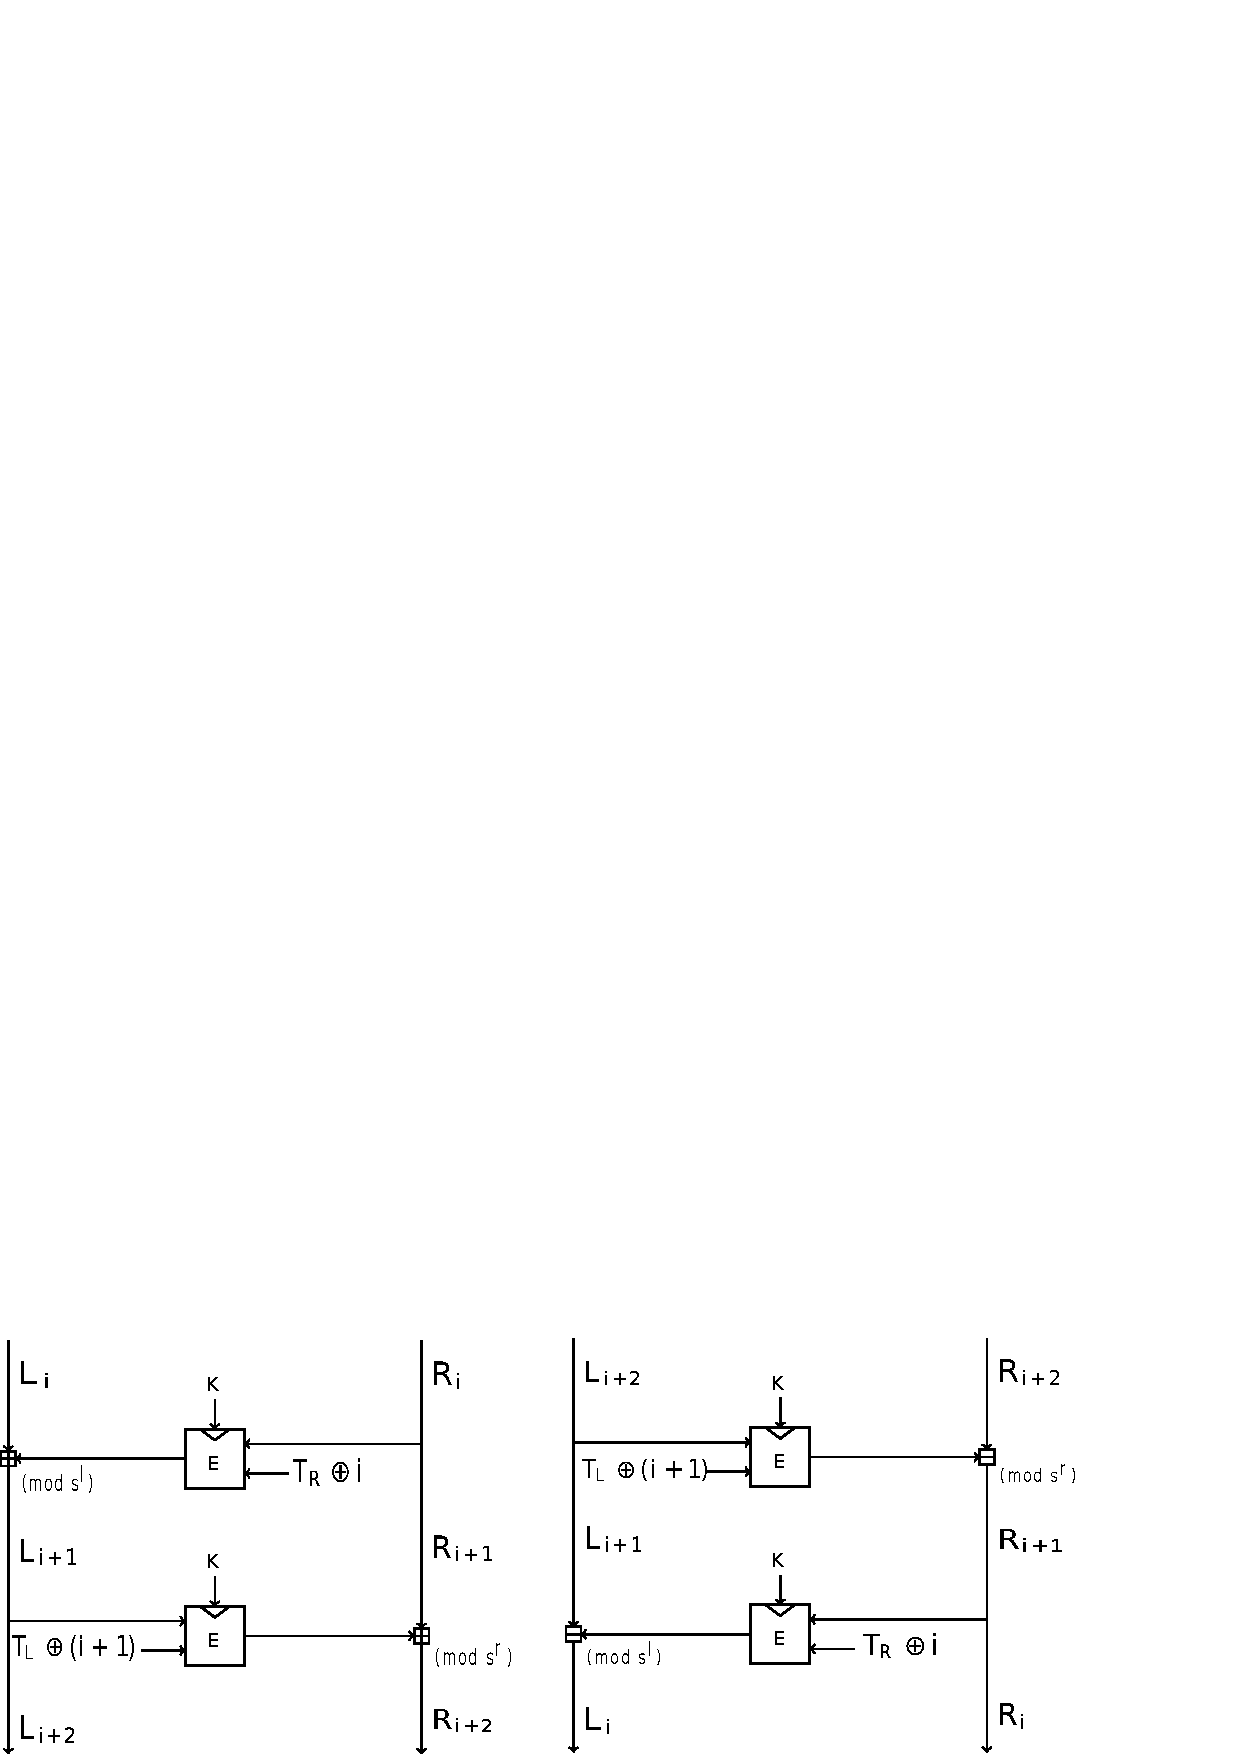
\includegraphics[scale=0.8]{Pictures/BPS_En_De.pdf} 
\caption{Workflow of the internal encryption (Left) and decryption (Right) in the BPS. \cite{BPS}}\label{BPSED}
\center
\end{figure}
\subsection*{Remarks}
\begin{itemize}
\item One advantage of BPS is its adaptability, all the block cipher and hash
function standardized primitives (TDES, AES or SHA-2) can be used as basic internal bricks \cite{BPS}. 
\item The internal tweak values is useful to avoid some kind of dictionary attacks \cite{BPS}. Indeed, if no tweak is used, a third party could build a dictionary of plaintext / ciphertext pairs and find with good probability the eavesdropped encrypted PANs (Personal Account Numbers), this attack works when the amount of data is small, which is particularly the case for an array of numbers encryption \cite{BPS}. "Using random tweak will render this dictionary technique useless as one dictionary per tweak value would be required" \cite{BPS}.
\item An essential quality of BPS is its efficiency. Due to that the input key for all the block cipher internal calls is constant, this requires only one internal cipher key per BPS encryption, which saves a lot of operations and time \cite{BPS}. Moreover, w = 8 rounds is recommanded, it makes the whole encryption process very efficient \cite{BPS}.
\end{itemize}
%%%%%%%%%%%%%%%%%%%%%%%%%%%%%%%%%%%%%%%%%%%%%%%%%%%%%%%%%
%%%%%%%%%%%%%%%%%%%%%%%%%%%%%%%%%%%%%%%%%%%%%%%%%%%%%%%%%
\section{Cipher Feedback Mode (CFB)}\label{CipherFeedbackMode}
\subsubsection*{Package: Crypto.Symmetric.Mode.CFB}
The cipher feedback (CFB) mode, a close relative of CBC, makes a block cipher into a self-synchronizing stream cipher \cite{DBLP:reference/crypt/2011}.
\begin{figure}[htp]
\center
\includegraphics[scale=0.8]{Pictures/CFB_En.pdf} 
\caption{Workflow of the CFB encryption. Adapted from \cite{DBLP:reference/crypt/2011}.}\label{CFBEN}
\center
\end{figure}\\
\subsubsection*{Encryption}
Mathematical description : $C_i=E_K(C_{i-1})\oplus P_i$, $C_0=IV$.\\
Figure \ref{CFBEN} shows the workflow of encryption in CFB. By initialization the start value IV will be stored as $C_0$. To encrypt a $n$ bit ($n<$ Block'Size) message, it will be copied in the plaintext block, and then padded with zeros. To encrypt a plaintext block $P_1$, the start value $C_0$ will be encrypted at first, and then XORed with $P_1$ and stored as $C_1$. Following plaintext blocks will be processed iteratively until the complete message is encrypted.
\subsubsection*{Decryption}
Mathematical description : $P_i=E_K(C_{i-1})\oplus C_i$, $C_0=IV$.\\
As shown in Figure \ref{CFBDE}, the decryption in CFB makes use of the encryption algorithm. At the beginning the mode will be initialized or through \texttt{Set\_IV()} reinitialized. To decrypt a ciphertext block $C_i$, $C_{i-1}$ will be decrypted at first and then XORed with $C_i$. The output of the operation is $P_i$.
\begin{figure}[h]
\centering
\includegraphics[scale=0.8]{Pictures/CFB_De.pdf} 
\caption{Workflow of the CFB decryption. Adapted from \cite{DBLP:reference/crypt/2011}.} \label{CFBDE}
\end{figure}
\subsubsection*{Remarks}
In comparison with CBC-Mode, which can be used when a complete data block exists, CFB-Mode can be used to encrypt not only data but also bytes (8-CFB). Therefore it is mainly used for encryption of byte streams (e.g. Remote shell).\\
In n-CFB-Mode:
\begin{itemize}
\item an error in plaintext will affect the following complete ciphertext and in decryption it goes backward.
\item an error in ciphertext $C_i$ will affect the plaintext block $P_i$ and also the following $\frac{m}{n}-1$ plaintext blocks, where $m$ is the size of the message.
\item An aggressor can change the message bits in the last ciphertext block without being found.
\end{itemize}
%%%%%%%%%%%%%%%%%%%%%%%%%%%%%%%%%%%%%%%%%%%%%%%%%%%%%%%%%
%%%%%%%%%%%%%%%%%%%%%%%%%%%%%%%%%%%%%%%%%%%%%%%%%%%%%%%%%
\section{Counter Mode (CTR)}\label{CounterMode}
\subsubsection*{Package: Crypto.Symmetric.Mode.CTR}
In Counter Mode the feedback isn't dependent on plaintext, but on a counter, which will be increased by 1 after every encryption. Note that the nonce in Figure \ref{CTREN} and Figure \ref{CTRDE} is the same thing as the initial vector (IV) in other graphs. 
\subsubsection*{Encryption}
Mathematical description : $C_i=P_i\oplus E_K(IV+i-1)$.\\
In Figure \ref{CTREN} the counter is initialized at first. The current counter $IV+i-1$ of each block is encrypted, the output is then XORed with plaintext block $P_i$, and the result is $C_i$.
\begin{figure}[h]
\centering
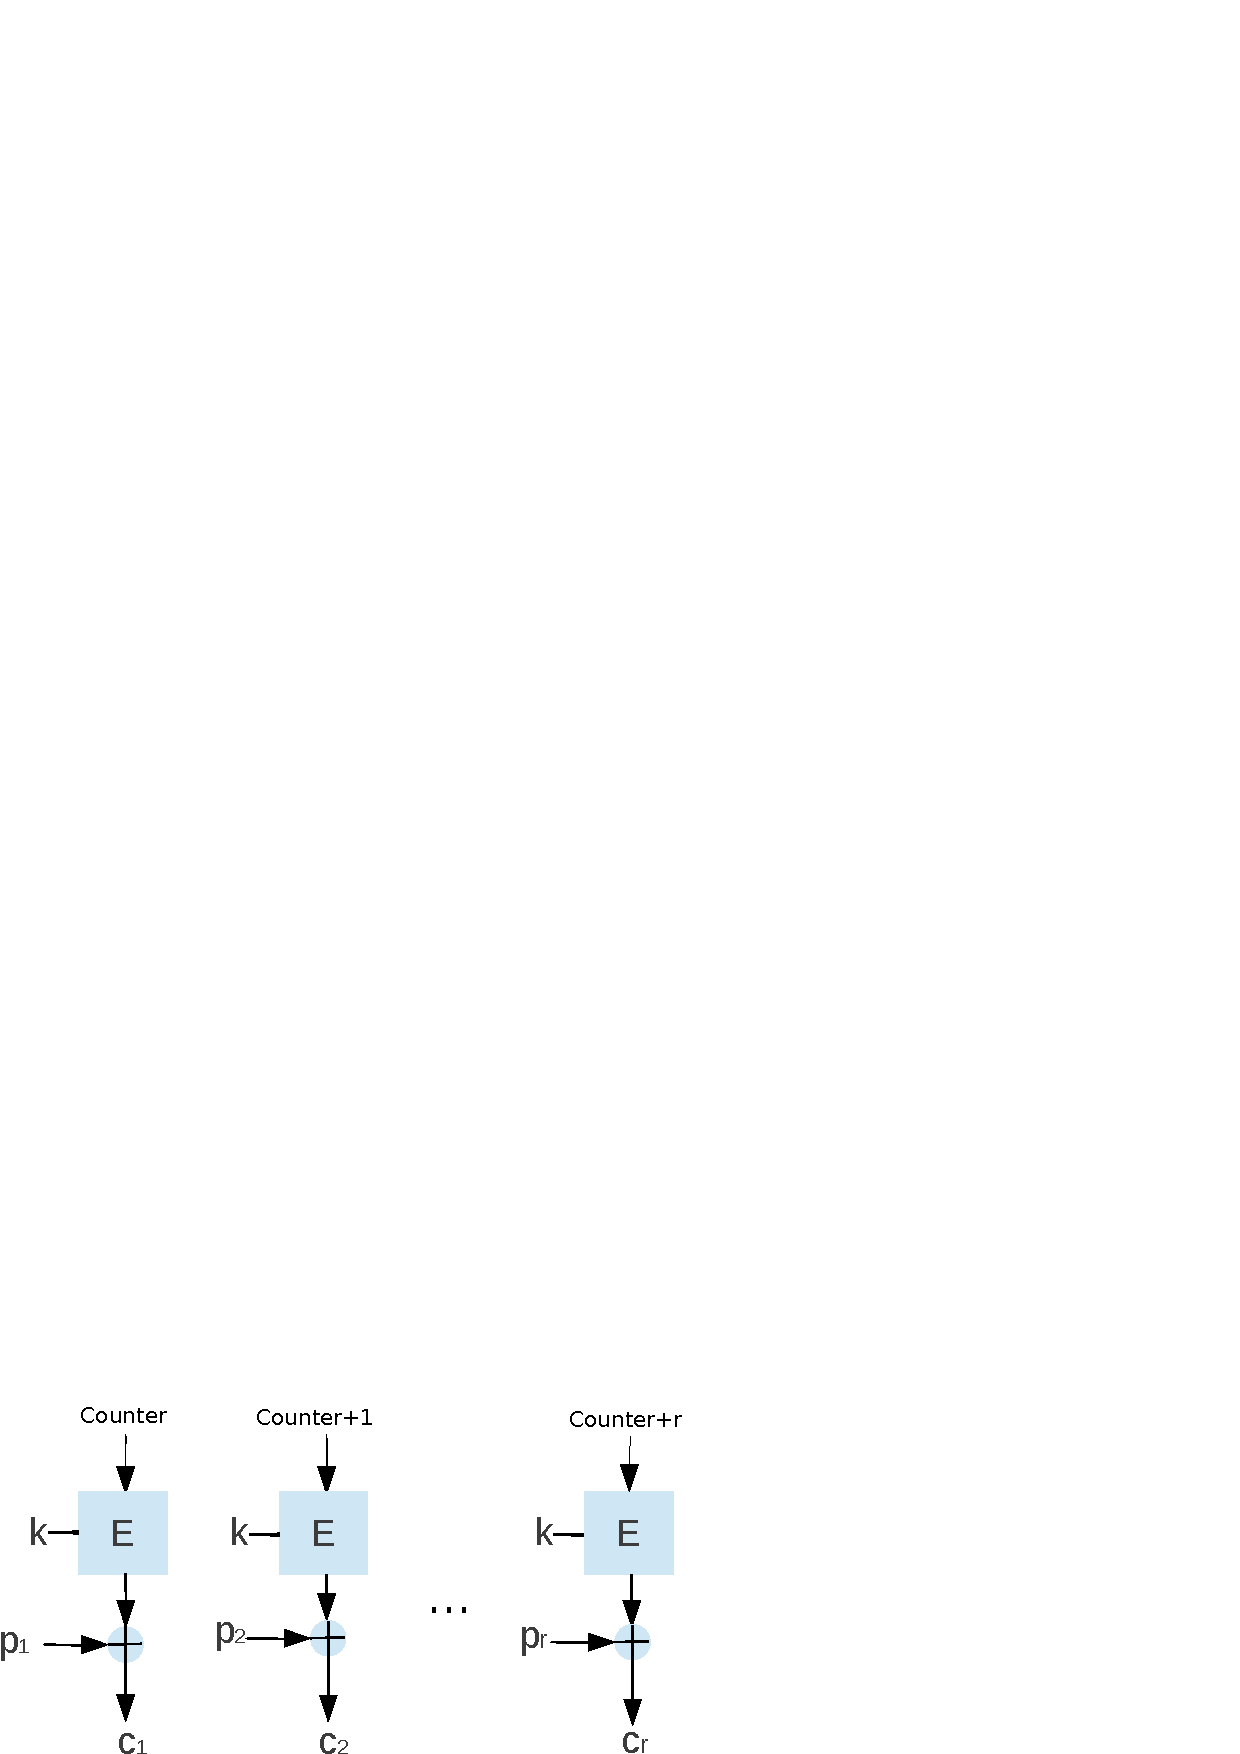
\includegraphics[scale=0.8]{Pictures/CTR_En.pdf} 
\caption{Workflow of the CTR encryption. Adapted from \cite{DBLP:reference/crypt/2011}.}\label{CTREN}
\end{figure}
\subsubsection*{Decryption}
Mathematical description : $P_i=C_i\oplus E_K(IV+i-1)$.\\
Note that in Figure \ref{CTRDE} the encryption algorithm is used in decryption.
After initialization counter $IV+i-1$ will be encrypted, then the output will be XORed with $C_i$ and the result is $P_i$. It is done iteratively until the last block.
\begin{figure}[h]
\centering
\includegraphics[scale=0.8]{Pictures/CTR_De.pdf} 
\caption{Workflow of the CTR decryption. Adapted from \cite{DBLP:reference/crypt/2011}.}\label{CTRDE}
\end{figure}
\subsubsection*{Remarks}
\begin{itemize}
\item \textbf{En-/Decryption of Messages with Random Access}\\
Since that the counter mode is used to decrypt individual ciphertext block, this procedure is suitable for decryption of data with random access e.g. Database.
\item \textbf{Parallel En-/Decryption}\\
Parallelization is possible when man calculates an interval from the start value (IV) and the length of the message is $L$: $[IV\cdots IV+L]$. The interval is decomposed in max. $L$ disjunktive part intervals. Then the message blocks in the part intervals can be en-/decrypted parallel.
\item \textbf{Phasic "High Speed" Encryption}\\
This is a professional function that based on "Low-Level-API" (\ref{Low-Level}) of CTR mode. Please use this only when you konw what it does. In CTR mode it is possible to generate random keystream bits without a message block to be needed. When you generate enough keystream bits with the CTR mode, then you are able to encrypt the messages very quickly through being XORed with the already produced keystream bits.
\end{itemize}
\subsubsection*{Notice:}
\begin{itemize}
\item A bit error in plaintext will influence only one bit in ciphertext and vice versa.
\item Manipulation on plaintext is clear, because every change in ciphertext influences directly the plaintext.
\item Error in Synchronization (Alice and Bob are in different counter states) can not be solved. 
\end{itemize}
\subsubsection*{Low-Level-API}\label{Low-Level}
This API can be used only when you know exactly what it does.
\begin{lstlisting}{}
  procedure Next_Block(Keystream : out Block);
\end{lstlisting}
Mathematical description : $C=E_K(Counter)$; $Counter:=Counter+1$.\\
It encrypts the internal counter to $C$, and the counter will be increased by 1.
%%%%%%%%%%%%%%%%%%%%%%%%%%%%%%%%%%%%%%%%%%%%%%%%%%%%%%%%%%%%%
%%%%%%%%%%%%%%%%%%%%%%%%%%%%%%%%%%%%%%%%%%%%%%%%%%%%%%%%%%%%%
\section{Output Feedback Mode (OFB)}\label{OutputFeedbackMode}
\subsubsection*{Package: Crypto.Symmetric.Mode.OFB}
The OFB mode converts a blockcipher in a stream cipher like the CTR mode. That is, the internal feedback is independent from the plaintext.
\subsubsection*{Encryption}
Mathematical description : $C_i=P_i\oplus K_i\,,\, K_i=E_K(K_{i-1})$.\\
In Figure \ref{OFBEN} shows the workflow of encryption in OFB.
$IV$ is assigned to an internal keystream block $K_0$. Block $K_{i-1}$ will be encrypted to $K_i$ and then XORed with $P_i$, and the result of the operation is ciphertext block $C_i$.
\begin{figure}[h]
\centering
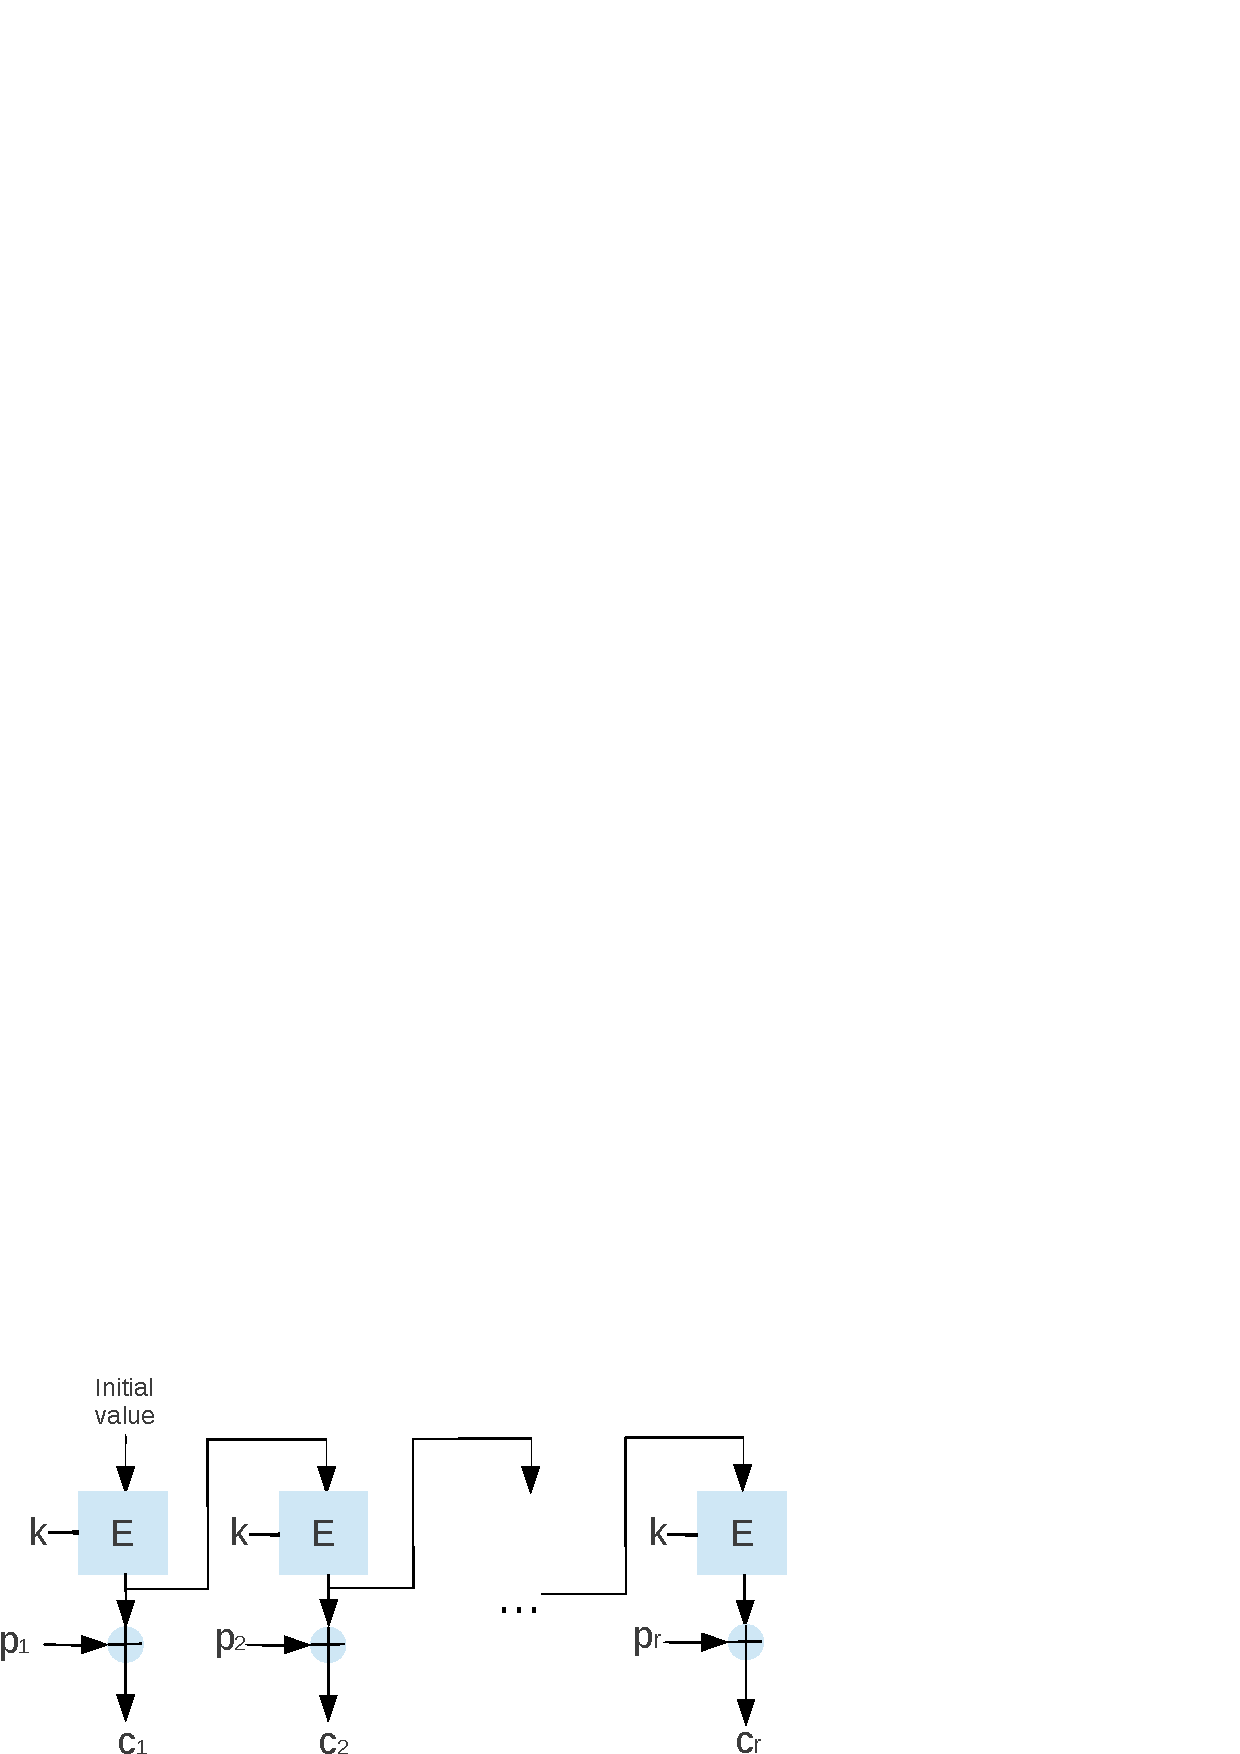
\includegraphics[scale=0.8]{Pictures/OFB_En.pdf} 
\caption{Workflow of the OFB encryption. Adapted from \cite{DBLP:reference/crypt/2011}.}\label{OFBEN}
\end{figure}
\subsubsection*{Decryption}
Mathematical description : $P_i=C_i\oplus K_i\,,\, K_i=E_K(K_{i-1})$.\\
The algorithm encryption is used in decryption as shown in Figure \ref{OFBDE}. The keystream block $K_0$ is initialized with the start value $IV$ or reinitialized by \texttt{Set\_IV()}. $K_{i-1}$ will be encrypted to $K_i$ and XORed with $C_i$. The result of the operation is the plaintext block $P_i$. These ciphertext blocks are decrypted in the same sequence in which they are generated.
\begin{figure}[h]
\centering
\includegraphics[scale=0.8]{Pictures/OFB_De.pdf} 
\caption{Workflow of the OFB decryption. Adapted from \cite{DBLP:reference/crypt/2011}.}\label{OFBDE}
\end{figure}
\subsubsection*{Remarks}
With the "Low-Level-API" (\ref{Low-Level-OFB}) users can generate a keystream without plaintext blocks. Thereby they can encrypt the plaintext blocks very fast. For example it will be possible to generate keystream blocks at night and then encrypt plaintext blocks in the day time. So this mode is very suitable when phasic plaintext blocks should be encrypted quickly.
\subsubsection*{Notice:}
\begin{itemize}
\item The keystream repeats at any time. That is, $\exists L:K_0=K_L$. Supposed $m$ is the block size in bits, then the average length of a cycle goes to $2^m-1$ bits.
\item A bit error in plaintext will influence one bit in ciphertext and vice versa.
\item Manipulation on plaintext is clear, every change in ciphertext influences directly the plaintext.
\item Error in synchronization (Alice and Bob are in different counter states) can not be solved. 
\end{itemize}
\subsubsection*{Low-Level-API}\label{Low-Level-OFB}
The following API can be used only when you know what it does.
\begin{lstlisting}{}
  procedure Next_Block(Keystream : out Block);
\end{lstlisting}
Mathematical description : $K_i=E_K(K_{i-1})$.\\
During initialization the start value IV is stored as keystream block $K_0$. Every time when the \texttt{Next\_Block()} procedure is called, the keystream block $K_i$ will be encrypted to $K_{i+1}$ and resulted as keystream.
%%%%%%%%%%%%%%%%%%%%%%%%%%%%%%%%%%%%%%%%%%%%%%%%%%%%%%%%%%%
%%%%%%%%%%%%%%%%%%%%%%%%%%%%%%%%%%%%%%%%%%%%%%%%%%%%%%%%%%%
\section{Example}
\subsubsection*{CBC Mode}
\begin{lstlisting}{}
  with Crypto.Types;
  with Ada.Text_IO;
  with Crypto.Symmetric.Blockcipher_Tripledes;
  with Crypto.Symmetric.Mode.CBC;
  procedure Example_CBC_Mode is
	 use Ada.Text_IO; use Crypto.Types;
    package TDES renames Crypto.Symmetric.Blockcipher_Tripledes;
    -- use TDES in secure CBC mode
    package TDES_CBC is new Crypto.Symmetric.Mode.CBC(TDES);
	 use TDES_CBC;
    Key: B_Block192 := (16#00#, 16#00#, 16#00#, 16#00#, 16#00#, 
                        16#00#, 16#00#, 16#00#, 16#00#, 16#00#, 
                        16#00#, 16#00#, 16#00#, 16#00#, 16#00#, 
                        16#00#, 16#01#, 16#23#, 16#45#, 16#67#, 
                        16#89#, 16#ab#, 16#cd#, 16#ef#);
    IV: B_Block64 := (16#12#, 16#34#, 16#56#, 16#78#,
            	          16#90#, 16#ab#, 16#cd#, 16#ef#);
    --Plaintext
    P_String: String :="Now is the time for all.";
    --Plaintext will be divided in 3*64 bit blocks.
    P: array(1..3) of B_Block64 := 
			(To_B_Block64(To_Bytes(P_String(1..8))),
          To_B_Block64(To_Bytes(P_String(9..16))),
			 To_B_Block64(To_Bytes(P_String(17..24))));
    --Ciphertext
    C: array(0..3) of B_Block64;
    begin
      Init(Key, IV);    --1. Initialization
      C(0):= IV;        --1. Ciphertext block = start value
      for I in P'Range loop
	     Encrypt(P(I),C(I));  --Encryption
      end loop;
      --For decryption the start value will be 
      --reinitialized with the same value.
      Set_IV(C(0));         
      for I in P'Range loop
         Decrypt(C(I),P(I));   --Decryption
         Put(To_String(To_Bytes(P(I))));
      end loop;
  end Example_CBC_Mode;
\end{lstlisting}\\ \ \\
\subsubsection*{BPS Mode}
\begin{lstlisting}{}
  with Crypto.Symmetric.Mode.BPS;
  with Crypto.Symmetric.Blockcipher_AES128;
  with Crypto.Types; use Crypto.Types;
  with Ada.Text_IO; use Ada.Text_IO;
  procedure Example_BPS_Mode is
    package AES128 renames Crypto.Symmetric.Blockcipher_AES128;
    package BPS is new Crypto.Symmetric.Mode.BPS(AES128);
    use BPS;
    Key : B_Block128 := (16#12#, 16#34#, 16#56#, 16#78#,
	  	                 16#90#, 16#ab#, 16#cd#, 16#ef#,
		                 16#12#, 16#34#, 16#56#, 16#78#,
		                 16#90#, 16#ab#, 16#cd#, 16#ef#);
    IV : B_Block64 :=(16#12#, 16#34#, 16#56#, 16#78#,
		                16#90#, 16#ab#, 16#cd#, 16#ef#);
    Plaintext : BPS.Numerals(1..10) := (0,1,2,3,4,5,6,7,8,9);
    Ciphertext, P : BPS.Numerals(1..10);
    Result : Boolean := False;
  begin
    Init(Key, IV);
    Encrypt(Plaintext, Ciphertext);
    Decrypt(Ciphertext, P);
    for I in Plaintext'Range loop
       if Plaintext(I) = P(I) then
          Result := True;
       end if;
    end loop;
    if Result then
       Put_Line("OK");
    else
       Put_Line("Error"); 
    end if;
  end Example_BPS_Mode;
\end{lstlisting}
  \chapter{Crypto.Symmetric.Mode.Oneway}
This generic package works with one-way blockciphers in one-way modes. It integrates a one-way block cipher with a feedback and also some easy operations ($+,xor$). A one-way mode will be initialized with a random start value (Initial Value (IV)). The ciphertext is therefore not only dependent on the used mode, plaintext and key, but also on the random start value. When users encrypt a plaintext twice with the same key in the same mode but different IVs, then they will get different ciphertexts, i.e. a oneway mode encrypts two plaintext blocks $P_1$ and $P_2$ with $P_1=P_2$ to two ciphertext blocks $C_1$ and $C_2$ with overwhelming probability that $C_1\neq C_2$. So that it is now possible to encrypt more messages with the same key.\\
\textbf{Notice: To decrypt a ciphertext the key and start value by encryption are required.} For this reason the start value should be always kept together with the related ciphertext. \textbf{The security of a mode is independent from the familarity of the start value.} Hense, man multiplies usually the start value with the ciphertext as the final output by attaching the ciphertext to the start value ($C'=IV||C$).
%%%%%%%%%%%%%%%%%%%%%%%%%%%%%%%%%%%%%%%%%%%%%%%%%%%%%%%%%%%%%%
%%%%%%%%%%%%%%%%%%%%%%%%%%%%%%%%%%%%%%%%%%%%%%%%%%%%%%%%%%%%%%
\subsubsection*{Remarks}
\begin{itemize}
\item In a oneway mode it goes similarly as in a normal mode. If a normal mode can be used also as a oneway mode, then you should still prefer oneway mode, because it's nimbler.  
\item The API of this package is the same as in normal modes (\ref{API-Mode}).
\item Supported oneway modes:
\begin{itemize}
\item Cipher Feedback Mode (CFB) (\ref{CipherFeedbackMode})
\item Counter Mode (CTR) (\ref{CounterMode})
\item Output Feedback Mode (OFB) (\ref{OutputFeedbackMode})
\end{itemize}
\end{itemize}
\subsubsection*{Example}
\begin{lstlisting}{}
  with Crypto.Types;
  with Ada.Text_IO;
  with Crypto.Symmetric.Oneway_Blockcipher_Twofish128;
  with Crypto.Symmetric.Mode.Oneway_CTR;
  procedure Example_Mode_Oneway is
	 use Ada.Text_IO; use Crypto.Types;
    package TF128 renames 
                  Crypto.Symmetric.Oneway_Blockcipher_Twofish128;
    package Twofish128 is new
                  Crypto.Symmetric.Mode.Oneway_CTR(TF128);
 	 use Twofish128;
    Key: B_Block128 := (16#2b#, 16#7e#, 16#15#, 16#16#, 16#28#,
                        16#ae#, 16#d2#, 16#a6#, 16#ab#, 16#f7#,
                        16#15#, 16#88#, 16#09#, 16#cf#, 16#4f#,
                        16#3c#);
    IV: B_Block128 := (15 => 1, others => 0);
     --Plaintext
    P_String: String :="All your base are belong to us! ";
     --Plaintext will be divided in 2*64 bit blocks.
    P: array(1..2) of B_Block128 := 
			(To_B_Block128(To_Bytes(P_String(1..16))),
			 To_B_Block128(To_Bytes(P_String(17..32))));
    C: array(0..2) of B_Block128;      --Ciphertext
  begin
    Init(Key, IV);         --Initialization
    C(0):= IV;             --1. Ciphertext block = start value
    for I in P'Range loop
	    Encrypt(P(I),C(I));   --Encryption
    end loop;
     --For decryption the start value will be reinitialized.
    Set_IV(C(0));
    for I in P'Range loop
	    Decrypt(C(I),P(I));     --Decryption
       Put(To_String(To_Bytes(P(I))));
    end loop;
  end Example_Mode_Oneway;
\end{lstlisting}
  \chapter{Crypto.Hashfunction}\label{hash}
Mit Hilfe dieses generischen Paketes l�sst sich aus dem Algorithmus einer
kryptographsichen Hashfunktion (siehe Kapitel \ref{algoh})
eine krypto. Hashfunktion erstellen die sich hervorragend f�r folgende Zwecke 
einsetzen:
\begin{itemize}
\item Integrit�ts�berpr�fung von Nachrichten
\item Generierung und Verifizierung von digitalen Signaturen.
\item Generierung von Zufallszahlen bzw. Zufallsbits
\end{itemize}
Der Zweck dieses Paketes ist es die API f�r Hashfunktionen zu vereintheilichen
und zu vereinfachen. Aus Sicht der Sicherheit spricht hier nichst dagegen 
direkt die native API aus \texttt{Crypto.Symmetric.Algorithm} zu verwenden.\\

%%%%%%%%%%%%%%%%%%%%%%%%%%%%%%%%%%%%%%%%%%%%%%%%%%%%%%%%%%%%%%%%%%%%%%%%%%%%
%%%%%%%%%%%%%%%%%%%%%%%%%%%%%%%%%%%%%%%%%%%%%%%%%%%%%%%%%%%%%%%%%%%%%%%%%%%%

\section{Generischer Teil}
 \begin{lstlisting}{}
generic
   type Hash_Type                 is private;
   type Message_Type              is private;
   type Message_Block_Length_Type is private;
   
   with procedure Init(Hash_Value : out Hash_Type) is <>;

   with procedure Round(Message_Block : in     Message_Type;
                        Hash_Value    : in out Hash_Type) is <>;

   with function Final_Round(Last_Message_Block  : Message_Type;
                             Last_Message_Length :
                             Message_Block_Length_Type;
                             Hash_Value          : Hash_Type)
                             return Hash_Type is <>;

   with procedure Hash(Message    : in Bytes;
                       Hash_Value : out  Hash_Type) is <>;

   with procedure Hash(Message    : in String;
                       Hash_Value : out  Hash_Type) is <>;

   with procedure F_Hash(Filename : in String;
                         Hash_Value : out  Hash_Type) is <>;

 \end{lstlisting}\ \\

%%%%%%%%%%%%%%%%%%%%%%%%%%%%%%%%%%%%%%%%%%%%%%%%%%%%%%%%%%%%%%%%%%%%%%%%%%%
%%%%%%%%%%%%%%%%%%%%%%%%%%%%%%%%%%%%%%%%%%%%%%%%%%%%%%%%%%%%%%%%%%%%%%%%%%%

\section{API}
Die API einer generischen Hashfunktion besteht aus einer High- und einer 
Low-Level-API. Die Low-Level-API sollen sie nur verwenden, wenn sie sich mit
krptographischen Hashfunktionen auskennen. Wenn dies nicht der Fall ist, dann
verwenden sie bitte die folgende High-Level-API.

\subsection{High-Level-API}
\begin{lstlisting}{}
  function Hash  (Message  : Bytes)  return Hash_Type;
  function Hash  (Message  : String) return Hash_Type;
  
  function F_Hash(Filename : String) return Hash_Type;
\end{lstlisting}
Die Funktion \textbf{Hash} liefert den Hashwert einer Nachricht 
(\textit{Message}). Bei der Nachricht kann es sich dabei entweder um ein 
Byte-Array oder einen String handeln. Die Funktion \textbf{F\_Hash} gibt den 
Hashwert der Datei \textit{Filename} zur�ck.  Beispielsweise liefert 
die Codezeile
\begin{lstlisting}{}
  H := F_Hash("/bin/ls")
\end{lstlisting}
den Hashwert von \texttt{/bin/ls}.\\ \ \\


\subsection{Low-Level-API}
Die Low-Level-API besteht aus einer Funktion und zwei Prozeduren. 

\begin{itemize}
\item Die Prozedur \textbf{Init} initialisiert bzw. reinitailisert die 
  Hashfunktion. Jedesmal wenn eine Nachricht gehashed werde soll muss 
  zun�chst diese Prozedure aufgerufen werden.
  \begin{lstlisting}{}
 procedure Init;
  \end{lstlisting}

\item Mit der Prozedure \textbf{Round}, k�nnen iterativ Nachrichtenbl�cke
  gehashed werden. 
  \begin{lstlisting}{}
procedure Round(Message_Block : in Message_Type);
 \end{lstlisting}
 
\item Die Funktion \textbf{Final\_Round} padded und hashed anschlie�end einen
  Nachrichtenblock \textit{Last\_Message\_Block}. Auf Grund des Paddings muss
  die Bytel�nge des Nachrichtenmaterials \textit{Last\_Message\_Length} 
  angegeben werden.  Denn eine Nachricht ist i.d.R.  k�rzer als eine 
  Nachrichtenblock vom Typ \textit{Message\_Type}. Der R�ckgabewert dieser 
  Funktion entspricht dem finalen Hashwert einer Nachricht.
   \begin{lstlisting}{}
function Final_Round(Last_Message_Block  : Message_Type;
                     Last_Message_Length : Message_Block_Length_Type)
                     return Hash_Type;
  \end{lstlisting}
\end{itemize}\ \\

%%%%%%%%%%%%%%%%%%%%%%%%%%%%%%%%%%%%%%%%%%%%%%%%%%%%%%%%%%%%%%%%%%%%%%%%%%%
%%%%%%%%%%%%%%%%%%%%%%%%%%%%%%%%%%%%%%%%%%%%%%%%%%%%%%%%%%%%%%%%%%%%%%%%%%%
%%%%%%%%%%%%%%%%%%%%%%%%%%%%%%%%%%%%%%%%%%%%%%%%%%%%%%%%%%%%%%%%%%%%%%%%%%%

\section{Anwendungsbeispiel}
\subsection{High-Level-API}
Das folgende Beispiel gibt den SHA-256 Hashwert von \textbf{/bin/ls} aus.
 \begin{lstlisting}{}
with Ada.Text_IO;
with Crypto.Types,
with Crypto.Hashfunction_SHA256;


use Crypto.Types, Ada.Text_IO;

procedure example is
   package SHA256 renames Crypto.Hashfunction_SHA256;

   Hash : W_Block256 := SHA256.F_Hash("/bin/ls");
begin
   for I in Hash'Range loop
      Put(To_Hex(Hash(I)));
   end loop;
   Put_Line(" /bin/ls");
end example;
 \end{lstlisting}

\pagebreak

\subsection{Low-Level-API}
\begin{lstlisting}{}
with Ada.Text_IO;
with Crypto.Types;
with Crypto.Hashfunction;
with Crypto.Symmetric.Algorithm.SHA256;

use Ada.Text_IO;
use Crypto.Types;
use Crypto.Symmetric.Algorithm.SHA256;

pragma Elaborate_All (Crypto.Hashfunction);

procedure Example_Hashing is
   package WIO is new  Ada.Text_IO.Modular_IO(Word);

    package SHA256 is
      new Crypto.Hashfunction(Hash_Type    => W_Block256,
                              Message_Type => W_Block512,
                              Message_Block_Length_Type =>
                              Crypto.Types.Message_Block_Length512);

   Message : String :=  "All your base are belong to us!";

   W : Words := To_Words(To_Bytes(Message));

   M : W_Block512 := (others => 0);
   H : W_Block256;
begin
   M(W'Range) := W;

   SHA256.Init;

   -- Berechne den Hashwert von Message
   H := SHA256.Final_Round(M, Message'Last);

   -- Gib den Hashwert von Message aus
   for I in W_Block256'Range loop
      WIO.Put(H(I), Base => 16);
      New_line;
   end loop;
   New_Line;
end Example_Hashing;
\end{lstlisting}

\pagebreak

\section{Anmerkung}
Sie m�ssen nicht jedes mal von neuem aus einem daf�r vorgesehenen symmetrischen
Algorithmus eine Hashfunktion generieren. Stattdessen k�nnen Sie auch eine der 
vorgefertigten Hashfunktionen verwenden.
\begin{itemize}
\item Crypto.Hashfunktion\_SHA1
\item Crypto.Hashfunktion\_SHA256
\item Crypto.Hashfunktion\_SHA512
\item Crypto.Hashfunktion\_Whirlpool
\end{itemize}



  \chapter{Crypto.Symmetric.MAC}\label{MAC}
A message authentication code (MAC) ensures the integrity of a message and sender authentication. It uses a symmetric key (RMAC uses two symmetric keys). The result of the MAC is named an authentication tag. The developer of this library marks it as a (digital) stamp. Three MACs are provided in the ACL, they are randomized MAC (RMAC), hash function based MAC (HMAC) and cipher-based MAC (CMAC).
\section{Randomized MAC (RMAC)}
RMAC is developed by Eliane Jaulmes, Antoine Joux and Frederic Valette. It is based on CBC-MAC and one-way block cipher (Chapter \ref{Oneway-Blockcipher}). It is proved save against the birthday attack. Two keys are required in RMAC.\\
Mathematical description: $RMAC_{K_1,K_2}(E,M)=E_{K_2\oplus R}(C_n)$\,, with $C_i=E_{K_1}(M_i\oplus C_{i-1})$, $R\in_R\{0,1\}^{|K_1|}$ and $C_0=0^n$.
\subsubsection*{Generic Part}
\begin{lstlisting}{}
  generic
    with package C is new 
    					Crypto.Symmetric.Oneway_Blockcipher(<>);
    with procedure Read (Random : out C.Key_Type) is <>;
    with function "xor" (Left, Right : C.Block) return C.Block is <>;
    with function "xor" (Left, Right : C.Key_type) 
     							return C.Key_Type is <>;
\end{lstlisting}
\newpage
\subsubsection*{High-Level-API}
\begin{lstlisting}{}
  type Blocks  is array (Integer range <>) of Block;
  procedure Sign(Message    : in Blocks;
                 Key1, Key2 : in Key_Type;
                 R          : out Key_Type;
                 Tag        : out Block);
  function Verify(Message    : in Blocks;
                  Key1, Key2 : in Key_Type;
                  R          : in Key_Type;
                  Tag        : in Block)  return Boolean;
\end{lstlisting}\\
The procedure \texttt{Sign()} signs \texttt{Message} with two keys, Key1 and Key2. The message is delivered as an array of blocks. Key1 is used to encrypt the whole message blocks, and Key2 is used to generate the final tag based on the calculated ciphertext.
The function \texttt{Verify()} returns true if the term \texttt{Tag} is a valid stamp, otherwise it returns false. When one or more parameters don't agree with those generated from the procedure \texttt{Sign()}, then the function returns false with a significant probability.\\
\subsubsection*{Low-Level-API}
\begin{lstlisting}{}
  procedure Init(Key1, Key2    : in Key_Type);
  procedure Sign(Message_Block : in Block);
  procedure Final_Sign(Final_Message_Block : in Block;
                       R    : out Key_Type;
                       Tag  : out Block);
  procedure Verify(Message_Block : in Block);
  function Final_Verify(Final_Message_Block : in Block;
                        R   : in Key_Type;
                        Tag : in Block)   return Boolean;
\end{lstlisting}
\begin{itemize}
\item The procedure \texttt{Init()} initializes RMAC with two keys, and sets an internal initial state.
\item The procedure \texttt{Sign()} encrypts a message block (\texttt{Message\_Block}). Every time it works only on one block, if there are blocks more than one, the procedure should be called til the last block.
\item The procedure \texttt{Final\_Sign()} encrypts the last message block \texttt{Final\_Message\_Block}, and then generates a random number $R$ to calculates the stamp $Tag$, and finally resets RMAC.
\item The procedure \texttt{Verify()} encrypts a message block (\texttt{Message\_Block}). Every time it works only on one block.
\item The function \texttt{Final\_Verify()} decrypts the last message block \texttt{Final\_Message\_Block}, calculates a new tag and then compares the tag with the delivered one to test if it is valid. True is returned if valid, otherwise false.
\end{itemize}
\subsubsection*{Example}
\begin{lstlisting}{}
  with Crypto.Types; use Crypto.Types;
  with Ada.Text_IO; use Ada.Text_IO;
  with Crypto.Types.Random; use Crypto.Types.Random;
  with Crypto.Symmetric.MAC.RMAC;
  with Crypto.Symmetric.Oneway_Blockcipher_AES128;
  pragma Elaborate_All(Crypto.Symmetric.MAC.RMAC);
  procedure Example_RMAC is
   package AES128 renames Crypto.Symmetric.Oneway_Blockcipher_AES128;
    package RMAC128 is new Crypto.Symmetric.MAC.RMAC(AES128);
    use RMAC128;
    Key1: B_Block128:= (16#00#, 16#01#, 16#02#, 16#03#, 16#04#,
                        16#05#, 16#06#, 16#07#, 16#08#, 16#09#,
                        16#0a#, 16#0b#, 16#0c#, 16#0d#, 16#0e#, 
                        16#0f#);
    Key2 : B_Block128:=(16#00#, 16#11#, 16#22#, 16#33#, 16#44#,
                        16#55#, 16#66#, 16#77#, 16#88#, 16#99#,
                        16#aa#, 16#bb#, 16#cc#, 16#dd#, 16#ee#, 
                        16#ff#);
    R, Tag : B_Block128;
    M : String :="All your base are belong to us! ";
    Message : RMAC128.Blocks(0..1) := 
                        (To_B_Block128(To_Bytes(M(1..16))),		
                         To_B_Block128(To_Bytes(M(17..32))));
  begin
     -- Low-Level
    Init(Key1, Key2);
  	 Sign(Message(0));
  	 Final_Sign(Message(1), R, Tag);
 	 Init(Key1, Key2);
  	 Verify(Message(0));
  	 Put_Line(Final_Verify(Message(1), R, Tag)'Img);
  end Example_RMAC;
\end{lstlisting}
\section{Hash-based MAC (HMAC)}
The designers of HMAC are Mihir Bellare, Ran Canettiy and Hugo Krawczykz. It is based on a hash function. In addition, HMAC\_SHA1, HMAC\_SHA256, HMAC\_512 and HMAC\_Whir\-lpool are available.\\
Mathematical description: $HMAC_K(H,M)=H(K\oplus opad,H((K\oplus ipad)||M))$\,, with $opad=\{0x5C\}^n$ and $ipad=\{0x36\}^n$.
\subsubsection*{Generic Part}
\begin{lstlisting}{}
  generic
    with package H is new Crypto.Symmetric.Hashfunction(<>);
    with function "xor"(Left, Right : H.Message_Type) 
      					          return H.Message_Type is <>;
    with procedure Fill36 (Ipad : out  H.Message_Type) is <>;
    with procedure Fill5C (Opad : out  H.Message_Type) is <>;
    with procedure Copy (Source : in  H.Hash_Type; 
      					    Dest   : out H.Message_Type) is <>;
\end{lstlisting}

The two procedures \texttt{Fill36()} and \texttt{Fill5C()} make the outer/inner padding with value $0x36$ or $0x5C$.
The procedure \texttt{Copy()} copies the content of \texttt{Source} to \texttt{Dest}. If the size of the source value is smaller than that of the destination value, then the rest will be padded with zeros.
All these helping operations are defined in \texttt{Crypto.Symmetric.MAC}.\\
\subsubsection*{API}
\begin{lstlisting}{}
  procedure Init(Key : in Message_Type);
  procedure Sign(Message_Block : in Message_Type);
  procedure Final_Sign
      (Final_Message_Block        : in Message_Type;
       Final_Message_Block_Length : in Message_Block_Length_Type;
       Tag                        : out Hash_Type);
  procedure Verify(Message_Block : in Message_Type);
  function Final_Verify
      (Final_Message_Block        : Message_Type;
       Final_Message_Block_Length : Message_Block_Length_Type;
       Tag                        : Hash_Type) return Boolean;
\end{lstlisting}
\begin{itemize}
\item Procedure \texttt{Init()} initializes the \texttt{HMAC} with the key and sets an initial state.
\item Procedure \texttt{Sign()} hashs a message block (\texttt{Message\_Block}). It is called until to the second to last block.
\item Procedure \texttt{Final\_Sign()} hashs the last message block of the length \texttt{Final\_Message\_B\-lock\_Length}, returns a digital stamp tag and resets the HMAC.
\item Procedure \texttt{Verify()} hashs a message block.
\item The function \texttt{Final\_Verify()} hashs the last message block of the length \texttt{Final\_Message\_B\-lock\_Length}, then verifies whether the tag is valid or not. It returns true if valid, else false.
\end{itemize}
\subsubsection*{Example}
\begin{lstlisting}{}
  with Crypto.Types;
  with Ada.Text_IO;
  with Crypto.Symmetric.MAC;
  with Crypto.Symmetric.MAC.HMAC;
  with Crypto.Symmetric.Hashfunction_SHA256;
  use Crypto.Types;
  use Ada.Text_IO;
  pragma Elaborate_All(Crypto.Symmetric.MAC.HMAC);
  procedure Example_HMAC is
    package HMAC256 is new Crypto.Symmetric.MAC.HMAC
				      (H =>Crypto.Symmetric.Hashfunction_SHA256,
		    		 	 Copy =>Crypto.Symmetric.MAC.Copy,
						 Fill36 =>Crypto.Symmetric.MAC.Fill36,
						 Fill5C =>Crypto.Symmetric.MAC.Fill5C);
    use HMAC256;
    Key : W_Block512 :=(0 => 16#0b0b0b0b#, 1 => 16#0b0b0b0b#,
		                  2 => 16#0b0b0b0b#, 3 => 16#0b0b0b0b#,
		                  4 => 16#0b0b0b0b#, others => 0);
    Message : W_Block512 :=(0 => 16#48692054#, 
    								 1 => 16#68657265#, others => 0);
    Tag : W_Block256;
  begin
    Init(Key);
    Final_Sign(Message, 8, Tag);
    Put_Line(Final_Verify(Message, 8, Tag)'Img);
  end Example_HMAC;
\end{lstlisting}
\subsection*{Remark:}
The users don't need to generate a new HMAC every time. There are already HMACs defined in the ACL.
\begin{itemize}
\item \texttt{Crypto.Symmetric.Mac.Hmac\_SHA1}
\item \texttt{Crypto.Symmetric.Mac.Hmac\_SHA256}
\item \texttt{Crypto.Symmetric.Mac.Hmac\_SHA512}
\item \texttt{Crypto.Symmetric.Mac.Hmac\_Whirlpool}
\end{itemize}
\section{Cipher-based MAC (CMAC)}
CMAC is a blockcipher-based message authentication code. It is used to assure authenticity and integrity of the data.
CMAC is a OMAC1 described in \cite{DBLP:conf/fse/2003}. As shown in Figure \ref{OMAC}, the message is devided into blocks $m_1,m_2,\cdots,m_r$\,, and the first $r-1$ blocks will be processed in a signature algorithm iteratively. The intermediate values are $t_1,t_2,\cdots, t_{r-1}$. Each round can be described mathematically as:
\begin{equation*}
t_i=E_k(t_{i-1}\oplus m_i), \quad 1\leq i \leq r-1\,,\,\mbox{and $t_0$ is a zero block}\,.
\end{equation*}
For the last message block, if it is a full block, then:
\begin{equation*}
Tag=E_k(t_{r-1}\oplus m_r \oplus U)\,,
\end{equation*}
if the block is not a full block, then it will be padded with a one bit and zero bits until it is full, and then:
\begin{equation*}
Tag=E_k(t_{r-1}\oplus m_r \oplus U_2)\,.
\end{equation*}
The terms $U$ and $U_2$ are two non-zero constants based on $L$ in the Galois
field $GF(2^n)$, where $L=E_k(0^n)$. A function is used to calculate $U$ from $L$, and $U_2$ from $U$. It is satisfied that $U\neq U_2$, otherwise, for a full block $m=m'10^*$ and a not full block $m'$, after padding the second block becomes $m'10^*$, they will lead to two identical tags, which is against our design purpose.
Details about this function can be found in \cite{DBLP:conf/fse/2003}.
\begin{figure}[h]
\centering
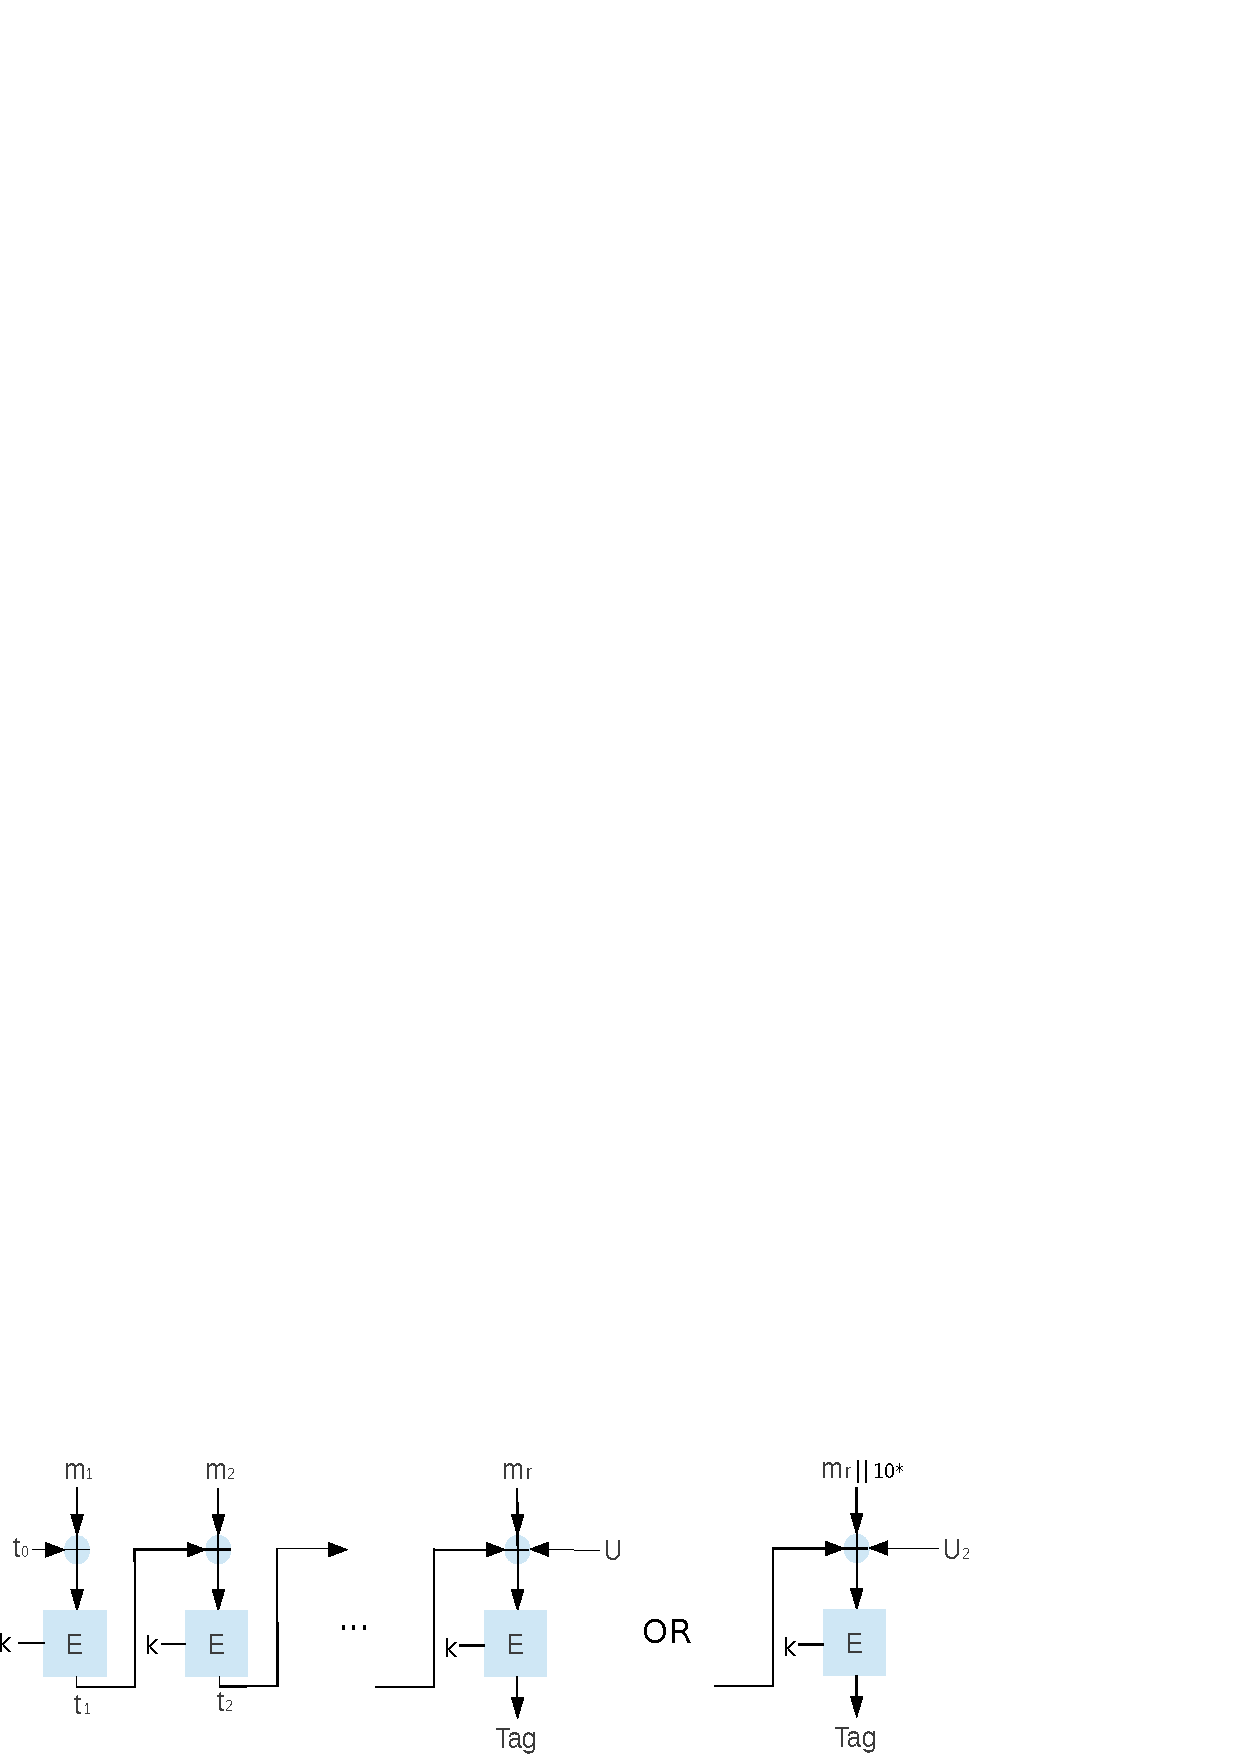
\includegraphics[scale=0.8]{Pictures/CMAC.pdf} 
\caption{The workflow of the CMAC.}\label{OMAC}
\end{figure}
\newpage
\subsubsection*{Generic Part}
\begin{lstlisting}{}
  generic
   with package C is new 
   					Crypto.Symmetric.Oneway_Blockcipher(<>);
   with function To_Block_Type (B : Bytes) return C.Block;
   with function To_Bytes (B : C.Block) return Bytes;
   with function Shift_Left (Value : C.Block; 
   								  Amount: Natural) return C.Block;
   with function "xor" (Left, Right : C.Block) return C.Block is <>;
\end{lstlisting}
\subsubsection*{High-Level-API}
\begin{lstlisting}{}
  type Blocks is array (Integer range <>) of Block;
  procedure Sign(Message : in  Blocks;
                 Key     : in  Key_Type;
                 Tag     : out Block);
  function Verify(Message : in Blocks;
                  Key     : in Key_Type;
                  Tag     : in Block) return Boolean;
\end{lstlisting}
Procedures and functions of high-level use the functions in low-level. Users should always use the high-level interfaces. The message is signed block by block calling internally low-level functions. The function \texttt{Verify()} returns true if the newly created tag equals the delivered tag, else false is returned.\\
\textbf{Exception:} The terms $U$ and $U_2$ (as marked in Figure \ref{OMAC}) are designed in 8 bytes or 16 bytes, which depends on the block size. If the block size is neither 64 bits nor 128 bits:\quad\texttt{Blocklength\_Not\_Supported}.\\
\subsubsection*{Low-Level-API}
\begin{lstlisting}{}
  procedure Init(Key : in Key_Type);
  procedure Sign(Message_Block : in Block);
  procedure Final_Sign(Final_Message_Block : in  Block;
                       Bytes_Read          : in  Natural;
                       Tag                 : out Block);
  procedure Verify(Message_Block : in Block);
  function Final_Verify(Final_Message_Block : in Block;
                        Bytes_Read          : in Natural;
                        Tag                 : in Block)
                        return Boolean;
\end{lstlisting}
\begin{itemize}
\item Procedure \texttt{Init()} makes initialization of the CMAC.
\item Procedure \texttt{Sign()} encrypts one message block (\texttt{Message\_Block}).
\item Procedure \texttt{Final\_Sign()} encrypts the last message block \texttt{Final\_Message\_Block}. If \texttt{Bytes\_Read} of the last message block isn't equal $Block'Size/8$, then it makes padding. A tag is generated and the CMAC is reset.
\item Procedure \texttt{Verify()} encrypts a message block. The block is processed as in procedure \texttt{Sign()}.
\item Procedure \texttt{Final\_Verify()} encrypts the last message block, and makes comparison of a newly generated tag with the delivered tag. It returns true if the two tags are equal, else false.
\end{itemize}
\subsection*{Example}
\begin{lstlisting}{}
  with Ada.Text_IO; use Ada.Text_IO;
  with Crypto.Types; use Crypto.Types;
  with Crypto.Symmetric.Oneway_Blockcipher_AES128;
  with Crypto.Symmetric.MAC.CMAC;
  pragma Elaborate_All(Crypto.Symmetric.MAC.CMAC);

  procedure Example_CMAC is
   package AES128 renames Crypto.Symmetric.Oneway_Blockcipher_AES128;
    package CMAC128 is new Crypto.Symmetric.MAC.CMAC(
						C => AES128, To_Block_Type => To_B_Block128,
						To_Bytes => To_Bytes, 
						Shift_Left => Shift_Block_Left, 
						"xor" => "xor");
    use CMAC128;
    Key : B_Block128 := 
             (16#2b#, 16#7e#, 16#15#, 16#16#, 16#28#, 16#ae#,
		       16#d2#, 16#a6#, 16#ab#, 16#f7#, 16#15#, 16#88#,
		       16#09#, 16#cf#, 16#4f#, 16#3c#);
    Message: CMAC128.Blocks(1..1) :=  (1=>(others=>0));
    Tag : B_Block128;
    Tag_New : B_Block128 := 
        (16#bb#, 16#1d#, 16#69#, 16#29#, 16#e9#, 16#59#,
			16#37#, 16#28#, 16#7f#, 16#a3#, 16#7d#, 16#12#,
			16#9b#, 16#75#, 16#67#, 16#46#);
  begin
    Sign(Message, Key, Tag);
    Put_Line(Verify(Message, Key, Tag_New)'Img);
  end Example_CMAC;
\end{lstlisting}


  \chapter{Crypto.Types.Big\_Numbers}
Dieses Paket stellt den generischen Typen \textit{Big\_Unsigned}, mit einem 
ganzen Satz von Prozeduren und Funktionen, zur Verf�gung. Dieser Typ verwendet
intern ein Array das aus k CPU-W�rtern besteht. Dieses Array wird als ein
modularer Typ interpretiert. Aus diesem Grund es ist nur m�glich 
Big\_Unsigneds deren Bitl�nge einem Vielfachem der CPU-Wortl�nge entspricht zu
generieren. Das dieses Paket ohne Zeiger und Inline-Assembler arbeitet, ist
es um ein vielfaches langsamer als z.B. die auf Effizienz optimierte MPI des
GnuPG\cite{gpg}.\\
Dieses Paket basiert auf Jerome Delcourts Big\_Number-Bibliothek\cite{bignum}.
Urspr�nglich sollte  diese Bibliothek an dieser Stelle verwendet werden.
Es stellte sich aber heraus, das diese doch nicht nicht den gew�nschten
Anforderungen entsprach. Aus diesem Grund wurde dieses Paket noch mal komplett
neu geschrieben. Einen wesentlichen Beitrag zu dem derzeitigen Code
trugen die Analyse des Quellcodes von java.math.BigInteger\cite{bigint} und
Bob Debliers beecyrpt\cite{beecrypt} sowie folgende Quellen
\cite{handout, cormen, schneier, wiki, 2004-hankerson} bei.


\subsubsection{Notation}
\begin{itemize}
\item $|X| \hat{=}$ : Bitl�nge von X.
\item $|CPU|$ \quad : L�nge eines CPU-Wortes.\\ 
  (Bei einem n-Bit Prozessor gilt i.d.R. $|CPU|=n$) 
\end{itemize}



%%%%%%%%%%%%%%%%%%%%%%%%%%%%%%%%%%%%%%%%%%%%%%%%%%%%%%%%%%%%%%%%%%%%%%%%%%%

\section{API}

\subsection{Generischer Teil}
\begin{lstlisting}{}
generic
   Size : Positive;
\end{lstlisting}
\textbf{Vorbedingung:}
$Size = k \cdot |CPU| \quad k \in N$\\ \ \\
\textbf{Exception:}
$Size \not= k \cdot |CPU| \quad k \in N$ : Constraint\_Size\_Error.\\ \ \\

Size gibt die Bitl�nge des Types \textit{Big\_Unsigned} an.\\

%%%%%%%%%%%%%%%%%%%%%%%%%%%%%%%%%%%%%%%%%%%%%%%%%%%%%%%%%%%%%%%%%%%%%%%%%%%

\subsection{Typen}\ 

\begin{tabular}{p{\textwidth}}
\begin{lstlisting}{}
  type Big_Unsigned is private;
\end{lstlisting}\\
Dies ist dar Basis-Typ des Paketes. Big\_Unsigned repr�sentiert eine 
modulare n-Bit Zahl. ($n = k\cdot m$ wobei m die L�nge eines CPU-Wortes ist).
Eine Variable von diesem Typ wir immer mit der Konstanten Big\_Unsigned\_Zero
(\ref{buz}) initialisiert.\\ \ \\
 \hline
\end{tabular}

\begin{tabular}{p{\textwidth}}
\begin{lstlisting}{}
   subtype Number_Base is Integer range 2 .. 16;
\end{lstlisting}\\
Dieser Typ wird sp�ter bei der Konvertierung einer Big\_Unsigned in einen 
String ben�tigt. Ein Big\_Unsigned Variable kann nur als eine Zahl zu einer
Basis dieses Types dargestellt werden.\\ \ \\
\hline
\end{tabular}

\begin{tabular}{p{\textwidth}}
\begin{lstlisting}{}
  type Mod_Type is mod 2**System.Word_Size;
   for Mod_Type'Size use System.Word_Size;
\end{lstlisting}\\
Mod\_Type ist ein Modulare Typ der die L�nge eines CPU-Wortes hat. Bei einem
24-Bit Prozessor ist System.Word\_Size = 24 bei einem 32-Bit Prozessor ist
System.Word\_Size = 32 usw.\\ \ \\ \ \\
\end{tabular}

%%%%%%%%%%%%%%%%%%%%%%%%%%%%%%%%%%%%%%%%%%%%%%%%%%%%%%%%%%%%%%%%%%%%%%%%%%%

\subsection{Konstanten}\label{buz}
\begin{lstlisting}{}
 Big_Unsigned_Zero    : constant Big_Unsigned; -- = 0
 Big_Unsigned_One     : constant Big_Unsigned; -- = 1
 Big_Unsigned_Two     : constant Big_Unsigned; -- = 2
 Big_Unsigned_Three   : constant Big_Unsigned; -- = 3
 Big_Unsigned_Four    : constant Big_Unsigned; -- = 4
 Big_Unsigned_Sixteen : constant Big_Unsigned; -- = 16
 Big_Unsigned_First   : constant Big_Unsigned; -- = 0
 Big_Unsigned_Last    : constant Big_Unsigned; -- = "Big_Unsigned'Last"
\end{lstlisting}\ \\ 


%%%%%%%%%%%%%%%%%%%%%%%%%%%%%%%%%%%%%%%%%%%%%%%%%%%%%%%%%%%%%%%%%%%%%%%%%%%

\section{Vergleichsoperationen}
\begin{lstlisting}{}
 -- Vergleiche Big_Unsigned mit Big_Unsigned

 function "="(Left, Right : Big_Unsigned) return Boolean;
 function "<"(Left, Right : Big_Unsigned) return Boolean;
 function ">"(Left, Right : Big_Unsigned) return Boolean;

 function "<="(Left, Right : Big_Unsigned) return Boolean;
 function ">="(Left, Right : Big_Unsigned) return Boolean;

 function Min(X, Y : in Big_Unsigned) return Big_Unsigned;
 function Max(X, Y : in Big_Unsigned) return Big_Unsigned;


  -- Vergleiche Big_Unsigned mit Mod_Type

 function "=" (Left  : Big_Unsigned;
               Right : Mod_Type)
               return  Boolean;

 function "=" (Left  : Mod_Type;
               Right : Big_Unsigned) 
	       return  Boolean;

 function "<" (Left  : Big_Unsigned;
               Right : Mod_Type)
               return Boolean;

 function "<" (Left  : Mod_Type;
               Right : Big_Unsigned)
               return  Boolean;

 function ">" (Left  : Big_Unsigned; 
               Right : Mod_Type)
               return  Boolean;

 function ">" (Left  : Mod_Type;
               Right : Big_Unsigned)
               return  Boolean;

 function "<=" (Left  : Big_Unsigned;
                Right : Mod_Type)
                return  Boolean;

 function "<="(Left  : Mod_Type;
               Right : Big_Unsigned)
               return  Boolean;
  
 function ">=" (Left  : Big_Unsigned;
                Right : Mod_Type)
                return  Boolean;

 function ">=" (Left  : Mod_Type; 
                Right : Big_Unsigned) 
                return  Boolean;
\end{lstlisting}\ \\

\subsection{Elementare Operationen}
\begin{lstlisting}{}
function "+" (Left, Right : Big_Unsigned) return Big_Unsigned;

function "+" (Left  : Big_Unsigned;
              Right : Mod_Type) 
              return  Big_Unsigned;

function "+" (Left :  Mod_Type;
              Right : Big_Unsigned)
              return  Big_Unsigned;


function "-" (Left, Right : Big_Unsigned) return Big_Unsigned;

function "-" (Left  : Big_Unsigned;
              Right : Mod_Type)
              return  Big_Unsigned;

function "-" (Left  : Mod_Type;
              Right : Big_Unsigned) 
              return  Big_Unsigned;


function "*" (Left, Right : Big_Unsigned) return Big_Unsigned;

function "*" (Left  : Big_Unsigned; 
              Right : Mod_Type) 
              return  Big_Unsigned;

function "*" (Left  : Mod_Type; 
              Right : Big_Unsigned)
              return  Big_Unsigned;


function "/" (Left, Right : Big_Unsigned) return Big_Unsigned;

function "/" (Left  : Big_Unsigned; 
              Right : Mod_Type)
              return  Big_Unsigned;

function "/" (Left  : Mod_Type; 
              Right : Big_Unsigned)
              return  Big_Unsigned;


function "xor" (Left, Right : Big_Unsigned) return Big_Unsigned;

function "and" (Left, Right : Big_Unsigned) return Big_Unsigned;

function "or"  (Left, Right : Big_Unsigned) return Big_Unsigned;

function "**"  (Left, Right : Big_Unsigned) return Big_Unsigned;

function "mod" (Left, Right : Big_Unsigned) return Big_Unsigned;

function "mod" (Left  : Big_Unsigned;
                Right : Mod_Type) 
                return  Big_Unsigned;
\end{lstlisting} \ \\


\subsubsection{Multiplikation}
Zus�tzlich zu der elementaren Multiplikation wurden noch weitere Algorithmen 
implementiert, die ihr Potential bei gr��eren Zahlen entfalten. Leider lassen
die theoretischen Laufzeiten nicht in der ACL erreichen. Je komplexer die 
Algorithmen werden, desto mehr Rechenoperationen und Variablen werden ben�tigt.
An dieser Stelle l�sst sich der Flaschenhals erkennen, welcher in der 
Initialisierung von \textit{Big\_Unsigned} steckt.\\

Weitere Multiplikationsalgorihmen sind:\\
\begin{tabular}{l}
\hline
\begin{lstlisting}{}
 function Russ        (Left, Right : Big_Unsigned)
                      return Big_Unsigned;
\end{lstlisting}
Die Russische Bauernmultiplikation $O(N^2)$ basierend auf Bitoperationen.\\

\hline
\begin{lstlisting}{}
 function Karatsuba   (Left, Right : Big_Unsigned)
                      return Big_Unsigned;
\end{lstlisting}
Der Karatsuba $ \left(O\left(N^{log_2 3}\right) = O\left(N^{1.585}\right)\right)$ 
Algorithmus teilt die Faktoren intern in Polynome 1. Grades und brechnet die 
Teilprodukte mit der Schulmethode.\\

\hline
\begin{lstlisting}{}
 function Karatsuba_P (Left, Right : Big_Unsigned)
                      return Big_Unsigned;
\end{lstlisting}
Die Berechnung der Teilprodukte wird parallel in Tasksausgef�hrt.\\

\hline
\begin{lstlisting}{}
 function Toom_Cook   (Left, Right : Big_Unsigned)
                      return Big_Unsigned;
\end{lstlisting}
Die hier Implementierte variante ist der Toom-Cook-3-Way 
$\left(O\left(N^{1,465}\right)\right)$ Algorithmus nach D. Knuth. Er teilt die 
Faktoren intern in Polynome 2. Grades und brechnet die 
Teilprodukte mit der Schulmethode.\\

\hline
\begin{lstlisting}{}
 function Toom_Cook_P (Left, Right : Big_Unsigned)
                      return Big_Unsigned;
\end{lstlisting}
Die Berechnung der Teilprodukte wird parallel in Tasksausgef�hrt.\\
\hline
\end{tabular}
Alle Algorithmen lassen sich explizit Aufrufen und zur Multiplikation zweier 
\textit{Big\_Unsigned} benutzen.\\

Eine Performance-Steigerung l�sst sich dennoch durch die Verzahnung
der Algorithmen erreichen, welche versucht die St�rken der
verschiedenen Algorithmen zu kombinieren. Intern ruft dazu der
�berladene Operator \texttt{*} f�r kleine Faktoren die Schulmethode, f�r
gr��ere (ca. 3100 Bit) den parallelen Karatsuba und ab ca. 3900 Bit
L�nge den parallelen Toom-Cook-Algorithmus auf.

%%%%%%%%%%%%%%%%%%%%%%%%%%%%%%%%%%%%%%%%%%%%%%%%%%%%%%%%%%%%%%%%%%%%%%%%%%%
%%%%%%%%%%%%%%%%%%%%%%%%%%%%%%%%%%%%%%%%%%%%%%%%%%%%%%%%%%%%%%%%%%%%%%%%%%%

\section{Utils}
In dem separatem Body Crypto.Types.Big\_Numbers.Utils verbergen sich sehr
viele n�tzliche Funktionen und Prozeduren. Der Zugriff erfolgt �ber das Pr�fix
\textbf{Utils.}\\

\begin{tabular}{p{\textwidth}}
\begin{lstlisting}{}
procedure Swap(X, Y : in out Big_Unsigned);
\end{lstlisting}\\
Diese Prozedur vertauscht \textit{X} mit \textit{Y}.\\ \ \\
\hline
\end{tabular}

%%%%%%%%%%%%%%%%%%%%%%%%%%%%%%%%%%%%%%%%%%%%%%%%%%%%%%%%%%%%%%%%%%%%%%%%%%%

\begin{tabular}{p{\textwidth}}
\begin{lstlisting}{}
procedure Set_Least_Significant_Bit(X : in out Big_Unsigned);
\end{lstlisting}\\
Diese Prozedur setzt das niederwertigste Bit von \textit{X} auf 1.\\
Dadurch ist \textit{X} nach diesem Prozeduraufruf immer ungerade. \\ \ \\
\hline
\end{tabular}

%%%%%%%%%%%%%%%%%%%%%%%%%%%%%%%%%%%%%%%%%%%%%%%%%%%%%%%%%%%%%%%%%%%%%%%%%%%

\begin{tabular}{p{\textwidth}}
\begin{lstlisting}{}
 procedure Set_Most_Significant_Bit(X : in out Big_Unsigned); 
\end{lstlisting}\\
Diese Prozedur setzt das h�chstwertigste Bit von \textit{X} auf 1.\\
Damit ist \textit{X} nach dem Prozeduraufruf eine Size-Bit Zahl.\\ \ \\
\hline
\end{tabular}

%%%%%%%%%%%%%%%%%%%%%%%%%%%%%%%%%%%%%%%%%%%%%%%%%%%%%%%%%%%%%%%%%%%%%%%%%%%

\begin{tabular}{p{\textwidth}}
\begin{lstlisting}{}
  function Is_Odd(X : Big_Unsigned) return Boolean;
\end{lstlisting}\\
Diese Funktion liefert  \textit{True} zur�ck, wenn
\textit{X} ungerade ist, ansonsten \textit{False}.  \\ \ \\
\hline
\end{tabular}

%%%%%%%%%%%%%%%%%%%%%%%%%%%%%%%%%%%%%%%%%%%%%%%%%%%%%%%%%%%%%%%%%%%%%%%%%%%

\begin{tabular}{p{\textwidth}}
\begin{lstlisting}{}
  function Is_Even(X : Big_Unsigned) return Boolean;
\end{lstlisting}\\
Diese Funktion liefert \textit{True} zur�ck, wenn
X gerade ist, ansonsten \textit{False}. \\ \ \\
\hline
\end{tabular}

%%%%%%%%%%%%%%%%%%%%%%%%%%%%%%%%%%%%%%%%%%%%%%%%%%%%%%%%%%%%%%%%%%%%%%%%%%%

\begin{tabular}{p{\textwidth}}
\begin{lstlisting}{}
 procedure Inc(X : in out Big_Unsigned);
\end{lstlisting}\\
Diese Prozedur erh�ht X um 1.\\ \ \\
\hline
\end{tabular}

%%%%%%%%%%%%%%%%%%%%%%%%%%%%%%%%%%%%%%%%%%%%%%%%%%%%%%%%%%%%%%%%%%%%%%%%%%%


\begin{tabular}{p{\textwidth}}
\begin{lstlisting}{}
 procedure Dec(X : in out Big_Unsigned);
\end{lstlisting}\\
Diese Prozedur vermindert X um 1.\\ \ \\
\hline
\end{tabular}

%%%%%%%%%%%%%%%%%%%%%%%%%%%%%%%%%%%%%%%%%%%%%%%%%%%%%%%%%%%%%%%%%%%%%%%%%%%

\begin{tabular}{p{\textwidth}}
\begin{lstlisting}{}
 function Shift_Left (Value  : Big_Unsigned; 
                      Amount : Natural) 
                      return   Big_Unsigned;

\end{lstlisting}\\
Diese Funktion berechnet  $Value * 2^{Amount}$.\\ \ \\
\hline
\end{tabular}

%%%%%%%%%%%%%%%%%%%%%%%%%%%%%%%%%%%%%%%%%%%%%%%%%%%%%%%%%%%%%%%%%%%%%%%%%%%

\begin{tabular}{p{\textwidth}}
\begin{lstlisting}{}
function Shift_Right (Value  : Big_Unsigned; 
                      Amount : Natural)
                      return    Big_Unsigned;
\end{lstlisting}\\
Diese Funktion berechnet  $\lfloor Value / 2^{Amount}\rfloor$.\\ \ \\
\hline
\end{tabular}

%%%%%%%%%%%%%%%%%%%%%%%%%%%%%%%%%%%%%%%%%%%%%%%%%%%%%%%%%%%%%%%%%%%%%%%%%%%


\begin{tabular}{p{\textwidth}}
\begin{lstlisting}{}
function Rotate_Left(Value  : Big_Unsigned;
                     Amount : Natural)
                     return   Big_Unsigned;
\end{lstlisting}\\
Diese Funktion berechnet
$((Value * 2^{Amount})\; \oplus\; (\lfloor Value / 2^{Size - Amount}\rfloor))$
$\bmod\; 2^{Size}$.\\ \ \\
Der eingebene Amount wird als erstes mod size genommen, sodass nachfolgender Code ausgef"uhrt werden kann:
\begin{lstlisting}{}
Shift_Left(Value, Amount) xor Shift_Right(Value,Size - Amount)
\end{lstlisting}
$\bmod\; 2^{Size}$.\\ \ \\

\hline
\end{tabular}

%%%%%%%%%%%%%%%%%%%%%%%%%%%%%%%%%%%%%%%%%%%%%%%%%%%%%%%%%%%%%%%%%%%%%%%%%%%

\begin{tabular}{p{\textwidth}}
  \begin{lstlisting}{}
    function Rotate_Right(Value  : Big_Unsigned; 
    Amount : Natural)
    return   Big_Unsigned;
  \end{lstlisting}\\
  Diese Funktion berechnet
  $((Value * 2^{Size-Amount})\; \oplus\; (\lfloor Value / 2^{Amount}\rfloor))$
  $\bmod\; 2^{Size}$.\\ \ \\
  Der eingebene Amount wird als erstes mod size genommen, sodass nachfolgender Code ausgef"uhrt werden kann:
  \begin{lstlisting}{}
    Shift_Right(Value, Amount) xor Shift_Left(Value,Size - Amount)
  \end{lstlisting}\\
  \hline
\end{tabular}

%%%%%%%%%%%%%%%%%%%%%%%%%%%%%%%%%%%%%%%%%%%%%%%%%%%%%%%%%%%%%%%%%%%%%%%%%%%

\begin{tabular}{p{\textwidth}}
\begin{lstlisting}{}
function Get_Random return Big_Unsigned;
\end{lstlisting}\\
Diese Funktion generierte eine Zufallszahl aus dem Intervall 
\{$0\ldots ,$Big\_Unsigned\_Last\}.\\ \ \\
\hline
\end{tabular}

%%%%%%%%%%%%%%%%%%%%%%%%%%%%%%%%%%%%%%%%%%%%%%%%%%%%%%%%%%%%%%%%%%%%%%%%%%%

\begin{tabular}{p{\textwidth}}
\begin{lstlisting}{}
function Bit_Length(X : Big_Unsigned) return Natural;
\end{lstlisting}\\
Diese Funktion berechnet die Bitl�nge von X.\\ \ \\
\hline
\end{tabular}

%%%%%%%%%%%%%%%%%%%%%%%%%%%%%%%%%%%%%%%%%%%%%%%%%%%%%%%%%%%%%%%%%%%%%%%%%%%

\begin{tabular}{p{\textwidth}}
\begin{lstlisting}{}
function Lowest_Set_Bit(X : Big_Unsigned) return Natural;
\end{lstlisting}\\
Diese Funktion berechnet die Position des niederwertigsten Bits von X, das
den Wert ``1'' hat.\\ \ \\
\textbf{Exception:}\\
$X =$ Big\_Unsigned\_Zero : Is\_Zero\_Error\\ \ \\   
\hline
\end{tabular}

%%%%%%%%%%%%%%%%%%%%%%%%%%%%%%%%%%%%%%%%%%%%%%%%%%%%%%%%%%%%%%%%%%%%%%%%%%%

\begin{tabular}{p{\textwidth}}
\begin{lstlisting}{}
function Gcd(Left, Right : Big_Unsigned) return Big_Unsigned;
\end{lstlisting}\\
Diese Funktion berechnet den gr��ten gemeinsamen Teiler von \textit{Left}
und \textit{Right}.\\ \ \\
\hline
\end{tabular}

%%%%%%%%%%%%%%%%%%%%%%%%%%%%%%%%%%%%%%%%%%%%%%%%%%%%%%%%%%%%%%%%%%%%%%%%%%%

\begin{tabular}{p{\textwidth}}
\begin{lstlisting}{}
function Length_In_Bytes(X : Big_Unsigned) return Natural;
\end{lstlisting}\\
Diese Funktion berechnet die Anzahl der Bytes die man ben�tigt um X als
Byte-Array auszugeben.\\ \ \\
\hline
\end{tabular}

%%%%%%%%%%%%%%%%%%%%%%%%%%%%%%%%%%%%%%%%%%%%%%%%%%%%%%%%%%%%%%%%%%%%%%%%%%%

\begin{tabular}{p{\textwidth}}
\begin{lstlisting}{}
function To_Big_Unsigned(X : Bytes) return Big_Unsigned;
\end{lstlisting}\\
Diese Funktion wandelt ein Byte-Array \textit{X} in eine Big\_Unsigned B um.
Dabei wird X(X'First) zum h�chstwertigstem Byte von B und X(X'Last)
zum niederwertigstem Byte von B.\\ \ \\
\textbf{Exception:}\\
$X'Length * Byte'Size > Size$  : Constraint\_Error\\ \ \\
\hline
\end{tabular}

%%%%%%%%%%%%%%%%%%%%%%%%%%%%%%%%%%%%%%%%%%%%%%%%%%%%%%%%%%%%%%%%%%%%%%%%%%%

\begin{tabular}{p{\textwidth}}
\begin{lstlisting}{}
function To_Bytes(X : Big_Unsigned) return Bytes;
\end{lstlisting}\\
Diese Funktion wandelt \textit{X} in ein Byte-Array B um.
Dabei wird das h�chstwertigste Byte von X zu B(B'First), und das 
niederwertigste Byte von X wird zu B(B'Last).\\ \ \\  
\hline
\end{tabular}

%%%%%%%%%%%%%%%%%%%%%%%%%%%%%%%%%%%%%%%%%%%%%%%%%%%%%%%%%%%%%%%%%%%%%%%%%%%

\begin{tabular}{p{\textwidth}}
\begin{lstlisting}{}
function To_String (Item : Big_Unsigned;
                    Base : Number_Base := 10)
		    return String;
\end{lstlisting}\\
Diese Funktion wandelt \textit{Item} in einen String um. Die Umwandlung 
erfolgt dabei zur Basis \textit{Base} ($Base \in \{2,\ldots ,16\}$)
Der String hat folgenden Aufbau:
\begin{description}
\item[Base=10: ] Einen Zahl zur Basis 10
  (Bsp. ``1325553'')
\item[Base/=10: ] \textit{Base}\# eine Zahl zur Basis B\#
  (Bsp. ``12\#AB45623A3402\#'')
\end{description}\ \\ \ \\
\hline
\end{tabular}

%%%%%%%%%%%%%%%%%%%%%%%%%%%%%%%%%%%%%%%%%%%%%%%%%%%%%%%%%%%%%%%%%%%%%%%%%%%

\begin{tabular}{p{\textwidth}}
\begin{lstlisting}{}
function To_Big_Unsigned(S : String) return Big_Unsigned;
\end{lstlisting}\\
Dies Funktion wandelt eine Zeichenkette \textit{S} in eine Big\_Unsigned um.
Die �bergebene Zeichenkette wird als Zahl in dezimaler Notation oder als 
eine Zahl zur Basis B ($B \in \{2,...,16\}$) betrachtet und muss folgenden
Aufbau haben: 
\begin{itemize}
\item B\#eine Zahl zur Basis B\#
  (Bsp. S = ``16\#FF340A12B1\#'')
\item eine Zahl zur Basis 10 
  (Bsp. S = ``333665'')
\end{itemize} \ \\
\textbf{Exception:}\\
\begin{tabular}{l @{\ :\ } l}
  S ist eine leere Zeichenkette & Conversion\_Error\\
  S hat eine ung�ltige Basis & Conversion\_Error\\
  S hat ung�ltige Ziffern &  Conversion\_Error
\end{tabular}\ \\ \ \\
\hline
\end{tabular}

\begin{tabular}{p{\textwidth}}
\begin{lstlisting}{}
procedure Put (Item : in Big_Unsigned;
               Base : in Number_Base := 10);
\end{lstlisting}\\
Diese Prozedur gibt die Big\_Unsigned \textit{Item} auf der Standardausgabe
zur Basis \textit{Base} ($Base \in \{2,...,16\}$) aus.\\ \ \\ 
\hline
\end{tabular}

%%%%%%%%%%%%%%%%%%%%%%%%%%%%%%%%%%%%%%%%%%%%%%%%%%%%%%%%%%%%%%%%%%%%%%%%%%%

\begin{tabular}{p{\textwidth}}
\begin{lstlisting}{}
procedure Put_Line(Item : in Big_Unsigned;
                   Base : in Number_Base := 10);
\end{lstlisting}\\
Diese Prozedur gibt die Big\_Unsigned \textit{Item} auf der Standardausgabe,
inklusive Zeilenumbruch, zur Basis \textit{Base} 
($Base \in \{2,...,16\}$) aus.\\ \ \\ 
\hline
\end{tabular}

%%%%%%%%%%%%%%%%%%%%%%%%%%%%%%%%%%%%%%%%%%%%%%%%%%%%%%%%%%%%%%%%%%%%%%%%%%%

\begin{tabular}{p{\textwidth}}
\begin{lstlisting}{}
procedure Big_Div (Dividend, Divisor : in Big_Unsigned;
                   Quotient, Remainder : out Big_Unsigned);
\end{lstlisting}\\
Diese Prozedur berechnet den Quotienten \textit{Quotient} und den Rest
\textit{Remainder} einer ganzzahligen Division. Es gilt:
\begin{itemize}
\item $Quotient := \lfloor \frac{Dividend}{Divisor} \rfloor$
\item $Remainder :=  Dividend\; \bmod\; Divisor$
\end{itemize}\ \\
\textbf{Exception:}\\
$X =$ Big\_Unsigned\_Zero : Is\_Zero\_Error\\ \ \\   
\hline
\end{tabular}

%%%%%%%%%%%%%%%%%%%%%%%%%%%%%%%%%%%%%%%%%%%%%%%%%%%%%%%%%%%%%%%%%%%%%%%%%%%


\begin{tabular}{p{\textwidth}}
\begin{lstlisting}{}
procedure Short_Div (Dividend  : in  Big_Unsigned;
                     Divisor   : in  Mod_Type;
                     Quotient  : out Big_Unsigned;
                     Remainder : out Mod_Type);
\end{lstlisting}\\
Diese Prozedur berechnet den Quotienten \textit{Quotient} und den Rest
\textit{Remainder} einer ganzzahligen Division. Es gilt:
\begin{itemize}
\item $Quotient := \lfloor \frac{Dividend}{Divisor} \rfloor$
\item $Remainder :=  Dividend\; \bmod\; Divisor$
\end{itemize}\ \\
\textbf{Exception:}\\
$X =$ Big\_Unsigned\_Zero : Is\_Zero\_Error\\ \ \\   
\end{tabular}\ \\

%%%%%%%%%%%%%%%%%%%%%%%%%%%%%%%%%%%%%%%%%%%%%%%%%%%%%%%%%%%%%%%%%%%%%%%%%%%
%%%%%%%%%%%%%%%%%%%%%%%%%%%%%%%%%%%%%%%%%%%%%%%%%%%%%%%%%%%%%%%%%%%%%%%%%%%

\section{Mod\_Utils}
In dem separatem Body Crypto.Types.Big\_Numbers.Mod\_Utils befinden sich 
Funktionen und Prozeduren die man h�ufig in der Public-Key-Kryptographie 
ben�tigt. Der Zugriff erfolgt �ber das Pr�fix \textbf{Mod\_Utils.}\\

\begin{tabular}{p{\textwidth}}
\begin{lstlisting}{}
function Add (Left, Right, N : Big_Unsigned)
              return Big_Unsigned;
\end{lstlisting}
Diese Funktion berechnet $Left + Right \pmod{N}$.\\ \ \\
\hline
\end{tabular}

%%%%%%%%%%%%%%%%%%%%%%%%%%%%%%%%%%%%%%%%%%%%%%%%%%%%%%%%%%%%%%%%%%%%%%%%%%%

\begin{tabular}{p{\textwidth}}
\begin{lstlisting}{}
function Sub (Left, Right, N : Big_Unsigned)
              return Big_Unsigned;
\end{lstlisting}
Diese Funktion berechnet $Left - Right \pmod{N}$.\\ \ \\
\hline
\end{tabular}

%%%%%%%%%%%%%%%%%%%%%%%%%%%%%%%%%%%%%%%%%%%%%%%%%%%%%%%%%%%%%%%%%%%%%%%%%%%

\begin{tabular}{p{\textwidth}}
\begin{lstlisting}{}
function Div (Left, Right, N : Big_Unsigned)
              return Big_Unsigned;
\end{lstlisting}
Diese Funktion berechnet $Left / Right \pmod{N}$.\\ \ \\
\textbf{Exception:}\\
$Right =$ Big\_Unsigned\_Zero : Constraint\_Error.\\ \ \\
\hline
\end{tabular}

%%%%%%%%%%%%%%%%%%%%%%%%%%%%%%%%%%%%%%%%%%%%%%%%%%%%%%%%%%%%%%%%%%%%%%%%%%%

\begin{tabular}{p{\textwidth}}
\begin{lstlisting}{}
function Mult (Left, Right, N : Big_Unsigned) 
               return Big_Unsigned;
\end{lstlisting}
Diese Funktion berechnet $Left \cdot Right \pmod{N}$.\\ \ \\
\hline
\end{tabular}

%%%%%%%%%%%%%%%%%%%%%%%%%%%%%%%%%%%%%%%%%%%%%%%%%%%%%%%%%%%%%%%%%%%%%%%%%%%

\begin{tabular}{p{\textwidth}}
\begin{lstlisting}{}
function Pow (Base, Exponent, N : Big_Unsigned) 
              return Big_Unsigned;
\end{lstlisting}
Diese Funktion berechnet $Base^{Exponent} \pmod{N}$.\\ \ \\
\hline
\end{tabular}

%%%%%%%%%%%%%%%%%%%%%%%%%%%%%%%%%%%%%%%%%%%%%%%%%%%%%%%%%%%%%%%%%%%%%%%%%%%

\begin{tabular}{p{\textwidth}}
\begin{lstlisting}{}
function Get_Random (N : Big_Unsigned) return Big_Unsigned;
\end{lstlisting}
Diese Funktion berechnet eine zuf�llige Big\_Unsigned\textit{B} mit
$B < N$.\\ \ \\
\hline
\end{tabular}

%%%%%%%%%%%%%%%%%%%%%%%%%%%%%%%%%%%%%%%%%%%%%%%%%%%%%%%%%%%%%%%%%%%%%%%%%%%

\begin{tabular}{p{\textwidth}}
\begin{lstlisting}{}
function Inverse (X, N : Big_Unsigned) return Big_Unsigned;
\end{lstlisting}
Diese Funktion berechnet das Inverse (bez�glich der Multiplikation)
von \textit{X} mod \textit{N}. Falls kein Inverses von \textit{X} mod 
\textit{N} existiert gibt diese Funktion Big\_Unsigned\_Zero zur�ck. \\ \ \\ 
\hline
\end{tabular}

%%%%%%%%%%%%%%%%%%%%%%%%%%%%%%%%%%%%%%%%%%%%%%%%%%%%%%%%%%%%%%%%%%%%%%%%%%%

\begin{tabular}{p{\textwidth}}
\begin{lstlisting}{}
function Get_Prime(N : Big_Unsigned) return Big_Unsigned;
\end{lstlisting}
Diese Funktion berechnet mit einer �berw�ltigenden Wahrscheinlichkeit eine
Primzahl P mit $P < N$.  Sie benutzt dazu die Funktion \textit{Is\_Prime}
(\ref{isprime}).\\ \ \\
\textbf{Exception:}\\
  $N <=$  Big\_Unsigned\_Two :  Constraint\_Error\\ \ \\
\hline
\end{tabular}

%%%%%%%%%%%%%%%%%%%%%%%%%%%%%%%%%%%%%%%%%%%%%%%%%%%%%%%%%%%%%%%%%%%%%%%%%%%

\begin{tabular}{p{\textwidth}}
\begin{lstlisting}{}
function Get_N_Bit_Prime(N : Positive) return Big_Unsigned;
\end{lstlisting}
Diese Funktion berechnet mit einer �berw�ltigenden Wahrscheinlichkeit eine
N-Bit-Primzahl. Sie benutzt dazu die Funktion \textit{Is\_Prime}
(\ref{isprime}).\\ \ \\
\textbf{Exception:}\\
$(N = 2) \vee (N > Size)$  : Constraint\_Error \\ \ \\
\hline
\end{tabular}

%%%%%%%%%%%%%%%%%%%%%%%%%%%%%%%%%%%%%%%%%%%%%%%%%%%%%%%%%%%%%%%%%%%%%%%%%%%

\begin{tabular}{p{\textwidth}}\label{isprime}
\begin{lstlisting}{}
Is_Prime(X : Big_Unsigned) return Boolean;
\end{lstlisting}
Dies Funktion gibt mit �berw�ltigender Wahrscheinlichkeit \textit{False}
zur�ck, wenn es sich bei \textit{X} nicht um eine Primzahl handelt.\\
\textbf{Funktionsweise:}
\begin{enumerate}
\item Es wird getestet ob \textit{X} durch eine einstellige Primzahl 
(2,3,5,7) teilbar ist.
\item Es wird getestet ob \textit{X} durch eine zweistellige Primzahl 
  teilbar ist.
\item Es wird getestet ob es sich bei \textit{X} um eine 
  Lucas-Lemehr-Primzahl handelt.
\item Es wird getestet  ob \textit{X} durch eine dreistellige Primzahl 
teilbar ist.
\item Es werden 2-50 Miller-Rabin-Test durchgef�hrt. Wobei die Anzahl der 
  Tests von X abh�ngig ist. Je gr��er $|X|$, desto weniger Test werden
  durchgef�hrt.
\end{enumerate}\ \\
\hline
\end{tabular}

\begin{tabular}{p{\textwidth}}
\begin{lstlisting}{}
function Looks_Like_A_Prime(X : Big_Unsigned) return Boolean;
\end{lstlisting}
Dies Funktion gibt mit hoher Wahrscheinlichkeit \textit{False}
zur�ck, wenn es sich bei \textit{X} nicht um eine Primzahl handelt.\\ \ \\
\textbf{Funktionsweise:}\\
Wie \textit{Is\_Prime} (\ref{isprime}) mit dem Unterschied, da� anstelle des
Miller-Rabin-Tests ein einfacherer aber unzuverl�ssiger
Primzahlentest, der 2-50 Zufallszahlen zieht und testet ob es sich dabei
um einen Miller-Rabin-Zeugen oder einen echten Teiler von \textit{X} handelt.
Wenn keiner dieser Zufallszahlen ein Miller-Rabin-Zeuge oder ein echter Teiler
von \textit{X} ist, geht die Funktion davon aus, das es sich bei \textit{X} 
um eine Primzahl handelt.\\ \ \\
\hline
\end{tabular}

\begin{tabular}{p{\textwidth}}
\begin{lstlisting}{}
 function Passed_Miller_Rabin_Test (X : Big_Unsigned;
                                    S : Positive) 
                                    return Boolean;
\end{lstlisting}
Dies Funktion gibt \textit{True} zur�ck, wenn \textit{X} eine gewisse Anzahl 
von  Miller-Rabin-Test (\textit{S}-St�ck) �berlebt. Die Wahrscheinlichkeit
das eine Pseudoprimzahl diesen Test besteht ist kleiner als 
$\frac{1}{2^{2S}}$.\\ \ \\
\hline
\end{tabular}


 %%%%%%%%%%%%%%%%%%%%%%%%%%%%%%%%%%%%%%%%%%%%%%%%%%%%%%%%%%%%%%%%%%%%%%%%%%%

\begin{tabular}{p{\textwidth}}
  \begin{lstlisting}{}
function Jacobi(X, N : Big_Unsigned) return Integer;
  \end{lstlisting}
  Diese Funktion berechnet das Jacobisymbol f�r eine Element \textit{X} aus 
  $\mathbf{Z}_N$.\\ \ \\
  \underline{Vorbedingung:}\\
  N muss ungerade sein.\\ \ \\
  \underline{R�ckgabewerte:}\\
  \begin{tabular}{l@{\ :\ }l}
  Jacobi(N,C) = 0 & X mod N = 0\\
  Jacobi(N,C) = 1 & X ist ein quadratischer Rest mod N \\ 
  Jacobi(N,C) = -1 & X ist ein quadratischer Rest mod N \\ 
  \end{tabular}\\ \ \\
  \textbf{Ausnahme:}\\
  N ungerade :  Constraint\_Error\\ \ \\
  \hline
\end{tabular}
  

  \section{Bin�re K�rper GF($2^m$)}
\subsection{Erl�uterungen}
In dem separatem Body Crypto.Types.Big\_Numbers.Mod\_Binfield\_Utils befinden 
sich Funktionen und Prozeduren bei denen eine \texttt{Big\_Unsigned} Variable 
als Element aus dem K�rper GF($2^m$) interpretiert wird.\\ \ \\
\textbf{Beispiel:}
\begin{lstlisting}[frame=tlrb]{}
  -- Es wird das 1., 2. und 6. Bit von A gesetzt.
  -- Danach enspricht A dem Element/Polynom z^5 + z + 1
  A := Big_Unsigned_One;
  A := A xor Shift_left(Big_Unsigned_One,1);
  A := A xor Shift_left(Big_Unsigned_One,5);
\end{lstlisting}
Die \texttt{Big\_Unsigned} Variable F ist im folgenden immer ein irreduzible 
Polynom $f(z)$ vom Grad m.
Der Zugriff erfolgt �ber das Pr�fix \textbf{Binfield\_Utils.}\\

%%%%%%%%%%%%%%%%%%%%%%%%%%%%%%%%%%%%%%%%%%%%%%%%%%%%%%%%%%%%%%%%%%%%%%%%%%%
\subsection{API}

\begin{tabular}{p{\textwidth}}
\begin{lstlisting}{}
function B_Add(Left,Right : Big_Unsigned) return Big_Unsigned;
function B_Sub(Left,Right : Big_Unsigned) return Big_Unsigned;
\end{lstlisting}\\
Diese beiden Funktion berechnen Left xor Right.
Dies entspricht einer Addtion bzw. Subtraktion in GF($2^m$).\\ \ \\
\hline
\end{tabular}

%%%%%%%%%%%%%%%%%%%%%%%%%%%%%%%%%%%%%%%%%%%%%%%%%%%%%%%%%%%%%%%%%%%%%%%%%%%


\begin{tabular}{p{\textwidth}}
\begin{lstlisting}{}
  function B_Mult(Left, Right, F : Big_Unsigned) return Big_Unsigned;
\end{lstlisting}\\
Diese Funktion berechnet Left $\cdot$ Right mod F.\\ \ \\
\hline
\end{tabular}

%%%%%%%%%%%%%%%%%%%%%%%%%%%%%%%%%%%%%%%%%%%%%%%%%%%%%%%%%%%%%%%%%%%%%%%%%%%

\begin{tabular}{p{\textwidth}}
  \begin{lstlisting}{}
function B_Square(A, F : Big_Unsigned)    return Big_Unsigned;
  \end{lstlisting}\\
  Diese Funktion berechnet $A^2\; \bmod\; F$.\\ \ \\
  \hline
\end{tabular}

%%%%%%%%%%%%%%%%%%%%%%%%%%%%%%%%%%%%%%%%%%%%%%%%%%%%%%%%%%%%%%%%%%%%%%%%%%%

\begin{tabular}{p{\textwidth}}
\begin{lstlisting}{}
function B_Div (Left, Right, F : Big_Unsigned) return Big_Unsigned;
\end{lstlisting}\\
Diese Funktion berechnet Left/Right mod F.\\ \ \\
\hline
\end{tabular}

%%%%%%%%%%%%%%%%%%%%%%%%%%%%%%%%%%%%%%%%%%%%%%%%%%%%%%%%%%%%%%%%%%%%%%%%%%%

\begin{tabular}{p{\textwidth}}
  \begin{lstlisting}{}
function B_Mod(Left, Right  : Big_Unsigned) return Big_Unsigned;
  \end{lstlisting}\\
  Diese Funktion berechnet Left mod Right.\\ \ \\
  \hline
\end{tabular}


%%%%%%%%%%%%%%%%%%%%%%%%%%%%%%%%%%%%%%%%%%%%%%%%%%%%%%%%%%%%%%%%%%%%%%%%%%%


\begin{tabular}{p{\textwidth}}
  \begin{lstlisting}{}
function B_Inverse(X, F : Big_Unsigned) return Big_Unsigned;
  \end{lstlisting}\\
  Diese Funktion berechnet $X^-1\; \bmod\; F$.\\ \ \\
  \hline
\end{tabular}


%%%%%%%%%%%%%%%%%%%%%%%%%%%%%%%%%%%%%%%%%%%%%%%%%%%%%%%%%%%%%%%%%%%%%%%%%%%

\section{Exceptions}

\begin{lstlisting}{}
  Constraint_Size_Error : exception;
  Conversion_Error      : exception;
  Division_By_Zero      : exception;
  Is_Zero_Error         : exception;
\end{lstlisting}

  \chapter{Acl.Crypto.Asymmetric}

\subsubsection{Beschreibung}
Dies ist das Wurzelpaket f�r die asymmetrische Kryptographie.\\

\subsubsection{Funktion}
Dieses Paket erm�glicht dem symmetrischen Teil den direkten Zugriff auf 
Crypto.Types, welches grundlegende Typen und deren Basisfunktionen zur 
Verf�gung stellt. Des weiteren  erm�glicht diese Paket  dem asymmetrischen Teil
den Zugriff auf Crypto.Types.Big\_Numbers.

\section{Exceptions}
\begin{lstlisting}{}
  Invalid_Private_Key_Error : exception;
  Invalid_Public_Key_Error  : exception;
  Plaintext_Too_Long_Error  : exception;
  Decrypt_Error             : exception;
\end{lstlisting}

  \chapter{Acl.Crypto.Asymmetric.DSA}

Bei diesem generischen Paket handelt es sich um eine Implementierung des
DSA-Signaturalgorithmus. Der DSA-Algorithmus ist Teil des digitalen Signatur
Standards (DSS) \cite{dss} der von der NSA entworfen und 1994 vom NIST 
verabschiedet wurde. Die Bezeichner wurden aus dem DSS �bernommen.\\
Mit Hilfe von DSA sind Sie  in der Lage digitale Unterschriften zu 
erstellen und deren Authentizit�t zu verifizieren. 
Um eine Nachricht digital zu unterschreiben (signieren) ben�tigt Sie einen 
�ffentlichen und einen privaten Schl�ssel.
Den privaten Schl�ssel ben�tigt Sie f�r den Signierungsprozess und den 
�ffentlichen Schl�ssel f�r den Verifikationsprozess. Bei diesen Prozessen
wird nicht die Nachricht selbst sondern deren SHA-1 Hash-Wert 
\ref{sha1} unterschrieben. Jemand der den privaten Schl�ssel nicht kennt, ist 
nicht in der Lage eine g�ltige (verifizierbare) Signatur zu erstellen.
Aber jeder der den �ffentlichen Schl�ssel kennt, kann sich von der Korrektheit
einer Signatur �berzeugen indem er sie dem Verifizierungsprozess unterwirft.


\section{Generischer Teil}
\begin{lstlisting}{}
generic
  Size : Positive;
\end{lstlisting}\ \\
\textbf{Exception}
$Size \not= 512+i64 \quad (i \in \{0, \ldots , 8\})$ : Constraint\_Error;\\

\section{API}
\subsection{Typen}
\begin{lstlisting}{}
 subtype DSA_Number is Bytes(0..Size/8-1);
 type Public_Key_DSA  is private;
 type Private_Key_DSA is private;
 type Signature_DSA   is private;
\end{lstlisting}
Bei DSA\_Number handeltes sich um ein Byte-Array das als Zahl interpretiert
wird. Das erste Element des Arrays (First) enstpricht dabei dem 
dem h�chstwertigsten Byte und das letzte Element des Arrays (Last)
dem niederwertigsten Byte dieser Zahl.\\ \ \\

\subsection{Prozeduren und Funktionen}
\begin{tabular}{p{\textwidth}}
\begin{lstlisting}{}
procedure Gen_Key(Public_Key  : out Public_Key_DSA;
                     Private_Key : out Private_Key_DSA);
\end{lstlisting}\\
Diese Prozedur erzeugt ein Schl�sselpaar, das aus einem �ffentlichen 
\textit{Public\_Key} und einem privaten Schl�ssel \textit{Private\_Key}
besteht.\\ \ \\
\hline
\end{tabular}


%%%%%%%%%%%%%%%%%%%%%%%%%%%%%%%%%%%%%%%%%%%%%%%%%%%%%%%%%%%%%%%%%%%%%%%%%%%


\begin{tabular}{p{\textwidth}}
\begin{lstlisting}{}
procedure Sign(Private_Key   : in  Private_Key_DSA;
                 SHA1_Hash   : in  W_Block160;
                 Signature   : out Signature_DSA);
\end{lstlisting}\\
Diese Prozedur signiert den SHA-1 Hashwert (\textit{SHA1\_Hash}) einer
Nachricht mit einem privaten Schl�ssel (\textit{Private\_Key}).\\ \ \\
\hline
\end{tabular}

%%%%%%%%%%%%%%%%%%%%%%%%%%%%%%%%%%%%%%%%%%%%%%%%%%%%%%%%%%%%%%%%%%%%%%%%%%%

\begin{tabular}{p{\textwidth}}
\begin{lstlisting}{}
function Verify(Public_Key  : Public_Key_DSA;
                 SHA1_Hash   : W_Block160;
                 Signature   : Signature_DSA) return Boolean;
\end{lstlisting}\\
Diese Funktion gibt den Wert ``True'' zur�ck, wenn mit Hilfe des �ffentlichen
Schl�ssels \textit{Public\_Key} verifiziert werden kann,
ob es sich bei \textit{Signature} um eine g�ltige Unterschrift des SHA-1
Hashwertes \textit{SHA1\_Hash} handelt.
Ist dies nicht der Fall gibt sie ``False'' zur�ck.\\
Mit einem �ffentlichen Schl�ssel, k�nnen nur Signaturen des zugeh�rigen
privaten Schl�ssels verifiziert werden. Passen die beiden Schl�ssel nicht 
zusammen, gibt diese Funktion ``False'' zur�ck.\\
Wenn Bob anstatt seines den Ausweis den von Alice mit sich f�hrt, dann kann 
man anhand dieses Ausweises auch nicht die Identit�t von  Bob �berpr�fen, 
obwohl Alice Ausweis g�ltig ist. \\ \ \\
\hline
\end{tabular}

%%%%%%%%%%%%%%%%%%%%%%%%%%%%%%%%%%%%%%%%%%%%%%%%%%%%%%%%%%%%%%%%%%%%%%%%%%%

\begin{tabular}{p{\textwidth}}
\begin{lstlisting}{}
procedure Sign_File(Filename      : in  String;
                      Private_Key : in  Private_Key_DSA;
                      Signature   : out Signature_DSA);
\end{lstlisting}\\
Mit dieser Prozedur kann man mit Hilfe eines privaten Schl�ssels 
\textit{Private\_Key} eine Datei (\textit{Filename}) signieren.\\ \ \\
\textbf{Exception:}\\
\begin{tabular}{l @{\ :\ } l}
  Die Datei \textit{Filename} ist gr��er als $2^{26}$ TB & 
  SHA1\_Constraint\_Error\\
  Private\_Key wurde nicht initialisiert & Invalid\_Private\_Key\\
  Lesefehler & File\_Open\_Error\\
\end{tabular}\ \\ \ \\
\hline
\end{tabular}

%%%%%%%%%%%%%%%%%%%%%%%%%%%%%%%%%%%%%%%%%%%%%%%%%%%%%%%%%%%%%%%%%%%%%%%%%%%

\begin{tabular}{p{\textwidth}}
\begin{lstlisting}{}
function Verify_File(Filename    : String;
                      Public_Key : Public_Key_DSA;
                      Signature  : Signature_DSA) return Boolean;
\end{lstlisting}\\
Diese Funktion gibt den Wert ``True'' zur�ck, wenn mit Hilfe des �ffentlichen
Schl�ssels \textit{Public\_Key} verifiziert werden kann, ob es sich bei
\textit{Signature} um eine g�ltige Unterschrift der Datei (\textit{Filename})
handelt. Ist dies nicht der Fall gibt sie ``False'' zur�ck.\\
Mit einem �ffentlichen Schl�ssel, k�nnen nur Signaturen des dazugeh�rigen
privaten Schl�ssels verifiziert werden. Passen die beiden Schl�ssel nicht 
zusammen, gibt diese Funktion ``False'' zur�ck.\\ \ \\
\textbf{Exception:}\\
\begin{tabular}{l @{\ :\ }l}
Die Datei \textit{Filename} ist gr��er als $2^{26}$ TB & 
SHA1\_Constraint\_Error\\
Public\_Key  wurde nicht initialisiert  & Invalid\_Public\_Key\\
Lesefehler & File\_Open\_Error\\
\end{tabular}\ \\ \ \\
\hline
\end{tabular}

%%%%%%%%%%%%%%%%%%%%%%%%%%%%%%%%%%%%%%%%%%%%%%%%%%%%%%%%%%%%%%%%%%%%%%%%%%%

\begin{tabular}{p{\textwidth}}
\begin{lstlisting}{}
  function Verify_Key_Pair(Private_Key : Private_Key_DSA;
                            Public_Key  : Public_Key_DSA) return Boolean;
\end{lstlisting}\\
Diese Funktion gibt ``True'' zur�ck, wenn der privaten \textit{Private\_Key}
und der �ffentliche Schl�ssel \textit{Public\_Key} zusammengeh�ren, d.h. ein 
Paar bilden, ansonsten gibt sie ``False'' zur�ck. \\ \ \\
\textbf{Exception:}\\
\begin{tabular}{l @{\ :\ } l}
  Public\_Key  wurde nicht initialisiert & Invalid\_Public\_Key\_Error\\
  Private\_Key wurde nicht initialisiert & Invalid\_Private\_Key\_Error\\
\end{tabular}\\ \ \\
\hline
\end{tabular}


%%%%%%%%%%%%%%%%%%%%%%%%%%%%%%%%%%%%%%%%%%%%%%%%%%%%%%%%%%%%%%%%%%%%%%%%%%%

\begin{tabular}{p{\textwidth}}
\begin{lstlisting}{}
   procedure Get_Public_Key(Public_Key : in Public_Key_DSA;
                            P : out DSA_Number;
                            Q : out DSA_Number;
                            G : out DSA_Number;
                            Y : out DSA_Number);
\end{lstlisting}\\
Diese Prozedur zerlegt einen �ffentlichen Schl�ssel \textit{Public\_Key} 
in folgende Komponenten:
\begin{itemize}
\item Eine Size-Bit-Primzahl P.
\item Eine 160-Bit-Primzahl Q.
\item Einen Generator G der eine Untergruppe von P mit der Ordnung Q erzeugt.
\item Der eigentliche �ffentliche Schl�ssel Y. 
\end{itemize}\ \\
Mit Hilfe dieser Werte l�sst sich der �ffentliche Schl�ssel zu einem sp�teren 
Zeitpunkt wieder rekonstruieren.\\ \ \\
\hline
\end{tabular}

%%%%%%%%%%%%%%%%%%%%%%%%%%%%%%%%%%%%%%%%%%%%%%%%%%%%%%%%%%%%%%%%%%%%%%%%%%%

\begin{tabular}{p{\textwidth}}
\begin{lstlisting}{}
 procedure Get_Private_Key(Private_Key : in Private_Key_DSA;
                             P : out DSA_Number;
                             Q : out DSA_Number;
                             G : out DSA_Number;
                             X : out DSA_Number);
\end{lstlisting}\\
Diese Prozedur zerlegt einen privaten Schl�ssel \textit{Private\_Key} 
in folgende Komponenten:
\begin{itemize}
\item Eine Size-Bit-Primzahl P.
\item Eine 160-Bit-Primzahl Q.
\item Einen Generator G der eine Untergruppe von P mit der Ordnung Q erzeugt.
\item Der eigentliche geheime Schl�ssel X. 
\end{itemize}\ \\
Mit Hilfe dieser Werte l�sst sich der private Schl�ssel zu einem sp�teren 
Zeitpunkt wieder rekonstruieren.\\ \ \\
\hline
\end{tabular}

%%%%%%%%%%%%%%%%%%%%%%%%%%%%%%%%%%%%%%%%%%%%%%%%%%%%%%%%%%%%%%%%%%%%%%%%%%%

\begin{tabular}{p{\textwidth}}
\begin{lstlisting}{}
  procedure Set_Public_Key(P : in DSA_Number;
                            Q : in DSA_Number;
                            G : in DSA_Number;
                            Y : in DSA_Number;
                            Public_Key : out Public_Key_DSA);
\end{lstlisting}\\
Mit Hilfe dieser Prozedur ist es m�glich einen �ffentlichen Schl�ssel 
\textit{Public\_Key} zu (re-)konstruieren. Man ben�tigt dazu folgende 
Werte:
\begin{itemize}
\item Eine Size-Bit-Primzahl \textit{P}.
\item Eine 160-Bit-Primzahl \textit{Q}.
\item Einen Generator \textit{G} der eine Untergruppe von $ Z_P^*$  mit der
  Ordnung \textit{Q} erzeugt.
\item Den eigentliche �ffentlichen Schl�ssel \textit{Y}.
\end{itemize}\ \\
\textbf{Exception:}\\
P, Q, G oder Y unzul�ssig : Invalid\_Public\_Key\_Error.\\ \ \\
\hline
\end{tabular}

%%%%%%%%%%%%%%%%%%%%%%%%%%%%%%%%%%%%%%%%%%%%%%%%%%%%%%%%%%%%%%%%%%%%%%%%%%%

\begin{tabular}{p{\textwidth}}
\begin{lstlisting}{}
 procedure Set_Private_Key(P : in DSA_Number;
                             Q : in DSA_Number;
                             G : in DSA_Number;
                             X : in DSA_Number;
                             Private_Key : out Private_Key_DSA);
\end{lstlisting}\\
Mit Hilfe dieser Prozedur ist es m�glich einen privaten Schl�ssel 
(\textit{Private\_key}) zu (re-)konstruieren. Man ben�tigt dazu folgende 
Werte:
\begin{itemize}
\item Eine Size-Bit-Primzahl \textit{P}.
\item Eine 160-Bit-Primzahl \textit{Q}.
\item Einen Generator \textit{G} der eine Untergruppe von $ Z_P^*$  mit der
  Ordnung \textit{Q} erzeugt.
\item Den eigentliche geheime Schl�ssel \textit{X}.
\end{itemize}\ \\
\textbf{Exception:}\\
P, Q, G oder Y unzul�ssig : Invalid\_Private\_Key\_Error.\\ \ \\
\end{tabular}


%%%%%%%%%%%%%%%%%%%%%%%%%%%%%%%%%%%%%%%%%%%%%%%%%%%%%%%%%%%%%%%%%%%%%%%%%%%

\section{Anwendungsbeispiel}
\begin{lstlisting}{}
with Crypto.Types.Big_Numbers;
with Crypto.Asymmetric.Dsa;
with Ada.Text_IO; use Ada.Text_IO;

procedure Example_DSA is
   package DSA is new Crypto.Asymmetric.DSA(512);
   use DSA;

   Public_Key  : Public_Key_DSA;
   Private_Key : Private_Key_DSA;
   Signature   : Signature_DSA;

begin
   --Schluesselgenerierung
   Gen_Key(Public_Key, Private_Key);

   --Signierung
   Sign_File("example_dsa.adb", Private_Key, Signature);

   --Verifikation
   if Verify_File("example_dsa.adb", Public_Key, Signature) then
        Put_Line("OK");
   else Put_Line("Implementation error.");
   end if;

end Example_DSA;
\end{lstlisting}

  \chapter{Acl.Crypto.Asymmetric.RSA}

Bei diesem generischen Paket handelt es sich um eine RSA 
(Rivest Shamir Adelman) Implementierung. Klartextbl�cke (Plaintext) bzw.
Chiffretextbl�cke (Ciphertext) k�nnen mit Hilfe von RSAES-OAEP \cite{rsa}
ver- bzw. entschl�sselt werden. RSAES-PKCS1-v1\_5 wurde nicht implementiert, da
im PKCS \#1 v2.1 (Public-Key Cryptography Standards) empfohlen wird f�r
neue Anwendungen RSAES-OEAP zu verwenden.\\

\subsubsection{OEAP-Details}
\begin{itemize}
\item Diese Implementation verwendet SHA1 innerhalb der MGF1\\
  (Mask Generation Function 1)
\item Diese Implementation unterst�zt nicht das optionale Label L, d.h. L ist
  immer ein leerer String
\end{itemize}


\section{Generischer Teil}
\begin{lstlisting}{}
generic
  Size : Positive;
\end{lstlisting}\ \\
\textbf{Vorbedingung:}\\
Size $\ge$512\\ \ \\
\textbf{Exception:}\\
Size $<$ 512  : Constraint\_Size\_Error;\\

%%%%%%%%%%%%%%%%%%%%%%%%%%%%%%%%%%%%%%%%%%%%%%%%%%%%%%%%%%%%%%%%%%%%%%%%%%%
%%%%%%%%%%%%%%%%%%%%%%%%%%%%%%%%%%%%%%%%%%%%%%%%%%%%%%%%%%%%%%%%%%%%%%%%%%%

\section{API}
\subsection{Typen}
\begin{lstlisting}{}
 subtype RSA_Number is Bytes(0..Size/8-1);
 type Public_Key_RSA  is private;
 type Private_Key_RSA is private;
\end{lstlisting}
Bei RSA\_Number handeltes sich um ein Byte-Array das als Zahl interpretiert
wird. Das erste Element des Arrays (First) enstpricht dabei dem 
dem h�chstwertigsten Byte und das letzte Element des Arrays (Last)
dem niederwertigsten Byte dieser Zahl.\\ \ \\

%%%%%%%%%%%%%%%%%%%%%%%%%%%%%%%%%%%%%%%%%%%%%%%%%%%%%%%%%%%%%%%%%%%%%%%%%%%
%%%%%%%%%%%%%%%%%%%%%%%%%%%%%%%%%%%%%%%%%%%%%%%%%%%%%%%%%%%%%%%%%%%%%%%%%%%

\subsection{Prozeduren und Funktionen}\ 

\begin{tabular}{p{\textwidth}}
\begin{lstlisting}{}
  procedure Gen_Key(Public_Key    : out Public_Key_RSA;
                      Private_Key : out Private_Key_RSA);
\end{lstlisting}\\
Dies Prozedure erzeugt ein Schl�sselpaar, das aus einem  �ffentlichen 
\textit{Public\_Key} und einem privaten Schl�ssel \textit{Private\_Key}
besteht.\\ \ \\
\hline
\end{tabular}

%%%%%%%%%%%%%%%%%%%%%%%%%%%%%%%%%%%%%%%%%%%%%%%%%%%%%%%%%%%%%%%%%%%%%%%%%%%


\begin{tabular}{p{\textwidth}}\label{rsavkp}
\begin{lstlisting}{}
 function Verify_Key_Pair(Private_Key  : Private_Key_RSA;
                           Public_Key  : Public_Key_RSA) return Boolean;
\end{lstlisting}\\
Diese Funkton gibt ``True'' zur�ck, wenn der privaten \textit{Private\_Key}
und der �ffentliche Schl�ssel \textit{Public\_Key} zusammengeh�ren, d.h. ein 
Paar bilden, ansonsten gibt sie ``False'' zur�ck. \\ \ \\
\textbf{Exception:}\\
\begin{tabular}{l @{\ :\ } l}
  Public\_Key  wurde nicht initalisiert & Invalid\_Public\_Key\_RSA\\
  Private\_Key wurde nicht initalisiert & Invalid\_Private\_Key\_RSA\\
\end{tabular}\\ \ \\
\hline
\end{tabular}

%%%%%%%%%%%%%%%%%%%%%%%%%%%%%%%%%%%%%%%%%%%%%%%%%%%%%%%%%%%%%%%%%%%%%%%%%%%

\begin{tabular}{p{\textwidth}}
\begin{lstlisting}{}
 function OAEP_Encrypt(Public_Key : in  Public_Key_RSA;
                         Plaintext  : in  Bytes) return RSA_Number;
\end{lstlisting}
Diese Funktion verschl�sselt einen Klartext(-block) (\textit{Plaintext})
mit dem OEAP-Verfahren \cite{rsa} und gibt den Chiffretext zur�ck.\\ \ \\
\textbf{Vorbedingung:}\\
\textit{Plaintext'Length} $\le Size - 336 (= 2 \cdot 160 + 2\cdot 8)$\\
\textit{Public\_Key} is ein zul�ssiger Schl�ssel.\\ \ \\
\textbf{Exceptions:}\\
\begin{tabular}{l@{\ : \ }l}
  Plaintext'Length $>$ Size - 336 & Plaintext\_Too\_Long\_Error\\ 
  Public\_Key wurde nicht initalisiert & Invalid\_Public\_Key\_Error\\
  Unzul�ssiger Public\_Key & Invalid\_Public\_Key\_Error\\
\end{tabular}\ \\ \ \\
\hline
\end{tabular}

%%%%%%%%%%%%%%%%%%%%%%%%%%%%%%%%%%%%%%%%%%%%%%%%%%%%%%%%%%%%%%%%%%%%%%%%%%%

\begin{tabular}{p{\textwidth}}
\begin{lstlisting}{}
function OAEP_Decrypt(Private_Key : in  Private_Key_RSA;
                         Ciphertext  : in  RSA_Number) return Bytes;
\end{lstlisting}
Diese Funktion entschl�sselt einen Chiffretext(-block)  (\textit{Ciphertext}),
mit Hilfe eines privaten Schl�ssels (\textit{Private\_Key}). 
Der entschl�sselte Text entspricht nur dem ``orginal'' Klartext,
wenn der dabei benutze �ffentliche Schl�ssel und 
\textit{Private\_Key} ein Schl�sselpaar bilden (\ref{rsavkp}).\\
\ \\
\textbf{Vorbedingungen:}
\begin{itemize}
\item \textit{Private\_Key} ist ein zul�ssiger Schl�ssel.
\item \textit{Ciphertext} wurde mit dem RSAES-OEAP-Verfahren verschl�sselt.
\item Der �ffenltiche Schl�ssel mit dem \textit{Ciphertext} 
  verschl�sselt wurde und \textit{Private\_Key} bilden ein Schl�sselpaar.
\end{itemize}\ \\
\textbf{Exception:}\\ 
Verletzung einer Vorbedingung : Decrypt\_Error\\ \ \\
\hline
\end{tabular}

%%%%%%%%%%%%%%%%%%%%%%%%%%%%%%%%%%%%%%%%%%%%%%%%%%%%%%%%%%%%%%%%%%%%%%%%%%%

\begin{tabular}{p{\textwidth}}
\begin{lstlisting}{}
 procedure Get_Public_Key(Public_Key : in Public_Key_RSA;
                            N : out RSA_Number;
                            E : out RSA_Number);
\end{lstlisting}
Diese Prozedur zerlegt einen �ffentlichen Schl�ssel \textit{Public\_Key} 
in folgende Komponenten:
\begin{itemize}
\item Einen Size-Bit-RSA-Modulus N. (N = PQ \quad P,Q Prime)
\item Einen �ffentlichen RSA-Exponenten E.
\end{itemize}\ \\
Mit Hilfe dieser Werte l�sst sich der �ffentliche Schl�ssel zu einem sp�teren 
Zeitpunkt wieder rekonstruieren.\\ \ \\
\hline
\end{tabular}

%%%%%%%%%%%%%%%%%%%%%%%%%%%%%%%%%%%%%%%%%%%%%%%%%%%%%%%%%%%%%%%%%%%%%%%%%%%

\begin{tabular}{p{\textwidth}}
\begin{lstlisting}{}
  procedure Get_Private_Key(Private_Key : in Private_Key_RSA;
                             N   : out RSA_Number;
                             D   : out RSA_Number;
                             Phi : out RSA_Number);
\end{lstlisting}
Diese Prozedur zerlegt einen privaten Schl�ssel \textit{Private\_Key} 
in folgende Komponenten:
\begin{itemize}
\item Einen Size-Bit-RSA-Modulus N. (N = PQ \quad P,Q Prim)
\item Einen privaten RSA-Exponenten D.
\item Phi = (P-1)(Q-1). 
\end{itemize}\ \\
Mit Hilfe dieser Werte l�sst sich der private Schl�ssel zu einem sp�teren 
Zeitpunkt wieder rekonstruieren.\\ \ \\
\hline
\end{tabular}

%%%%%%%%%%%%%%%%%%%%%%%%%%%%%%%%%%%%%%%%%%%%%%%%%%%%%%%%%%%%%%%%%%%%%%%%%%%

\begin{tabular}{p{\textwidth}}
  \begin{lstlisting}{}
 procedure Set_Public_Key(N : in RSA_Number;
                            E : in RSA_Number;
                            Public_Key : out Public_Key_RSA);
  \end{lstlisting}
Mit Hilfe dieser Prozedur ist es m�glich einen �ffentlichen Schl�ssel 
\textit{Public\_Key} zu (re-)konstruieren. Man ben�tigt dazu folgende 
Werte:
\begin{itemize}
\item Einen Size-Bit-RSA-Modulus \textit{N}.
\item Einen �ffentlichen RSA-Exponenten \textit{E}.
\end{itemize}\ \\
\textbf{Exception:}\\
N oder E unzul�ssig  : Invalid\_Public\_Key\_Error.\\ \ \\
\hline
\end{tabular}


%%%%%%%%%%%%%%%%%%%%%%%%%%%%%%%%%%%%%%%%%%%%%%%%%%%%%%%%%%%%%%%%%%%%%%%%%%%

\begin{tabular}{p{\textwidth}}
  \begin{lstlisting}{}
 procedure Set_Private_Key(N   : in RSA_Number;
                             D   : in RSA_Number;
                             Phi : in RSA_Number;
                             Private_Key : out Private_Key_RSA);

  \end{lstlisting}
  Mit Hilfe dieser Prozedur ist es m�glich einen privaten Schl�ssel 
  \textit{Private\_Key} zu (re-)konstruieren. Man ben�tigt dazu folgende 
  Werte:
\begin{itemize}
\item Einen Size-Bit-RSA-Modulus \textit{N}. (\textit{N} = PQ \quad P,Q Prim)
\item Einen privaten RSA-Exponenten \textit{D}.
\item Phi = (P-1)(Q-1). 
\end{itemize}\ \\
\textbf{Exception:}\\
N, D oder S unzul�ssig : Invalid\_Public\_Key\_Error.\\ \ \\
\end{tabular}


%%%%%%%%%%%%%%%%%%%%%%%%%%%%%%%%%%%%%%%%%%%%%%%%%%%%%%%%%%%%%%%%%%%%%%%%%%%

\subsection{Low-Level-API}
Diese API sollten sie nur verwenden, wenn Sie wissen was Sie tun.
Bei einem naiven Einsatz k�nnen kritische Sicherheitsprobleme auftreten, da
identische Klartexte zu identischen Chiffretexten verschl�sselt werden.

\begin{tabular}{p{\textwidth}}
  \begin{lstlisting}{}
  procedure Encrypt(Public_Key : in  Public_Key_RSA;
                     Plaintext  : in  RSA_Number;
                     Ciphertext : out RSA_Number);
  \end{lstlisting}
  Diese Prozedur verschl�sselt einen Klartext  (\textit{Plaintext}) mit
  Hilfe eines �ffentlichen Schl�ssels (\textit{Public\_Key}) zu einem
  Chiffretext (\textit{Ciphertext}). Sie verwendet dabei das ``naive'' 
  RSA-Verfahren ($c = p^d \pmod{n}$). \\ \ \\
  \hline
\end{tabular}

%%%%%%%%%%%%%%%%%%%%%%%%%%%%%%%%%%%%%%%%%%%%%%%%%%%%%%%%%%%%%%%%%%%%%%%%%%%

\begin{tabular}{p{\textwidth}}
  \begin{lstlisting}{}
  procedure Decrypt(Private_Key : in  Private_Key_RSA;
                      Ciphertext  : in  RSA_Number;
                      Plaintext   : out RSA_Number);
  \end{lstlisting}
  Diese Prozedur entschl�sselt einen Chiffretext  (\textit{Ciphertext}) mit
  Hilfe eines privaten Schl�ssels (\textit{Private\_Key}) zu einem
  Klartext  (\textit{Plaintext}). Sie verwendet dabei das ``naive'' 
  RSA-Verfahren ($p = c^e \pmod{n}$). \\ \ \\
\end{tabular}\ \\

\subsection{Anwendungsbeispiel}
\begin{lstlisting}{}
with Crypto.Types;
with Crypto.Asymmetric.RSA;
with Ada.Text_IO;

procedure Example_RSA is
   package RSA is new Crypto.Asymmetric.RSA(512);
   use Crypto.Types;
   use Ada.Text_IO;
   use RSA;

   Message : Bytes := To_Bytes("All your base...");
   Public_Key  : Public_Key_RSA;
   Private_Key : Private_Key_RSA;

begin
   --Generierung des Schluesselpaares
   Gen_Key(Public_Key, Private_Key);

   declare
      --Verschluesselung
      Ciphertext : RSA_Number := OAEP_Encrypt(Public_Key, Message);

      -- Entschluesselung
      Plaintext : Bytes := OAEP_Decrypt(Private_Key, Ciphertext);

   begin
      -- Ausgabe des Chiffretextes
      Put(To_String(Ciphertext)); New_Line;

      -- Ausgabe des entschluesselten Chiffretextes
      Put(To_String(Plaintext));
   end;
end Example_RSA;
\end{lstlisting}


  \chapter{Ellyptische Kurven}
Die ACL unterst�tzt die beiden folgenden Klasen von ellyptischen Kurven
\begin{itemize}
\item $y^2 = x^3 + ax + b\; \bmod\; p \mbox{ mit } p \in \mathbf{P}
  \setminus\{2,3\}$
  \\
  Hier handelt es sich um ellyptische Kurven �ber dem endlichen K�rper $Z_p$.
\item  $y^2 + xy = x^3 + a(z)x^2 + b(z) \;\bmod\; f(z)$\\
  Hier handelt es sich �ber nicht supersingulare ellyptische Kurven �ber 
  den endlichen K�rper $GF(2^{\deg{f(z)}})$.\\
  \textbf{Vorraussetzung:} $f(z)$ ein irreduzibles Polynom.\\
\end{itemize}

\section{Wurzelpaket: Types.Elliptic\_Curves}
Dieses generische Paket ist das Wurzelpaket f�r ellyptische Kurven.
In ihm ist der Basistype \texttt{EC\_Point} f�r ellyptische Kurven definiert.

\subsection{API}

\subsubsection{Generischer Teil}
\begin{lstlisting}{}
  generic
  with package Big is new Crypto.Types.Big_Numbers(<>);
\end{lstlisting}

\subsubsection{Typen}
Dieses Paket stellt den Typ \textit{EC\_Point} zur Verf�gung.
\begin{lstlisting}{}
  -- (x,y)
  type EC_Point is record
     X : Big.Big_Unsigned;
     Y : Big.Big_Unsigned;
  end record;
\end{lstlisting}\ \\
Die Konstante \texttt{EC\_Point\_Infinity} entspricht dem Punkt $\infty$.
Dieser Punkt befindet sich auf jeder ellyptischen Kurve und entspricht dem
neutrale Element der Addition.


\subsubsection{Prozeduren}
\begin{lstlisting}{}
  procedure Put(Item : in EC_Point; Base : in Big.Number_Base := 10;
  
  procedure Put_Line(Item : in EC_Point; Base : in Big.Number_Base := 10);
\end{lstlisting}
Die beiden Prozeduren geben einen \texttt{EC\_Point} auf der Standardausgabe
in Form eines Tupels aus.\\ 
\ \\
\textbf{Beispiel:}
\begin{lstlisting}{}
  procedure Example is
    P : EC_Point(X => Big_unsigned_Three, Y => Big_Unsigned_one)
  begin
    Put(P);             -- Ausgabe: "(3,1)"
    Put(P, Base => 2);  -- Ausgabe: "(2#11, 2#1#)"
  end Example;
\end{lstlisting}\ \\ \ \\

\section{Kinderpakete}
Die beiden Kinderpakete
\begin{itemize}
  \item Types.Elliptic\_Curves.Zp
  \item Types.Elliptic\_Curves.NSS\_BF
\end{itemize}
verf�gen �ber die folgende Typen

\subsubsection{Typen}
Das Paket \textit{Types.Elliptic\_Curves.Zp} stellt den Typ \textit{Elliptic\_Curve\_Zp} zur Verf�gung.
\begin{lstlisting}{}
  -- (A,B,P)
  type Elliptic_Curve_Zp is record
    A : Big_Unsigned;
    B : Big_Unsigned;
    P : Big_Unsigned;
  end record;
\end{lstlisting}\ \\


\subsubsection{API}

\begin{tabular}{p{\textwidth}}
\begin{lstlisting}{}
   procedure Init(A, B, P : in Big_Unsigned);
   procedure Init(ECZ : in Elliptic_Curve_Zp);

   procedure Init(A, B, F : in Big_Unsigned);
\end{lstlisting}\\
Diese Prozeduren initialiseren die ellyptische Kurven.
Die ersten beiden bilden die ellyptische Kurve 
$y^2 = x^3 + Ax + B\; \bmod\; P$, die dritte die Kurve
$y^2 + xy = x^3 + Ax^2 + B \;\bmod\; F.$\\
Diese Funktion testet nicht, ob es sich bei \texttt{P} bzw. \texttt{F}
wirklich um eine Primzahl bzw. irreduzibles Polynom handelt oder die
Parameter tats�chlich eine ellyptische Kurve bilden.\\ \ \\
\hline
\end{tabular}   

%%%%%%%%%%%%%%%%%%%%%%%%%%%%%%%%%%%%%%%%%%%%%%%%%%%%%%%%%%%%%%%%%%%%%%%%%%%

\begin{tabular}{p{\textwidth}}
  \begin{lstlisting}{}
    function Is_Elliptic_Curve return Boolean;
  \end{lstlisting}\\
  Diese Funktion testet, ob durch die Initalisierung mittels \texttt{Init}
  ein ellyptische Kurve konstruiert worden ist. Wenn dies nicht der Fall ist,
  dann liefern alle folgenden Funktionen und Prozeduren wahrscheinlich 
  nicht das gew�nschte Ergebnis.\\ \ \\
  \hline
\end{tabular}   

%%%%%%%%%%%%%%%%%%%%%%%%%%%%%%%%%%%%%%%%%%%%%%%%%%%%%%%%%%%%%%%%%%%%%%%%%%%

\begin{tabular}{p{\textwidth}}
  \begin{lstlisting}{}
    function On_Elliptic_Curve(X : EC_Point) return Boolean;
  \end{lstlisting}
  Diese Funktion testet, ob \texttt{X} ein Punkt auf der eyllptischen Kurve 
  ist.\\ \ \\
\end{tabular}

%%%%%%%%%%%%%%%%%%%%%%%%%%%%%%%%%%%%%%%%%%%%%%%%%%%%%%%%%%%%%%%%%%%%%%%%%%%

\begin{tabular}{p{\textwidth}}
  \begin{lstlisting}{}
    function Negative(X : EC_Point) return EC_Point;
  \end{lstlisting}
  Dies Funktion berechnet \texttt{-X}.\\ \ \\
\end{tabular}

%%%%%%%%%%%%%%%%%%%%%%%%%%%%%%%%%%%%%%%%%%%%%%%%%%%%%%%%%%%%%%%%%%%%%%%%%%%

\begin{tabular}{p{\textwidth}}
  \begin{lstlisting}{}
    function "+"(Left, Right : EC_Point) return EC_Point;
  \end{lstlisting}
  Dies Funktion berechnet \texttt{Left + Right}.\\ \ \\
  \hline
\end{tabular}

%%%%%%%%%%%%%%%%%%%%%%%%%%%%%%%%%%%%%%%%%%%%%%%%%%%%%%%%%%%%%%%%%%%%%%%%%%%

   \begin{tabular}{p{\textwidth}}
  \begin{lstlisting}{}
    function Double(X : EC_Point) return EC_Point;
  \end{lstlisting}
  Dies Funktion berechnet \texttt{2X}.\\ \ \\
  \hline
   \end{tabular}



  \chapter{Ellyptische Kurven Datenbank ZP}
Die ACL bietet f�r die ellyptischen Kurven der Form
\begin{itemize}
\item $y^2 = x^3 + ax + b\; \bmod\; p \mbox{ mit } p \in \mathbf{P}
  \setminus\{2,3\}$
  \\
  Hier handelt es sich um ellyptische Kurven �ber dem endlichen K�rper $Z_p$.
\end{itemize}
eine Datenbank, welche die durch NIST (National Institute of Standards and Technology) herausgegebenen elliptischen Kurven enth�lt.
\\~\\
Es sind die folgenden Kurven enthalten.
\begin{itemize}
	\item Curve P-192
	\item Curve P-224
	\item Curve P-256
	\item Curve P-384
	\item Curve P-521
	\item Test Curve (5 bit)
\end{itemize}
 
\section{API}

\subsection{Generischer Teil}
\begin{lstlisting}{}
  generic
  with package Big is new Crypto.Types.Big_Numbers(<>);
\end{lstlisting}

\subsection{Typen}
Dieses Paket stellt den Typ \textit{Bit\_Length} und den Typ \textit{Precomputed\_Elliptic\_Curve} zur Verf�gung.
\begin{lstlisting}{}
  type Bit_Length is new natural;
  
 	type Precomputed_Elliptic_Curve is record
 	  -- prime modulus
		p      : String(1..192) := (others=>' ');
		-- order	
		r      : String(1..192) := (others=>' ');
		-- 160-bit input seed to SHA-1	
		s      : String(1..192) := (others=>' ');	
		-- output of SHA-1
		c      : String(1..192) := (others=>' ');	
		-- coefficient b (satisfying b*b*c = -27 (mod p))
		b      : String(1..192) := (others=>' ');
		-- base point x coordinate	
		Gx     : String(1..192) := (others=>' ');	
		-- base point x coordinate
		Gy     : String(1..192) := (others=>' ');
		-- Bit lenght	
		length : Bit_Length;                      
	end record;
\end{lstlisting}\ \\


\subsection{Prozeduren}

\begin{tabular}{p{\textwidth}}
\begin{lstlisting}{}
  procedure Get_Elliptic_Curve(ECZ    : out Elliptic_Curve_Zp; 
                               ECP    : out EC_Point; 
                               order  : out Big_Unsigned; 
                               length : in  Bit_Length);
\end{lstlisting}\\
Diese Prozedur holt alle Variablen aus der Datenbank, die zum Rechnen mit Elliptische Kurven ben�tigt werden. Die Kurve hat mindestens die kryptografische Sicherheit von \textit{length}.\\ \ \\
\textbf{Exception:}\\
\begin{tabular}{l @{\ :\ } l}
  BitLength is not supported. (Max BitLength = 521) & LEN\_EX\\
\end{tabular}\ \\ \ \\
\hline
\end{tabular}

\begin{tabular}{p{\textwidth}}
\begin{lstlisting}{}
  procedure Set_Elliptic_Curve_Map;
\end{lstlisting}\\
Diese Prozedur initiert die Datenbank. Sie ist nur f�r den internen Gebrauch notwendig.
\\ \ \\
\end{tabular}

\section{Anwendungsbeispiel}
\begin{lstlisting}{}
with Crypto.Types; use Crypto.Types;
with Crypto.Types.Big_Numbers;
with Crypto.Types.Elliptic_Curves.Zp;
with Crypto.Types.Elliptic_Curves.Zp.Database;

procedure Example_EC_DB_ZP is
  package Big is new Crypto.Types.Big_Numbers(Size);
  use Big;
  package EC  is new Crypto.Types.Elliptic_Curves(Big);
  use EC;
  package Zp is new EC.Zp;
  use Zp;
	package DB is new Zp.Database;
	use DB;
  
  EC_ZP : Public_Key_ECNR;
  EC_P  : Private_Key_ECNR;
  order : Signature_ECNR;

begin
	Get_Elliptic_Curve(EC_ZP, EC_P, order, 168);
end Example_EC_DB_ZP;
\end{lstlisting}



  \chapter{Crypto.Asymmetric.ECDSA}
In this generic package the ECDSA (Elliptic Curve DSA) algorithm is implemented. It's a further extension of the DSA algorithm in the area of elliptic curve. Users can generate digital signatures and verify the authenticity of the signatures by using ECDSA. The private key is used in the signature process, while the public key is used for verification. During the signature process the SHA-1 hash value of the message (not the message) is signed. People who hasn't the private key can't generate a valid signature. However people who knows the public key can convince the signature by running the verification process.
\section{API}
\subsubsection*{Generic Part}
\begin{lstlisting}{}
  generic
    Size : Positive;
\end{lstlisting}
\subsubsection*{Types}
\begin{lstlisting}{}
  type Public_Key_ECDSA is private;
  type Private_Key_ECDSA is private;
  type Signature_ECDSA is private;
\end{lstlisting}
The type \texttt{Public\_Key\_ECDSA} has four components:
\begin{lstlisting}{}
  type ECDSA_P_KEY is record
    E : Elliptic_Curve_Zp;
    P : EC_Point; 
    n : Big_Unsigned;
    Q : EC_Point; 
  end record;
  type Public_Key_ECDSA is new ECDSA_P_KEY;
\end{lstlisting}
$E$ is an elliptic curve over $Z_P$. $P$ is a public point in the curve, and its order is known as $n$. $Q$ is the public part of the key. \\
The type \texttt{Private\_Key\_ECDSA} has the following variables:
\begin{lstlisting}{}
  type ECDSA_S_KEY is record
    Q : EC_Point; 
    d : Big_Unsigned;
  end record;
  type Private_Key_ECDSA is new ECDSA_S_KEY;
\end{lstlisting}
$Q$ is a point in the elliptic curve and also the public part of the key. $d$ is a number and the private part of the key.\\
The type \texttt{Signature\_ECDSA} contains the following variables:
\begin{lstlisting}{}
  type ECDSA_KEY is record
    R : Big_Unsigned;
    S : Big_Unsigned;
  end record;
  type Signature_ECDSA is new ECDSA_KEY;
\end{lstlisting}
The signature is made of a pair ($R,S$).\\
\subsection*{Procedures}
\begin{lstlisting}{}
  procedure Gen_Public_Key(Public_Key  : out Public_Key_ECDSA;
			               	length      : in DB.Bit_Length);
\end{lstlisting}
This procedure gets an elliptic curve from the database. The curve has at least cryptographic security in length.\\
\hline \\ \ \\
\begin{lstlisting}{}
 procedure Gen_Private_Key(Public_Key :in out Public_Key_ECDSA;
                           Private_Key:out Private_Key_ECDSA);
\end{lstlisting}
This procedure generates a private key corresponding to the previously created public key. A random number ($d$) will be produced at first as the secret part of the key. Then a point ($Q$) is calculated as common part of the two keys (it is stored in both keys) from the random number ($d$) and the public point of the public key ($P$).\\
\hline \\ \ \\
\begin{lstlisting}{}
  procedure Sign(Public_Key  : in Public_Key_ECDSA;
		 			  Private_Key : in  Private_Key_ECDSA;
                 SHA1_Hash   : in  W_Block160;
                 Signature   : out Signature_ECDSA);
\end{lstlisting}
This procedure signs the SHA-1 hash value of a message with the private key.\\
\hline \\ \ \\
\begin{lstlisting}{}
  function Verify(Public_Key  : Public_Key_ECDSA;
                  SHA1_Hash   : W_Block160;
                  Signature   : Signature_ECDSA)
                  return Boolean;
\end{lstlisting}
The function returns true if the signature can be verified with the public key to be a valid signature of the SHA-1 hash value \texttt{SHA1\_Hash}. If not, then false will be returned.\\
With the public key only the signature which related to the private key can be verified. If the two keys don't match together, then false\begin{scriptsize}
•
\end{scriptsize} will be returned.\\
But consider this situation, if Bob uses the identity card of Alice, then we can't make identification of Bob with the identity card, although the identity card of Alice is valid.\\
\hline \\ \ \\
\begin{lstlisting}{}
  procedure Sign_File(Filename    : in  String;
          		       Public_Key  : in  Public_Key_ECDSA;
					     	 Private_Key : in  Private_Key_ECDSA;
						    Signature   : out Signature_ECDSA);
\end{lstlisting}
This procedure signs data file (\texttt{Filename}) with the private key.\\
\textbf{Exception:}
If the \texttt{Private\_Key} is not initialized:\quad \texttt{Invalid\_Private\_Key\_Error}.\\
\hline \\ \ \\
\begin{lstlisting}{}
  function Verify_File(Filename   : String;
					 		  Public_Key : Public_Key_ECDSA;
                       Signature  : Signature_ECDSA) 
                       return Boolean;
\end{lstlisting}
This function returns true if the signature can be verified with the public key to be a valid signature of the file (\texttt{Filename}). If not, then false will be returned.\\
Only the signature which related to the private key and the public key can be verified. If the two keys don't match, then false will be returned.\\
\textbf{Exception:}
If the \texttt{Public\_Key} is not initialized:\quad \texttt{Invalid\_Public\_Key\_Error}.\\
\hline \\ \ \\
\begin{lstlisting}{}
  function Verify_Key_Pair(Private_Key : Private_Key_ECDSA;
                           Public_Key  : Public_Key_ECDSA) 
                           return Boolean;
\end{lstlisting}
This function returns true if the private key and the public key match, that is, they are verified to be a pair of keys. If not, false is returned.\\
\hline \\ \ \\
\begin{lstlisting}{}
  function equal_Public_Key_Curve
  					  					(Public_Key_A : Public_Key_ECDSA;
		              				 Public_Key_B : Public_Key_ECDSA) 	
								 			return Boolean;
\end{lstlisting}
This function returns true if the two public keys, \texttt{Public\_Key\_A} and \texttt{Public\_Key\_B}, are tested to be the same key, else false is returned.\\
\section{Example}
\begin{lstlisting}{}
  with Crypto.Asymmetric.ECDSA;
  with Crypto.Types.Big_Numbers;
  with Ada.Text_IO;
  use Ada.Text_IO;

  procedure Example_ECDSA is
  	package ECDSA is new Crypto.Asymmetric.ECDSA(512);
  	use ECDSA;
  	Public_Key : Public_Key_ECDSA;
  	Private_Key : Private_Key_ECDSA;
  	Signature : Signature_ECDSA;
  begin
    -- Generation
    Gen_Public_Key(Public_Key, 178);
  	 Gen_Private_Key(Public_Key, Private_Key);
  	-- Sign
  	 Sign_File("Example_DSA.adb", Public_Key, 
  	          Private_Key, Signature);
  	-- Verification
  	if Verify_File("Example_DSA.adb", Public_Key, Signature) then
       Put_Line("OK");
    else 
       Put_Line("Error");
    end if;
  end Example_ECDSA;
\end{lstlisting}

  \chapter{Acl.Crypto.Asymmetric}

\subsubsection{Beschreibung}
Dies ist das Wurzelpaket f�r die asymmetrische Kryptographie.\\

\subsubsection{Funktion}
Dieses Paket erm�glicht dem symmetrischen Teil den direkten Zugriff auf 
Crypto.Types, welches grundlegende Typen und deren Basisfunktionen zur 
Verf�gung stellt. Des weiteren  erm�glicht diese Paket  dem asymmetrischen Teil
den Zugriff auf Crypto.Types.Big\_Numbers.

\section{Exceptions}
\begin{lstlisting}{}
  Invalid_Private_Key_Error : exception;
  Invalid_Public_Key_Error  : exception;
  Plaintext_Too_Long_Error  : exception;
  Decrypt_Error             : exception;
\end{lstlisting}

  \chapter{Acl.Crypto.Symmetric.Algorithm.ECDH}

Bei diesem generischen Paket handelt es sich um eine Implementierung des
ECDH-Schl�sselgenerierungsalgorithmus. Der ECDH-Algorithmus ist die Erweiterung des DH-Algorithmus 
auf den Bereich der Elliptischen Kurven.\\
Mit Hilfe von ECDH sind zwei Parteien in der Lage ein gemeinsamen geheimen Schl�ssel 
aus den eigenen Schl�sselpaar und aus dem �ffentlichen Schl�ssel der anderen Partei zu erzeugen.

\section{Mathematische Beschreibung}
\subsection{Voraussetzung}
Eine Elliptische Kurve $E$ der Form $y^2 = x^3 + a*x + b mod p$. \\
Ein Punkt $P$ der auf der Kurve $E$ liegt und  von der Ordnung $n$ ist.
\\~\\
Ein Schl�sselpaar besteht aus einem �ffentlichen Punkt $Q$ und einer geheimen Zahl $d$ welche die Gleichung $Q = d * P$ erf�llen.
\\~\\
Es werden also folgende Parameter ben�tigt: $a$, $b$, $p$, $P$ und $n$. Sowie ein Schl�sselpaar $(d,Q)$.
\\~\\
Die �ffentlichen Schl�ssel der anderen Partei werden mit $'$ gekennzeichnet.

\subsection{Schl�sselgenerierung}
\begin{enumerate}
	\item Berechne einen Punkt $G$ mit $G = d*Q'$. $G$ darf nicht der Punkt im Unendlichen sein.
	\item Wandle $x_G$ in eine Zahl $z$ um. 
	\item Gib $z$ als gemeinsamen Schl�ssel aus.
\end{enumerate}

\section{Generischer Teil}
\begin{lstlisting}{}
generic
  Size : Positive;
\end{lstlisting}\ \\
\textbf{Exception}
$Size \not= 512+i64 \quad (i \in \{0, \ldots , 8\})$ : Constraint\_Error;\\

\section{API}
\subsection{Typen}
\begin{lstlisting}{}
 type Public_Key_ECDH;
 type Private_Key_ECDH is private;
 type Shared_Key_ECDH;
\end{lstlisting}
Der \textit{Public\_Key\_ECDH}  ist ein beinhaltet folgende Variablen:
\begin{lstlisting}{}
 E : Elliptic_Curve_Zp;
 P : EC_Point;
 n : Big_Unsigned;
 Q : EC_Point;
\end{lstlisting}
\textit{E} ist eine elliptische Kurve �pber ZP. \textit{P} ist ein �ffentlicher Punkt auf dieser Kurve, dessen Ordnung \textit{n} bekannt ist.
\textit{Q} ist der �ffenliche Teil des Schl�ssels. 
\\~\\
Der \textit{Private\_Key\_ECDH} beinhaltet folgende Variablen:
\begin{lstlisting}{}
 Q : EC_Point;
 d : Big_Unsigned;
\end{lstlisting}
\textit{Q} ist ein Punkt auf der Elliptischen Kurve und der �ffenliche Teil des Schl�ssels. \textit{n} ist eine Zahl und der geheime Teil des Schl�ssels. 
\\~\\
Die \textit{Shared\_Key\_ECDH} enth�lt einen Punkt. 
\begin{lstlisting}{}
 W : EC_Point;
\end{lstlisting}



%%%%%%%%%%%%%%%%%%%%%%%%%%%%%%%%%%%%%%%%%%%%%%%%%%%%%%%%%%%%%%%%%%%%%%%%%%%
%%%%%%%%%%%%%%%%%%%%%%%%%%%%%%%%%%%%%%%%%%%%%%%%%%%%%%%%%%%%%%%%%%%%%%%%%%%


\subsection{Prozeduren und Funktionen}

\begin{tabular}{p{\textwidth}}
\begin{lstlisting}{}
procedure Gen_Public_Key(Public_Key_A : out Public_Key_ECDH;
                         length       : in DB.Bit_Length);
\end{lstlisting}\\
Diese Prozedur holt eine Elliptische Kurve aus der Datenbank. Die Kurve hat mindestens die kryptografische Sicherheit von \textit{length}.\\ \ \\
\textbf{Exception:}\\
\begin{tabular}{l @{\ :\ } l}
  BitLength is not supported. (Max BitLength = 521) & LEN\_EX\\
\end{tabular}\ \\ \ \\
\hline
\end{tabular}

%%%%%%%%%%%%%%%%%%%%%%%%%%%%%%%%%%%%%%%%%%%%%%%%%%%%%%%%%%%%%%%%%%%%%%%%%%%

\begin{tabular}{p{\textwidth}}
\begin{lstlisting}{}
procedure Gen_Single_Private_Key(Public_Key_A  : in out Public_Key_ECDH;
                                 Private_Key_A : out    Private_Key_ECDH);
\end{lstlisting}\\
Diese Prozedur erzeugt ein Schl�sselpaar, den \textit{Private\_Key\_A}. Hierzu wird eine zuf�llige Zahl generiert, diese ist der geheime Teil des Schl�ssels. 
Des weiteren wird ein Punkt als �ffentlicher Teil des Schl�ssels, als Produkt aus dem eben generierten Zahl und dem �ffentlichen Punkt des \textit{Public\_Key\_A} berechnet. Dieser Punkt wird sowohl im �ffentlichen als auch im privaten Schl�ssel gespeichert.
\\ \ \\
\hline
\end{tabular}

%%%%%%%%%%%%%%%%%%%%%%%%%%%%%%%%%%%%%%%%%%%%%%%%%%%%%%%%%%%%%%%%%%%%%%%%%%%

\begin{tabular}{p{\textwidth}}
\begin{lstlisting}{}
procedure Gen_Shared_Private_Key(Public_Key_B  : in  Public_Key_ECDH;
                                 Private_Key_A : in  Private_Key_ECDH;
                                 Shared_Key_A  : out Shared_Key_ECDH);
\end{lstlisting}\\
Diese Prozedur erzeugt einen �ffentlichen Schl�ssel, den \textit{Shared\_Key\_A}. Hierzu wird der �ffentliche Schl�ssel von Public\_Key\_B mit dem geheimen Schl�ssel vom Private\_Key \_A multiplitiert. 
\\ \ \\
\hline
\end{tabular}

%%%%%%%%%%%%%%%%%%%%%%%%%%%%%%%%%%%%%%%%%%%%%%%%%%%%%%%%%%%%%%%%%%%%%%%%%%%

\begin{tabular}{p{\textwidth}}
\begin{lstlisting}{}
function Verify(Public_Key_A  : Public_Key_ECDH;
                Public_Key_B  : Public_Key_ECDH;
                Private_Key_A : Private_Key_ECDH;
                Private_Key_B : Private_Key_ECDH;
                Shared_Key_A  : Shared_Key_ECDH;
                Shared_Key_B  : Shared_Key_ECDH) return Boolean;
\end{lstlisting}\\
Diese Funktion gibt den Wert ``True'' zur�ck, wenn mit Hilfe sich auf Basis aller Informationen
der der gleich geheime Schl�ssel f�r beide Parteien berechnet werden konnte.
\\ \ \\
\hline
\end{tabular}


%%%%%%%%%%%%%%%%%%%%%%%%%%%%%%%%%%%%%%%%%%%%%%%%%%%%%%%%%%%%%%%%%%%%%%%%%%%

\section{Anwendungsbeispiel}
\begin{lstlisting}{}
with Crypto.Types.Big_Numbers;
with Crypto.Asymmetric.ECDH;
with Ada.Text_IO; use Ada.Text_IO;

procedure Example_ECDH is
   package ECDH is new Crypto.Asymmetric.ECDH(512);
   use ECDH;

   Public_Key_A  : Public_Key_ECDH;
   Public_Key_B  : Public_Key_ECDH;
   Private_Key_A : Private_Key_ECDH;
   Private_Key_B : Private_Key_ECDH;
   Shared_Key_A  : Signature_ECDH;
   Shared_Key_B  : Signature_ECDH;

begin
   --Schluesselgenerierung
   Gen_Public_Key(Public_Key_A, 178);
   Gen_Single_Private_Key(Public_Key_A, Private_Key_A);

   Gen_Public_Key(Public_Key_B, 178);
   Gen_Single_Private_Key(Public_Key_B, Private_Key_B);

   --ECDH-Schluesselgenerierung
   Gen_Shared_Private_Key(Public_Key_B, Private_Key_A, Shared_Key_A);
   Gen_Shared_Private_Key(Public_Key_A, Private_Key_B, Shared_Key_B);

   --Verifikation
   if Verify(Public_Key_A, Public_Key_B, Private_Key_A, Private_Key_B, Shared_Key_A,Shared_Key_B) then
        Put_Line("OK");
   else Put_Line("Implementation error.");
   end if;

end Example_ECDH;
\end{lstlisting}

  \chapter{Acl.Crypto.Symmetric.Algorithm.ECMQV}

Bei diesem generischen Paket handelt es sich um eine Implementierung des
ECMQV-Schl�sselgenerierungsalgorithmus. Der ECMQV-Algorithmus ist die Erweiterung des MQV-Algorithmus 
auf den Bereich der Elliptischen Kurven.\\
Mit Hilfe von ECMQV sind zwei Parteien in der Lage ein gemeinsamen geheimen Schl�ssel 
aus den eigenen Schl�sselpaar und aus dem �ffentlichen Schl�ssel der anderen Partei zu erzeugen.\\
Dieser Algorithmus ist patentrechtlich gesch�tzt zur Verwendung muss die Genehmigung
Eigent�mers eingeholt werden.

\section{Mathematische Beschreibung}
\subsection{Voraussetzung}
Eine Elliptische Kurve $E$ der Form $y^2 = x^3 + a*x + b mod p$. \\
Ein Punkt $P$ der auf der Kurve $E$ liegt und  von der Ordnung $n$ ist.
\\~\\
Ein Schl�sselpaar besteht aus einem �ffentlichen Punkt $Q$ und einer geheimen Zahl $d$ welche die Gleichung $Q = d * P$ erf�llen.
\\~\\
Es werden also folgende Parameter ben�tigt: $a$, $b$, $p$, $P$ und $n$. Sowie zwei Schl�sselpaare $(d_1,Q_1)$ und $(d_2,Q_2)$.
\\~\\
Die �ffentlichen Schl�ssel der anderen Partei werden mit $'$ gekennzeichnet.

\subsection{Schl�sselgenerierung}
\begin{enumerate}
  \item Berechne $h = 2^{ (log_2  r) / 2}$

	\item Wandle $x_{Q2}$ in eine Zahl $i$ um. 
  \item Berechne $t = i mod h$.
  \item Berechne $t = t + h$.

	\item Wandle $x_{Q2}'$ in eine Zahl $i'$ um. 
  \item Berechne $t' = i' mod h$.
  \item Berechne $t' = t' + h$.

	\item Berechne $e = t * d_1 + d_2 mod n$.
	
	\item Berechne einen Punkt $G$ mit $G = e(Q_2' + t' * Q_1')$. $G$ darf nicht der Punkt im Unendlichen sein.
	\item Wandle $x_{G}$ in eine Zahl $z$ um. 
	\item Gib $z$ als gemeinsamen Schl�ssel aus.
\end{enumerate}

\section{Generischer Teil}
\begin{lstlisting}{}
generic
  Size : Positive;
\end{lstlisting}\ \\
\textbf{Exception}
$Size \not= 512+i64 \quad (i \in \{0, \ldots , 8\})$ : Constraint\_Error;\\

\section{API}
\subsection{Typen}
\begin{lstlisting}{}
 type Public_Key_ECMQV;
 type Private_Key_ECMQV is private;
 type Shared_Key_ECMQV;
\end{lstlisting}
Der \textit{Public\_Key\_ECMQV}  ist ein beinhaltet folgende Variablen:
\begin{lstlisting}{}
 E : Elliptic_Curve_Zp;
 P : EC_Point;
 n : Big_Unsigned;
 Q : EC_Point;
\end{lstlisting}
\textit{E} ist eine elliptische Kurve �pber ZP. \textit{P} ist ein �ffentlicher Punkt auf dieser Kurve, dessen Ordnung \textit{n} bekannt ist.
\textit{Q} ist der �ffenliche Teil des Schl�ssels. 
\\~\\
Der \textit{Private\_Key\_ECMQV} beinhaltet folgende Variablen:
\begin{lstlisting}{}
 Q : EC_Point;
 d : Big_Unsigned;
\end{lstlisting}
\textit{Q} ist ein Punkt auf der Elliptischen Kurve und der �ffenliche Teil des Schl�ssels. \textit{n} ist eine Zahl und der geheime Teil des Schl�ssels. 
\\~\\
Die \textit{Shared\_Key\_ECMQV} enth�lt einen Punkt. 
\begin{lstlisting}{}
 z : Big_Unsigned;
\end{lstlisting}



%%%%%%%%%%%%%%%%%%%%%%%%%%%%%%%%%%%%%%%%%%%%%%%%%%%%%%%%%%%%%%%%%%%%%%%%%%%
%%%%%%%%%%%%%%%%%%%%%%%%%%%%%%%%%%%%%%%%%%%%%%%%%%%%%%%%%%%%%%%%%%%%%%%%%%%


\subsection{Prozeduren und Funktionen}

\begin{tabular}{p{\textwidth}}
\begin{lstlisting}{}
procedure Gen_Single_Public_Key(Public_Key_A : out Public_Key_ECMQV;
                                length       : in DB.Bit_Length);
\end{lstlisting}\\
Diese Prozedur holt eine Elliptische Kurve aus der Datenbank. Die Kurve hat mindestens die kryptografische Sicherheit von \textit{length}.\\ \ \\
\textbf{Exception:}\\
\begin{tabular}{l @{\ :\ } l}
  BitLength is not supported. (Max BitLength = 521) & LEN\_EX\\
\end{tabular}\ \\ \ \\
\hline
\end{tabular}

%%%%%%%%%%%%%%%%%%%%%%%%%%%%%%%%%%%%%%%%%%%%%%%%%%%%%%%%%%%%%%%%%%%%%%%%%%%

\begin{tabular}{p{\textwidth}}
\begin{lstlisting}{}
procedure Gen_Public_Keys(Public_Key_A_1 : out Public_Key_ECMQV;
                          Public_Key_A_2 : out Public_Key_ECMQV;
                          length         : in DB.Bit_Length);
\end{lstlisting}\\
Diese Prozedur holt zwei Elliptische Kurve aus der Datenbank. Eine Kurve hat mindestens die kryptografische Sicherheit von \textit{length}. 
Hierzu wird die Funktion \textit{Gen\_Single\_Public\_Key} genutzt.
\\ \ \\
\textbf{Exception:}\\
\begin{tabular}{l @{\ :\ } l}
  BitLength is not supported. (Max BitLength = 521) & LEN\_EX\\
\end{tabular}\ \\ \ \\
\hline
\end{tabular}

%%%%%%%%%%%%%%%%%%%%%%%%%%%%%%%%%%%%%%%%%%%%%%%%%%%%%%%%%%%%%%%%%%%%%%%%%%%

\begin{tabular}{p{\textwidth}}
\begin{lstlisting}{}
procedure Gen_Single_Private_Key(Public_Key_A  : in out Public_Key_ECMQV;
                                 Private_Key_A : out    Private_Key_ECMQV);
\end{lstlisting}\\
Diese Prozedur erzeugt ein Schl�sselpaar, den \textit{Private\_Key\_A}. Hierzu wird eine zuf�llige Zahl generiert, diese ist der geheime Teil des Schl�ssels. 
Des weiteren wird ein Punkt als �ffentlicher Teil des Schl�ssels, als Produkt aus dem eben generierten Zahl und dem �ffentlichen Punkt des \textit{Public\_Key\_A} berechnet. Dieser Punkt wird sowohl im �ffentlichen als auch im privaten Schl�ssel gespeichert.
\\ \ \\
\hline
\end{tabular}

%%%%%%%%%%%%%%%%%%%%%%%%%%%%%%%%%%%%%%%%%%%%%%%%%%%%%%%%%%%%%%%%%%%%%%%%%%%

\begin{tabular}{p{\textwidth}}
\begin{lstlisting}{}
procedure Gen_Private_Keys(Public_Key_A_1  : in out Public_Key_ECMQV;
                           Public_Key_A_2  : in out Public_Key_ECMQV
                           Private_Key_A_1 : out    Private_Key_ECMQV;
                           Private_Key_A_2 : out    Private_Key_ECMQV);
\end{lstlisting}\\
Diese Prozedur erzeugt zwei Schl�sselpaare \textit{Private\_Key\_A\_1} und \textit{Private\_Key\_A\_2}. Hierzu wird die Funktion \textit{Gen\_Single\_Private\_Key} genutzt.
\\ \ \\
\hline
\end{tabular}

%%%%%%%%%%%%%%%%%%%%%%%%%%%%%%%%%%%%%%%%%%%%%%%%%%%%%%%%%%%%%%%%%%%%%%%%%%%

\begin{tabular}{p{\textwidth}}
\begin{lstlisting}{}
procedure Gen_Shared_Private_Key(Public_Key_B_1  : in  Public_Key_ECMQV;
                                 Public_Key_B_2  : in  Public_Key_ECMQV;
                                 Private_Key_A_1 : in  Private_Key_ECMQV;
                                 Private_Key_A_2 : in  Private_Key_ECMQV;
                                 Shared_Key_A    : out Shared_Key_ECMQV);
\end{lstlisting}\\
Diese Prozedur erzeugt einen �ffentlichen Schl�ssel, den \textit{Shared\_Key\_A} aus den Parametern.
\\ \ \\
\hline
\end{tabular}

%%%%%%%%%%%%%%%%%%%%%%%%%%%%%%%%%%%%%%%%%%%%%%%%%%%%%%%%%%%%%%%%%%%%%%%%%%%

\begin{tabular}{p{\textwidth}}
\begin{lstlisting}{}
function Verify(Public_Key_A_1  : Public_Key_ECMQV;
                Public_Key_A_2  : Public_Key_ECMQV;
                Public_Key_B_1  : Public_Key_ECMQV;
                Public_Key_B_2  : Public_Key_ECMQV;
                Private_Key_A_1 : Private_Key_ECMQV;
                Private_Key_A_2 : Private_Key_ECMQV;
                Private_Key_B_1 : Private_Key_ECMQV;
                Private_Key_B_2 : Private_Key_ECMQV;
                Shared_Key_A    : Shared_Key_ECMQV;
                Shared_Key_B    : Shared_Key_ECMQV) return Boolean;
\end{lstlisting}\\
Diese Funktion gibt den Wert ``True'' zur�ck, wenn mit Hilfe sich auf Basis aller Informationen
der der gleich geheime Schl�ssel f�r beide Parteien berechnet werden konnte.
\\ \ \\
\hline
\end{tabular}


%%%%%%%%%%%%%%%%%%%%%%%%%%%%%%%%%%%%%%%%%%%%%%%%%%%%%%%%%%%%%%%%%%%%%%%%%%%

\section{Anwendungsbeispiel}
\begin{lstlisting}{}
with Crypto.Types.Big_Numbers;
with Crypto.Asymmetric.ECMQV;
with Ada.Text_IO; use Ada.Text_IO;

procedure Example_ECMQV is
   package ECMQV is new Crypto.Asymmetric.ECMQV(512);
   use ECMQV;

   Public_Key_A_1  : Public_Key_ECMQV;
   Public_Key_A_2  : Public_Key_ECMQV;
   Public_Key_B_1  : Public_Key_ECMQV;
   Public_Key_B_2  : Public_Key_ECMQV;
   Private_Key_A_1 : Private_Key_ECMQV;
   Private_Key_A_2 : Private_Key_ECMQV;
   Private_Key_B_1 : Private_Key_ECMQV;
   Private_Key_B_2 : Private_Key_ECMQV;
   Shared_Key_A    : Signature_ECMQV;
   Shared_Key_B    : Signature_ECMQV;

begin
   --Schluesselgenerierung
   Gen_Public_Keys(Public_Key_A_1, Public_Key_A_2, 178);
   Gen_Public_Keys(Public_Key_B_1, Public_Key_B_2, 178);

   Gen_Private_Keys(Public_Key_A_1, Public_Key_A_2, 
                    Private_Key_A_1, Private_Key_A_2);
   Gen_Private_Keys(Public_Key_B_1, Public_Key_B_2, 
                    Private_Key_B_1, Private_Key_B_2);

   --ECMQV-Schluesselgenerierung
   Gen_Shared_Private_Key(Public_Key_B_1, Public_Key_B_2, 
                          Private_Key_A_1, Private_Key_A_2, 
                          Shared_Key_A);
   Gen_Shared_Private_Key(Public_Key_A_1, Public_Key_A_2, 
                          Private_Key_B_1, Private_Key_B_2, 
                          Shared_Key_B);

   --Verifikation
   if Verify(Public_Key_A_1, Public_Key_A_2, 
             Public_Key_B_1, Public_Key_B_2, 
             Private_Key_A_1, Private_Key_A_2, 
             Private_Key_B_1, Private_Key_B_2, 
             Shared_Key_A,Shared_Key_B) then
        Put_Line("OK");
   else Put_Line("Implementation error.");
   end if;

end Example_ECMQV;
\end{lstlisting}

  \chapter{Acl.Crypto.Symmetric.Algorithm.ECIES}

Bei diesem generischen Paket handelt es sich um eine Implementierung des
ECIES-Verschl�sslungsalgorithmus. Der ECIES-Algorithmus ist die Erweiterung des IES-Algorithmus 
auf den Bereich der Elliptischen Kurven.\\
Mit Hilfe von ECIES sind zwei Parteien in der Lage  Daten mittels einem gemeinsamen geheimen Schl�ssel 
zu ver- und entschl�sseln. Um einen gemeinsamen Schl�ssel zu erzeugen wird oft der ECDH-Algorithmus verwendet. 

\section{Beschreibung}
\subsection{Voraussetzung}
Ein gemeinsamer Schl�ssel der mittels ECDH berechnet wurde. In dieser Variante 
werden folgende Algorithmen/Procedere genutzt um ECIES zu realisieren.

\begin{itemize}
	\item Punktkompression: \textbf{keine}
	\item Hashalgorithmus: \textbf{Sha-256}
	\item Verschl�sslungsalgorithmus: \textbf{AES-256}
	\item Mac-Algorithmus: \textbf{HMAC-Sha-256}	
\end{itemize}

\subsection{Verschl�sselung}
\begin{enumerate}
	\item Generiere aus dem gemeinsamen ECDH-Schl�ssel einen Schl�ssel f�r den Verschl�sslungsalgorithmus und einen Schl�ssel f�r den Mac-Algorithmus. Unter Verwendung, der vorher festgelegten Hashfunktion.
	\item Verschl�ssel die Nachricht, unter Verwendung des erzeugten Verschl�sslungsschl�ssels.
	\item Berechne den Mac f�r die verschl�sselte Nachricht unter Verwendung des erzeugten Mac-Schl�ssels.
	\item Gib die verschl�sselte Nachricht und den zugeh�rigen Mac aus.
\end{enumerate}

\subsection{Entschl�sselung}
\begin{enumerate}
	\item Generiere aus dem gemeinsamen ECDH-Schl�ssel einen Schl�ssel f�r den Verschl�sslungsalgorithmus und einen Schl�ssel f�r den Mac-Algorithmus. Unter Verwendung, der vorher festgelegten Hashfunktion.
	\item Entschl�ssel die Nachricht, unter Verwendung des erzeugten Verschl�sslungsschl�ssels.
	\item Berechne den Mac f�r die verschl�sselte Nachricht unter Verwendung des erzeugten Mac-Schl�ssels.
	\item Vergleiche den gegeben und den erzeugten Mac.
	\item Sind die beiden Macs gleich, so gib die unverschl�sselte Nachricht aus. Ansonsten gib einen Fehler aus.
\end{enumerate}

\section{Generischer Teil}
\begin{lstlisting}{}
generic
  Size : Positive;
\end{lstlisting}\ \\
\textbf{Exception}
$Size \not= 512+i64 \quad (i \in \{0, \ldots , 8\})$ : Constraint\_Error;\\

\section{API}
\subsection{Typen}
\begin{lstlisting}{}
   type Cipher_ECIES is private;
   type Plain_ECIES is private;
\end{lstlisting}
Der \textit{Cipher\_ECIES}  ist ein beinhaltet folgende Variablen:
\begin{lstlisting}{}
  Public_Point        : EC_Point;
  Message_Block_Count : natural := 0;
  Mac                 : W_Block256;
  Cipher              : Unbounded_String;
  Cipher_Map          : Container_Cipher_Map.Map;	
\end{lstlisting}
\textit{Public\_Point} ist ein �ffentlicher Schl�ssel. 
\textit{Message\_Block\_Count} ist der Z�hler f�r die Anzahl der Nachrichtenbl�cke.
\textit{Mac} ist der Mac �ber die verschl�sselten Nachrichtbl�cke. 
\textit{Cipher} ist die verschl�sselte Nachricht. 
\textit{Cipher\_Map} enth�lt die verschl�sselte Nachricht in Bl�cke aufgeteilt. Als Schl�ssel f�r die Map fungiert die Nummer des Nachrichtenblockes.
\\~\\
Der \textit{Plain\_ECIES} beinhaltet folgende Variablen:
\begin{lstlisting}{}
  Message_Block_Count : natural := 1;
  AES_Key             : B_Block256;
  Mac_Key             : W_Block512;
  Message             : Unbounded_String;
  Message_Map         : Container_Message_Map.Map;
\end{lstlisting}
\textit{Message\_Block\_Count} ist der Z�hler f�r die Anzahl der Nachrichtenbl�cke.
\textit{AES\_Key} ist der Schl�ssel f�r den AES-256. 
\textit{Mac\_Key} ist der Schl�ssel f�r den HMac-SHA-256. 
\textit{Message} ist die unschl�sselte Nachricht. 
\textit{Message\_Map} enth�lt die unschl�sselte Nachricht in Bl�cke aufgeteilt. Als Schl�ssel f�r die Map fungiert die Nummer des Nachrichtenblockes.


%%%%%%%%%%%%%%%%%%%%%%%%%%%%%%%%%%%%%%%%%%%%%%%%%%%%%%%%%%%%%%%%%%%%%%%%%%%
%%%%%%%%%%%%%%%%%%%%%%%%%%%%%%%%%%%%%%%%%%%%%%%%%%%%%%%%%%%%%%%%%%%%%%%%%%%


\subsection{Prozeduren und Funktionen}

\begin{tabular}{p{\textwidth}}
\begin{lstlisting}{}
   --internal purpose 
   procedure Message_Prepare(Plain   : out Plain_ECIES;
                             Message : in  String);
\end{lstlisting}\\
Diese Prozedur wandelt einen String in eine Map mit entsprechend vielen \textit{B\_Block128} um. Sie ist nur f�r interne Zwecke bestimmt.
\\ \ \\
\hline
\end{tabular}

%%%%%%%%%%%%%%%%%%%%%%%%%%%%%%%%%%%%%%%%%%%%%%%%%%%%%%%%%%%%%%%%%%%%%%%%%%%

\begin{tabular}{p{\textwidth}}
\begin{lstlisting}{}
   --internal purpose 
   procedure Key_Prepare(AES_Key    : out B_Block256;
                         Mac_Key    : out W_Block512;
                         Shared_Key : in  Shared_Key_ECDH);
\end{lstlisting}\\
Diese Prozedur berechnet aus dem, vorher mittels ECDH erzeugten, \textit{Shared\_Key} sowohl den Schl�ssel f�r AES-256 (\textit{AES\_Key})  als auch den f�r den HMAC-SHA-256 (\textit{Mac\_Key}). Sie ist nur f�r interne Zwecke bestimmt.
\\ \ \\
\hline
\end{tabular}

%%%%%%%%%%%%%%%%%%%%%%%%%%%%%%%%%%%%%%%%%%%%%%%%%%%%%%%%%%%%%%%%%%%%%%%%%%%

\begin{tabular}{p{\textwidth}}
\begin{lstlisting}{}
   --internal purpose 
   procedure Mac_Compute(Mac_Key : in  W_Block512;
                         Cipher  : in  Cipher_ECIES;
                         Mac	   : out W_Block256);
\end{lstlisting}\\
Diese Prozedur berechnet aus dem, vorher erzeugten (\textit{Mac\_Key}) einen HMAC-SHA-256 �ber die verschl�sselten Nachrichtenbl�cke. Sie ist nur f�r interne Zwecke bestimmt.
\\ \ \\
\hline
\end{tabular}

%%%%%%%%%%%%%%%%%%%%%%%%%%%%%%%%%%%%%%%%%%%%%%%%%%%%%%%%%%%%%%%%%%%%%%%%%%%

\begin{tabular}{p{\textwidth}}
\begin{lstlisting}{}
   procedure Encrypt(Public_Key_A : in  Public_Key_ECDH;
                     Shared_Key   : in  Shared_Key_ECDH;
                     Plaintext	  : in  String;
                     Cipher       : out Cipher_ECIES);
\end{lstlisting}\\
Diese Prozedur verschl�sselt den \textit{Plaintext} nach dem oben beschriebenen Prinzip von ECIES. Dies geschieht unter Verwendung des \textit{Shared\_Key}. Diese Prozedur kann verwendet werden, falls man bereits einen \textit{Shared\_Key} berechnet hat.
\\ \ \\
\hline
\end{tabular}

%%%%%%%%%%%%%%%%%%%%%%%%%%%%%%%%%%%%%%%%%%%%%%%%%%%%%%%%%%%%%%%%%%%%%%%%%%%

\begin{tabular}{p{\textwidth}}
\begin{lstlisting}{}
   procedure Encrypt(Public_Key_A  : in  Public_Key_ECDH;
                     Public_Key_B  : in  Public_Key_ECDH;
                     Private_Key_A : in  Private_Key_ECDH;
                     Plaintext	   : in  String;
                     Cipher        : out Cipher_ECIES);
\end{lstlisting}\\
Diese Prozedur verschl�sselt den \textit{Plaintext} nach dem oben beschriebenen Prinzip von ECIES. Diese Prozedur berechnet zuerst den den gemeinsamen ECDH-Schl�ssel aus dem \textit{Public\_Key\_B} und dem \textit{Private\_Key\_A}. Im Anschluss verwendet sie die andere \textit{Encrypt} um zu entschl�sseln. Au�erdem testet Sie die Parameter der beiden \textit{Public\_Key\_ECDH} auf Gleichheit.
\\ \ \\
\textbf{Exception:}\\
\begin{tabular}{l @{\ :\ } l}
  Found different curve or domainparameter. & CURVE\_EX\\
\end{tabular}\ \\ \ \\
\hline
\end{tabular}

%%%%%%%%%%%%%%%%%%%%%%%%%%%%%%%%%%%%%%%%%%%%%%%%%%%%%%%%%%%%%%%%%%%%%%%%%%%

\begin{tabular}{p{\textwidth}}
\begin{lstlisting}{}
   procedure Decrypt(Shared_Key	: in  Shared_Key_ECDH;
                     Cipher     : in  Cipher_ECIES;
                     Plaintext  : out Unbounded_String);
\end{lstlisting}\\
Diese Prozedur entschl�sselt den \textit{Cipher} nach dem oben beschriebenen Prinzip von ECIES. Dies geschieht unter Verwendung des \textit{Shared\_Key}. Diese Prozedur kann verwendet werden, falls man bereits einen \textit{Shared\_Key} berechnet hat.
\\ \ \\
\textbf{Exception:}\\
\begin{tabular}{l @{\ :\ } l}
  Found different MACs. & MAC\_EX\\
\end{tabular}\ \\ \ \\
\hline
\end{tabular}

%%%%%%%%%%%%%%%%%%%%%%%%%%%%%%%%%%%%%%%%%%%%%%%%%%%%%%%%%%%%%%%%%%%%%%%%%%%

\begin{tabular}{p{\textwidth}}
\begin{lstlisting}{}
   procedure Decrypt(Public_Key_B  : in  Public_Key_ECDH;
                     Private_Key_A : in  Private_Key_ECDH;
                     Cipher        : in  Cipher_ECIES;
                     Plaintext     : out Unbounded_String);
\end{lstlisting}\\
Diese Prozedur entschl�sselt den \textit{Cipher} nach dem oben beschriebenen Prinzip von ECIES. Diese Prozedur berechnet zuerst den den gemeinsamen ECDH-Schl�ssel aus dem \textit{Public\_Key\_B} und dem \textit{Private\_Key\_A}. Im Anschluss verwendet sie die andere \textit{Decrypt} um zu verschl�sseln.
\\ \ \\
\textbf{Exception:}\\
\begin{tabular}{l @{\ :\ } l}
  Found different MACs. & MAC\_EX\\
\end{tabular}\ \\ \ \\
\hline
\end{tabular}

%%%%%%%%%%%%%%%%%%%%%%%%%%%%%%%%%%%%%%%%%%%%%%%%%%%%%%%%%%%%%%%%%%%%%%%%%%%

\section{Anwendungsbeispiel}
\begin{lstlisting}{}
with Crypto.Symmetric.Algorithm.ECIES;
with Ada.Text_IO; use Ada.Text_IO;
with Ada.Strings.Unbounded; use Ada.Strings.Unbounded;

procedure Example_ECIES is
   package ECIES is new  Crypto.Symmetric.Algorithm.ECIES(512);
   use ECIES;

   Public_Key_A  : ECDH.Public_Key_ECDH;
   Public_Key_B  : ECDH.Public_Key_ECDH;
   Private_Key_A : ECDH.Private_Key_ECDH;
   Private_Key_B : ECDH.Private_Key_ECDH;
   Cipher 	     : Cipher_ECIES;
	 Input		     : String := "Hi there";
	 Temp		       : Unbounded_String;
	 Output 	     : Unbounded_String;
   Result        : Boolean := False;
 
begin
   --ECDH
   Gen_Public_Key(Public_Key_A, 178);
   Gen_Single_Private_Key(Public_Key_A, Private_Key_A);

   Gen_Public_Key(Public_Key_B, 178);
   Gen_Single_Private_Key(Public_Key_B, Private_Key_B);

   --ECIES
	 Encrypt(Public_Key_A, Public_Key_B, Private_Key_A, Input, Cipher);

   Decrypt(Public_Key_B, Private_Key_A, Cipher, Output);
   
	 Append(Temp, Input);
	 for I in 1 .. Input'Length loop
	   if to_string(Temp)(I) = to_string(Output)(I) then
	     Result := True;
		 else
	     Result := False;
		 end if;
	 end loop;
		
	 if Result then Put_Line("ECIES - OK");
	 else Put_Line("ECIES - Implementation error.")
	 end if;

end Example_ECIES;
\end{lstlisting}
  
  \chapter{ACL.Test.Suite}
\section{AUnit}
AUnit 3.5 is a test framework based on a set of Ada packages. In our
project it's intended to run the unit tests to verify correctness of
the source code. AUnit 3.5 can be downloaded in
LIBRE\footnote{http://libre.adacore.com/tools/aunit/}. Some video
tutorials of AUnit by Daniel Bigelow are also provided. The user
manual named AUnit
Cookbook\footnote{http://docs.adacore.com/aunit-docs/aunit.html} can
be used for a deeper understanding.

To use the AUnit library in our project we should first include the head data:
\begin{lstlisting}
  with AUnit.Assertions;
\end{lstlisting}

The common structure of AUnit is described in Figure \ref{TestAunit}:
\begin{figure}[htp]
  \centering
  \includegraphics[scale=0.7]{Pictures/Structure_Test.pdf}
  \caption{The structure of tests in AUnit.}\label{TestAunit}
\end{figure}

Usually one test case is for one condition, but there can be many test
cases for one operation. For instance, we want to test the basic
operations in \texttt{Crypto.Types.Big\_Number} file, then we have
e.g. Test-Case-A for addition and Test-Case-B for subtraction etc.. A
test suite collects these test cases. On the other hand the test suite
is controlled by a test runner. All test cases are in a queue waiting
to execute. This is the general workflow of AUnit. We use it in the
ACL to make the regression tests.

Test cases for one target operation are all registered through
procedure called \texttt{Register\_\-Tests}. It returns detailed
informations by entering the procedure and occuring of errors, where
the error is and additionally the test case number.
\begin{lstlisting}
  procedure Register_Tests(T : in out Template_Test) is
    use Test_Cases.Registration;
  begin
    Register_Routine(T, Template_Test1'Access,"Template");
  end Register_Tests;
\end{lstlisting}\\ \ \\
Furthermore all test cases have a namer procedure, which returns the prefix name of the test cases. The registered name in the following procedure is the prefix name, it will be showed in front of all test cases in this procedure.
\begin{lstlisting}
  function Name(T : Template_Test) return String_Access is
  begin
	return new String'("Template Test");
  end Name;
\end{lstlisting}\\ \ \\
A template test example:
\begin{lstlisting}
  procedure Template_T(T: in out Test_Cases.Test_Case'Class) is
    use AUnit.Assertions; 
  begin      
    Assert(A = B, "Failed with A and B.");
  end Template_T;
\end{lstlisting}
If the result against the expectation, in other words, A is unequal B, then an error message will be showed. And so is the name of the test case and the name of the procedure. At the same time the test case number is also included in the error message.

\section{GCOV}
GCOV is a test coverage program, it helps us discover untested parts of our program. After calling GCOV it shows the performance of our test cases, i.e. which code fragments are covered by the test cases. GCOV works best with a programming style that places only one statement on each line, that is, code without optimization.

GCOV should be run with the current directory the same as that when you invoked the compiler. The data should be compiled with \lstinline[style=BashInputStyle]´make gcov´,
then, an accompanying \texttt{.gcov} file will be placed in the object file directory.  
Each \texttt{.gcov} file is produced for each source file containing code, which was compiled to produce the data files. In the \texttt{.gcov} files unexecuted lines are marked with '$\#\#\#\#$'. The execution count of '-' is for lines containing no code. The execution counts are cumulative. If the program is executed again without removing the files, the count for the number of times in each line would be added to the results of the previous runs. 
The output would be as following:\\
\hspace*{1cm}\texttt{File 'test-sha1.ads'}\\
\hspace*{1cm}\texttt{Lines executed:100.00\% of 3}\\
\hspace*{1cm}\texttt{test-sha1.ads:creating 'test-sha1.ads.gcov'}\\
\\
\hspace*{1cm}\texttt{File '../src/crypto-asymmetric-rsa.ads'}\\
\hspace*{1cm}\texttt{Lines executed:100.00\% of 8}\\
\hspace*{1cm}\texttt{../src/crypto-asymmetric-rsa.ads:creating 'crypto-asymmetric-rsa.ad\-s.gcov'}\\
\\
\hspace*{1cm}\texttt{File '../src/crypto-asymmetric-rsa.adb'}\\
\hspace*{1cm}\texttt{Lines executed:65.36\% of 179}\\
\hspace*{1cm}\texttt{../src/crypto-asymmetric-rsa.adb:creating 'crypto-asymmetric-rsa.ad\-b.gcov'}\\

The first line shows the executed file name, the second line is the percent coverage of the data. The last line tells us that the logfile is produced by GCOV. A logfile may have the following format:
\begin{lstlisting} 
14:   70:   procedure Set_Most_Significant_Bit
                      (X: in out Big_Unsigned) is
 -:   71:   begin
14:   72:      X.Last_Index := Max_Length;
14:   73:      X.Number(Max_Length) := X.Number(Max_Length) or
 -:   74:        Shift_Left(Mod_Type(1), Mod_Type'Size-1);
14:   75:   end Set_Most_Significant_Bit; 
	         pragma Inline(Set_Most_Significant_Bit);
\end{lstlisting}
The first number means the execution frequency and the second number is the code number in the original source code. The document in {\tt http://gcc.gnu.org/onlinedocs/gcc/Gc\-ov.html} can be used for further information.
%%%%%%%%%%%%%%%%%%%%%%%%%%%%%%%%%%%%%%%%%%%%%%%%%%%%%%%%%%%%5
%%%%%%%%%%%%%%%%%%%%%%%%%%%%%%%%%%%%%%%%%%%%%%%%%%%%%%%%%%%%%%
\section{LCOV}
LCOV is a graphical front-end for GCOV. It collects gcov data and creates HTML pages containing the source code annotated with coverage information. It also supports easy navigation within the file structure. LCOV can be used for statement, function and branch coverage measurement.
After executing \lstinline[style=BashInputStyle]´make lcov´, 
one file containing all HTML pages will be produced. The current test coverage of the ACL is shown in Figure \ref{LCOVS}, which reaches 90.9\%. The coverage of each file is shown by bars in three colors: red (low $<$ 75\%), (medium $>=$ 75\%) and green (high $>=$ 90\%). The aim of the next step is to achieve the line coverage of at least 95\% for each file.

\begin{figure}[h]
  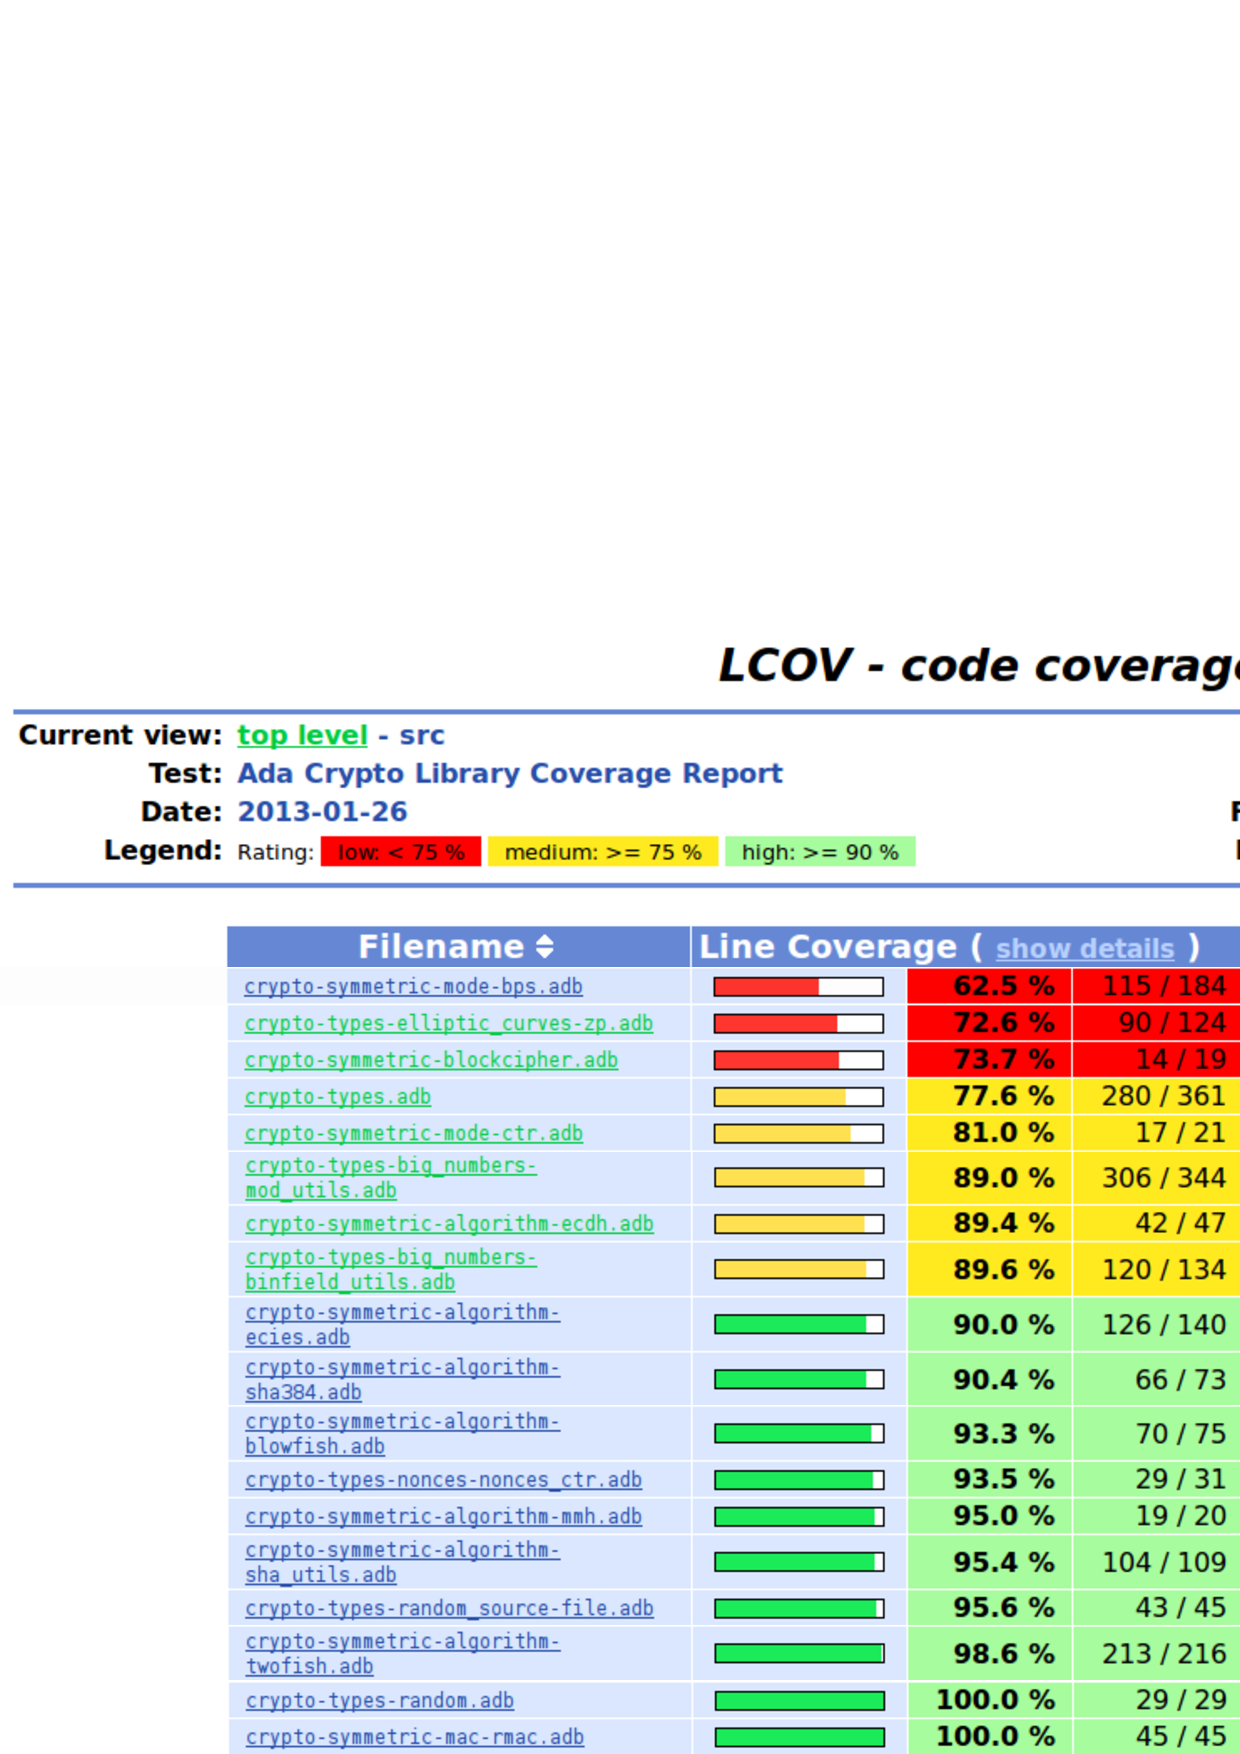
\includegraphics[scale=0.4]{Pictures/LCOV2.pdf} 
  \caption{The current test coverage of the ACL.}\label{LCOVS}
\end{figure}


% Literaturdatenbank
\bibliographystyle{plain} 
\bibliography{crypto}

\end{document}

    
    


